\documentclass[twoside]{book}

% Packages required by doxygen
\usepackage{fixltx2e}
\usepackage{calc}
\usepackage{doxygen}
\usepackage[export]{adjustbox} % also loads graphicx
\usepackage{graphicx}
\usepackage[utf8]{inputenc}
\usepackage{makeidx}
\usepackage{multicol}
\usepackage{multirow}
\PassOptionsToPackage{warn}{textcomp}
\usepackage{textcomp}
\usepackage[nointegrals]{wasysym}
\usepackage[table]{xcolor}

% Font selection
\usepackage[T1]{fontenc}
\usepackage[scaled=.90]{helvet}
\usepackage{courier}
\usepackage{amssymb}
\usepackage{sectsty}
\renewcommand{\familydefault}{\sfdefault}
\allsectionsfont{%
  \fontseries{bc}\selectfont%
  \color{darkgray}%
}
\renewcommand{\DoxyLabelFont}{%
  \fontseries{bc}\selectfont%
  \color{darkgray}%
}
\newcommand{\+}{\discretionary{\mbox{\scriptsize$\hookleftarrow$}}{}{}}

% Page & text layout
\usepackage{geometry}
\geometry{%
  a4paper,%
  top=2.5cm,%
  bottom=2.5cm,%
  left=2.5cm,%
  right=2.5cm%
}
\tolerance=750
\hfuzz=15pt
\hbadness=750
\setlength{\emergencystretch}{15pt}
\setlength{\parindent}{0cm}
\setlength{\parskip}{3ex plus 2ex minus 2ex}
\makeatletter
\renewcommand{\paragraph}{%
  \@startsection{paragraph}{4}{0ex}{-1.0ex}{1.0ex}{%
    \normalfont\normalsize\bfseries\SS@parafont%
  }%
}
\renewcommand{\subparagraph}{%
  \@startsection{subparagraph}{5}{0ex}{-1.0ex}{1.0ex}{%
    \normalfont\normalsize\bfseries\SS@subparafont%
  }%
}
\makeatother

% Headers & footers
\usepackage{fancyhdr}
\pagestyle{fancyplain}
\fancyhead[LE]{\fancyplain{}{\bfseries\thepage}}
\fancyhead[CE]{\fancyplain{}{}}
\fancyhead[RE]{\fancyplain{}{\bfseries\leftmark}}
\fancyhead[LO]{\fancyplain{}{\bfseries\rightmark}}
\fancyhead[CO]{\fancyplain{}{}}
\fancyhead[RO]{\fancyplain{}{\bfseries\thepage}}
\fancyfoot[LE]{\fancyplain{}{}}
\fancyfoot[CE]{\fancyplain{}{}}
\fancyfoot[RE]{\fancyplain{}{\bfseries\scriptsize Generated by Doxygen }}
\fancyfoot[LO]{\fancyplain{}{\bfseries\scriptsize Generated by Doxygen }}
\fancyfoot[CO]{\fancyplain{}{}}
\fancyfoot[RO]{\fancyplain{}{}}
\renewcommand{\footrulewidth}{0.4pt}
\renewcommand{\chaptermark}[1]{%
  \markboth{#1}{}%
}
\renewcommand{\sectionmark}[1]{%
  \markright{\thesection\ #1}%
}

% Indices & bibliography
\usepackage{natbib}
\usepackage[titles]{tocloft}
\setcounter{tocdepth}{3}
\setcounter{secnumdepth}{5}
\makeindex

% Hyperlinks (required, but should be loaded last)
\usepackage{ifpdf}
\ifpdf
  \usepackage[pdftex,pagebackref=true]{hyperref}
\else
  \usepackage[ps2pdf,pagebackref=true]{hyperref}
\fi
\hypersetup{%
  colorlinks=true,%
  linkcolor=blue,%
  citecolor=blue,%
  unicode%
}

% Custom commands
\newcommand{\clearemptydoublepage}{%
  \newpage{\pagestyle{empty}\cleardoublepage}%
}

\usepackage{caption}
\captionsetup{labelsep=space,justification=centering,font={bf},singlelinecheck=off,skip=4pt,position=top}

%===== C O N T E N T S =====

\begin{document}

% Titlepage & ToC
\hypersetup{pageanchor=false,
             bookmarksnumbered=true,
             pdfencoding=unicode
            }
\pagenumbering{alph}
\begin{titlepage}
\vspace*{7cm}
\begin{center}%
{\Large M\+\_\+msg }\\
\vspace*{1cm}
{\large Generated by Doxygen 1.8.14}\\
\end{center}
\end{titlepage}
\clearemptydoublepage
\pagenumbering{roman}
\tableofcontents
\clearemptydoublepage
\pagenumbering{arabic}
\hypersetup{pageanchor=true}

%--- Begin generated contents ---
\chapter{M\+\_\+msg Fortran Library}
\label{index}\hypertarget{index}{}\hypertarget{index_Introduction}{}\section{Introduction}\label{index_Introduction}
logging, journaling, and debugging

 
\chapter{Modules Index}
\section{Modules List}
Here is a list of all modules with brief descriptions\+:\begin{DoxyCompactList}
\item\contentsline{section}{\mbox{\hyperlink{namespacem__journal}{m\+\_\+journal}} \\*\subsubsection*{N\+A\+ME}

M\+\_\+journal(3fm) -\/ \mbox{[}M\+\_\+journal\mbox{]} write program messages to stdout and/or a log file (L\+I\+C\+E\+N\+SE\+:PD) \subsubsection*{S\+Y\+N\+O\+P\+S\+IS}}{\pageref{namespacem__journal}}{}
\item\contentsline{section}{\mbox{\hyperlink{namespacem__msg}{m\+\_\+msg}} }{\pageref{namespacem__msg}}{}
\item\contentsline{section}{\mbox{\hyperlink{namespacem__time}{m\+\_\+time}} }{\pageref{namespacem__time}}{}
\item\contentsline{section}{\mbox{\hyperlink{namespacem__verify}{m\+\_\+verify}} \\*\subsubsection*{N\+A\+ME}

M\+\_\+verify(3fm) -\/ \mbox{[}M\+\_\+verify\mbox{]} a collection of Fortran routines for supporting code development by providing error processing, debugging procedures and unit testing. (L\+I\+C\+E\+N\+SE\+:PD) \subsubsection*{S\+Y\+N\+O\+P\+S\+IS}}{\pageref{namespacem__verify}}{}
\end{DoxyCompactList}

\chapter{Data Type Index}
\section{Data Types List}
Here are the data types with brief descriptions\+:\begin{DoxyCompactList}
\item\contentsline{section}{\mbox{\hyperlink{interfacem__journal_1_1journal}{m\+\_\+journal\+::journal}} \\*\subsubsection*{N\+A\+ME}

journal(3f) -\/ \mbox{[}M\+\_\+journal\mbox{]} provides public message routine, no paging or graphic mode change (L\+I\+C\+E\+N\+SE\+:PD) \subsubsection*{S\+Y\+N\+O\+P\+S\+IS}}{\pageref{interfacem__journal_1_1journal}}{}
\item\contentsline{section}{\mbox{\hyperlink{interfacem__msg_1_1str}{m\+\_\+msg\+::str}} }{\pageref{interfacem__msg_1_1str}}{}
\end{DoxyCompactList}

\chapter{File Index}
\section{File List}
Here is a list of all files with brief descriptions\+:\begin{DoxyCompactList}
\item\contentsline{section}{/home/urbanjs/venus/\+V600/github/\+M\+\_\+msg/src/\mbox{\hyperlink{M__journal_8f90}{M\+\_\+journal.\+f90}} }{\pageref{M__journal_8f90}}{}
\item\contentsline{section}{/home/urbanjs/venus/\+V600/github/\+M\+\_\+msg/src/\mbox{\hyperlink{M__msg_8f90}{M\+\_\+msg.\+f90}} }{\pageref{M__msg_8f90}}{}
\item\contentsline{section}{/home/urbanjs/venus/\+V600/github/\+M\+\_\+msg/src/\mbox{\hyperlink{M__verify_8f90}{M\+\_\+verify.\+f90}} }{\pageref{M__verify_8f90}}{}
\end{DoxyCompactList}

\chapter{Module Documentation}
\hypertarget{namespacem__journal}{}\section{m\+\_\+journal Module Reference}
\label{namespacem__journal}\index{m\+\_\+journal@{m\+\_\+journal}}


\subsubsection*{N\+A\+ME}

M\+\_\+journal(3fm) -\/ \mbox{[}M\+\_\+journal\mbox{]} write program messages to stdout and/or a log file (L\+I\+C\+E\+N\+SE\+:PD) \subsubsection*{S\+Y\+N\+O\+P\+S\+IS} 


\subsection*{Data Types}
\begin{DoxyCompactItemize}
\item 
interface \mbox{\hyperlink{interfacem__journal_1_1journal}{journal}}
\begin{DoxyCompactList}\small\item\em \subsubsection*{N\+A\+ME}

journal(3f) -\/ \mbox{[}M\+\_\+journal\mbox{]} provides public message routine, no paging or graphic mode change (L\+I\+C\+E\+N\+SE\+:PD) \subsubsection*{S\+Y\+N\+O\+P\+S\+IS}\end{DoxyCompactList}\end{DoxyCompactItemize}
\subsection*{Functions/\+Subroutines}
\begin{DoxyCompactItemize}
\item 
subroutine \mbox{\hyperlink{namespacem__journal_a21238c3fc7731703c75eb39233ab529e}{where\+\_\+write\+\_\+message}} (where, msg)
\item 
subroutine \mbox{\hyperlink{namespacem__journal_a24b891eded8ca585a6a72ab0eef7016c}{flush\+\_\+trail}} ()
\item 
subroutine \mbox{\hyperlink{namespacem__journal_a8388800481a5e7ca022b52cfc56b9daf}{set\+\_\+stdout\+\_\+lun}} (iounit)
\item 
subroutine \mbox{\hyperlink{namespacem__journal_a25d0f5da7f7e84e22ab0a583447412b1}{where\+\_\+write\+\_\+message\+\_\+all}} (where, g0, g1, g2, g3, g4, g5, g6, g7, g8, g9, nospace)
\begin{DoxyCompactList}\small\item\em \subsubsection*{N\+A\+ME}

where\+\_\+write\+\_\+message\+\_\+all(3f) -\/ \mbox{[}M\+\_\+journal\mbox{]} converts any standard scalar type to a string and calls journal(3f) (L\+I\+C\+E\+N\+SE\+:PD) \subsubsection*{S\+Y\+N\+O\+P\+S\+IS}\end{DoxyCompactList}\item 
subroutine \mbox{\hyperlink{namespacem__journal_aa86511a7c388f9286c282f6fa933ab58}{write\+\_\+message\+\_\+only}} (message)
\item 
character(len=\+:) function, allocatable \mbox{\hyperlink{namespacem__journal_a9c8074667748f2685122f2b3147e61d5}{now\+\_\+ex}} (format)
\end{DoxyCompactItemize}
\subsection*{Variables}
\begin{DoxyCompactItemize}
\item 
integer, save, private \mbox{\hyperlink{namespacem__journal_a664cf3fd85385b776d30ea589606ad1c}{stdout}} =O\+U\+T\+P\+U\+T\+\_\+\+U\+N\+IT
\item 
logical, save \mbox{\hyperlink{namespacem__journal_a6184fbcebdfa06f0a45ce4c699189b53}{debug}} =.false.
\item 
integer, save \mbox{\hyperlink{namespacem__journal_a47e8e34dc4072b04101027394d688519}{last\+\_\+int}} =0
\end{DoxyCompactItemize}


\subsection{Detailed Description}
\subsubsection*{N\+A\+ME}

M\+\_\+journal(3fm) -\/ \mbox{[}M\+\_\+journal\mbox{]} write program messages to stdout and/or a log file (L\+I\+C\+E\+N\+SE\+:PD) \subsubsection*{S\+Y\+N\+O\+P\+S\+IS}

use, M\+\_\+journal , only \+: journal \subsubsection*{D\+E\+S\+C\+R\+I\+P\+T\+I\+ON}

\begin{DoxyVerb}For interactive programs in particular it is useful if all messages
go thru the JOURNAL(3f) routine. This makes it easy to write messages
to a log file as well as standard output; to toggle time prefixes
on and off; to turn on and off debug-mode messages; control output
paging and create replayable input journals.

The primary use of JOURNAL(3f) is to create journal files for
interactive programs that can be replayed and/or be used to verify
program executions. Typically, you would echo what the user typed to
the trail file as-is, and write output you write to stdout as comments
to the trail file so that the trail file can easily be read back in
(by ignoring comments). So usually things that are read from user
input are using output with WHERE='T' and output that usually goes
to stdout is written with WHERE='SC' in the JOURNAL(3f) call.

 >      :
 >      :
 > character(len=256) userline, output
 > call journal('O','my_trail_file')  ! open trail file
 >      :
 >      :
 > do
 >    read(*,'(a)',iostat=ios) userline  ! read user input
 >    if(ios.ne.0)exit
 >    ! echo user input to trail file
 >    call journal('T',userline)
 >    ! assume user input causes values i1, i2, and i3 to be calculated
 >    write(output,'(i0,1x,i0,1x)')i1,i2,i3 ! build an output line
 >    ! write output to stdout and as comment to trail file
 >    call journal(output)
 >    !or you can specify the WHERE parameter and up to ten scalar values
 >    call journal('SC','i1=',i1,'i2=',i2,'i3=',i3)
 > enddo

In this example an output line was built with an internal write; but calls
to journal(3f) with numeric values with and without advancing I/O turned on
are often used for simpler output:

   I=10
   R=20.3
   ! write to stdout and trail file without advancing I/O
   call journal('+SC','I=',i)
   call journal('SC','AND R=',r)

writes to the trail file are ignored unless a trail file was opened with

   CALL JOURNAL('O',filename)


So that routines that do their output via JOURNAL(3f) can be used with and
without programs generating trail files. That is, destinations 'T' and 'C'
are ignored unless a trail file has been requested.

With no parameters, the trail file is flushed.
\end{DoxyVerb}


\subsubsection*{E\+X\+A\+M\+P\+L\+ES}

\begin{DoxyVerb}The man(1) page for journal(3f) describes all the options for the WHERE field.
In addition to being used to generate a journal, the routine can be used for
producing optional debug messages and timing information.

Sample program for debug messages:

  program demo_journal
  !! showing creating debug messages
  use M_journal, only : journal
  implicit none
  !! produces no output because trail is not on
  call journal('D','*demo* DEBUG MESSAGE 001 IGNORED')
  !! turn on debug messages
  call journal('>','debug on')
  !! produces output on stdout because debug mode
  !! is on but no named trail file
  call journal('D','*demo* DEBUG MESSAGE 002 ON STDOUT')
  !! open trail file
  call journal('O','mytrail.txt')
  !! debug messages now go to the trail file
  call journal('D','*demo* DEBUG MESSAGE 003 TO TRAIL')
  !! close trail file so messages go to stdout again
  call journal('O','')
  !! debug on stdout now
  call journal('D','*demo* DEBUG MESSAGE 004 TO STDOUT')
  call journal('<','debug off')
  !! back to no output from the next message
  call journal('D','*demo* DEBUG MESSAGE 005 IGNORED')
  end program demo_journal
\end{DoxyVerb}


Sample program for trail messages with optional timing information\+:

program testit use M\+\_\+journal,only \+: journal implicit none call journal(\textquotesingle{}a single string A -\/should be on S\textquotesingle{})

! add time prefix to output call journal(\textquotesingle{}\textquotesingle{},\textquotesingle{}Y-\/M-\/DTh\+:m\+:s.xu\+:b\textquotesingle{}) call journal(\textquotesingle{}a single string B -\/should be on S with prefix\textquotesingle{}) call journal(\textquotesingle{}\textquotesingle{},\textquotesingle{}C\+P\+U\+\_\+\+T\+I\+ME\+: c\+:C\+A\+L\+LS\+: C\+: b\textquotesingle{}) ! change time prefix call journal(\textquotesingle{}a single string B-\/1 -\/should be on S with prefix\textquotesingle{}) call journal(\textquotesingle{}a single string B-\/2 -\/should be on S with prefix\textquotesingle{}) call journal(\textquotesingle{}a single string B-\/3 -\/should be on S with prefix\textquotesingle{}) ! Other useful time formats\+: ! E -- Unix Epoch time ! e -- integer value of Unix Epoch time ! C -- number of times this format is used ! c -- C\+P\+U\+\_\+time(3f) output ! S -- seconds since last use of this format ! k -- C\+PU time in seconds from system\+\_\+clock call journal(\textquotesingle{}\textquotesingle{},\textquotesingle{}\textquotesingle{}) ! turn off time prefix ! call journal(\textquotesingle{}a single string C -\/should be on S\textquotesingle{}) ! call journal(\textquotesingle{}O\textquotesingle{},\textquotesingle{}aaa.\+out\textquotesingle{}) ! turn on trail file call journal(\textquotesingle{}a single string D -\/should be on SC\textquotesingle{}) call journal(\textquotesingle{}a single string E -\/should be on SC\textquotesingle{}) call journal(\textquotesingle{}a single string F -\/should be on SC\textquotesingle{}) call journal(\textquotesingle{}O\textquotesingle{},\textquotesingle{}\textquotesingle{}) ! turn off trail file ! call journal(\textquotesingle{}a single string G -\/should be on S\textquotesingle{}) call journal(\textquotesingle{}a single string H -\/should be on S\textquotesingle{}) call journal(\textquotesingle{}a single string I -\/should be on S\textquotesingle{})

! build one line of output with intrinsic scalar values added call journal(\textquotesingle{}+sc\textquotesingle{},\textquotesingle{}A\+P\+P\+E\+ND\+:\textquotesingle{}) call journal(\textquotesingle{}+sc\textquotesingle{},\textquotesingle{} integer\textquotesingle{}, 1234) call journal(\textquotesingle{}+sc\textquotesingle{},\textquotesingle{} and real\textquotesingle{}, 1234.\+5678) call journal(\textquotesingle{}+sc\textquotesingle{},\textquotesingle{} and double\textquotesingle{},1234567890.\+123456d0) call journal(\textquotesingle{}+sc\textquotesingle{},\textquotesingle{} and logical\textquotesingle{}, .true.) call journal(\textquotesingle{}sc\textquotesingle{},\textquotesingle{}\textquotesingle{}) ! end program testit

\subsubsection*{A\+U\+T\+H\+OR}

John S. Urban \subsubsection*{L\+I\+C\+E\+N\+SE}

Public Domain 

\subsection{Function/\+Subroutine Documentation}
\mbox{\Hypertarget{namespacem__journal_a24b891eded8ca585a6a72ab0eef7016c}\label{namespacem__journal_a24b891eded8ca585a6a72ab0eef7016c}} 
\index{m\+\_\+journal@{m\+\_\+journal}!flush\+\_\+trail@{flush\+\_\+trail}}
\index{flush\+\_\+trail@{flush\+\_\+trail}!m\+\_\+journal@{m\+\_\+journal}}
\subsubsection{\texorpdfstring{flush\+\_\+trail()}{flush\_trail()}}
{\footnotesize\ttfamily subroutine m\+\_\+journal\+::flush\+\_\+trail (\begin{DoxyParamCaption}{ }\end{DoxyParamCaption})\hspace{0.3cm}{\ttfamily [private]}}



References where\+\_\+write\+\_\+message().

Here is the call graph for this function\+:\nopagebreak
\begin{figure}[H]
\begin{center}
\leavevmode
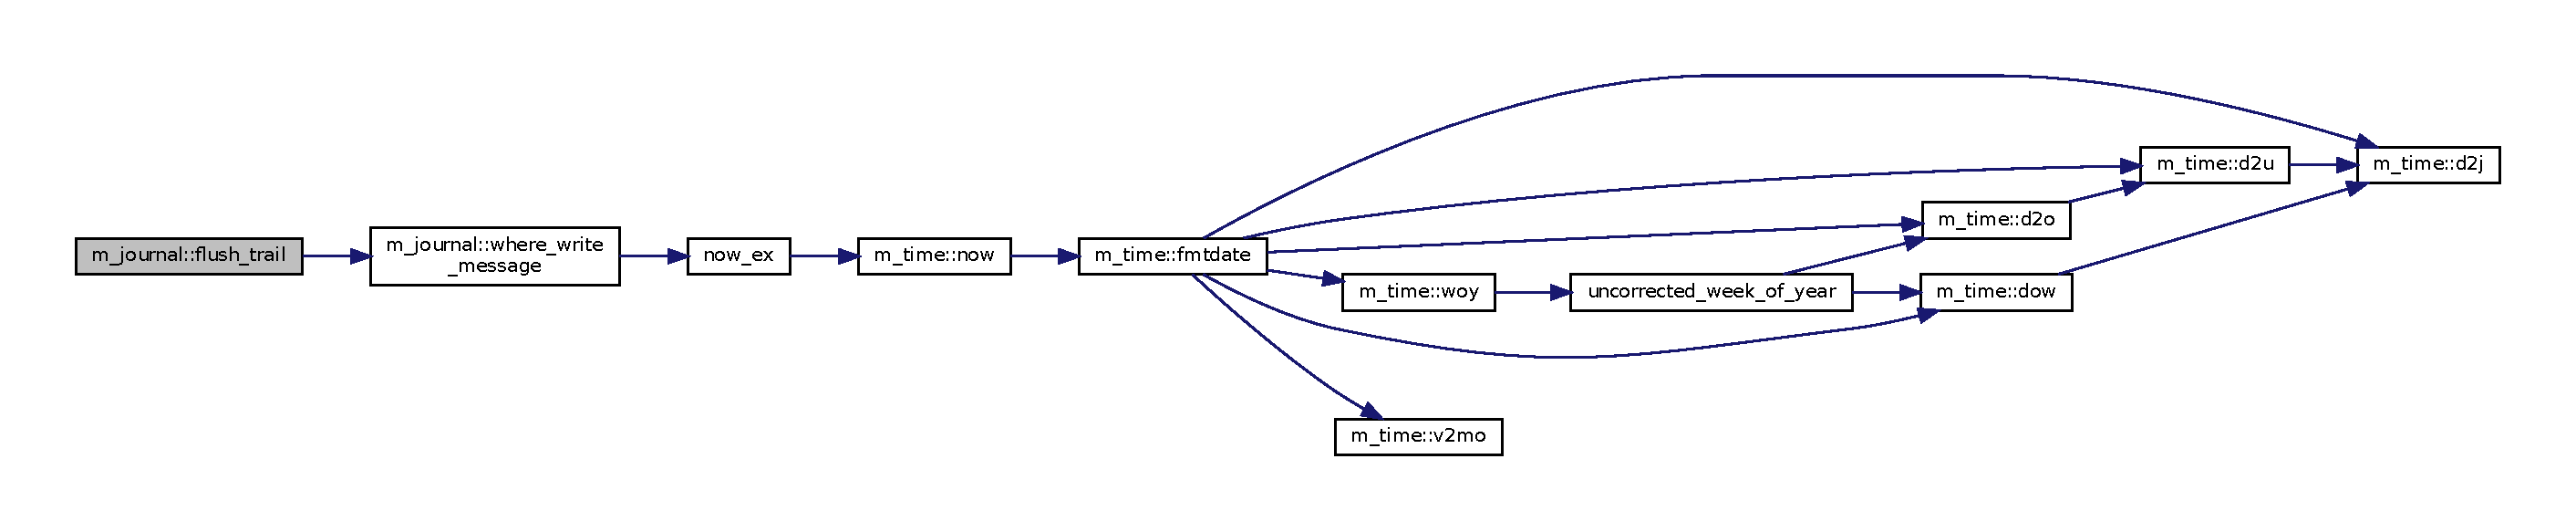
\includegraphics[width=350pt]{namespacem__journal_a24b891eded8ca585a6a72ab0eef7016c_cgraph}
\end{center}
\end{figure}
\mbox{\Hypertarget{namespacem__journal_a9c8074667748f2685122f2b3147e61d5}\label{namespacem__journal_a9c8074667748f2685122f2b3147e61d5}} 
\index{m\+\_\+journal@{m\+\_\+journal}!now\+\_\+ex@{now\+\_\+ex}}
\index{now\+\_\+ex@{now\+\_\+ex}!m\+\_\+journal@{m\+\_\+journal}}
\subsubsection{\texorpdfstring{now\+\_\+ex()}{now\_ex()}}
{\footnotesize\ttfamily character(len=\+:) function, allocatable m\+\_\+journal\+::now\+\_\+ex (\begin{DoxyParamCaption}\item[{character(len=$\ast$), intent(in), optional}]{format }\end{DoxyParamCaption})\hspace{0.3cm}{\ttfamily [private]}}



References m\+\_\+time\+::now(), and now\+\_\+ex().

Here is the call graph for this function\+:\nopagebreak
\begin{figure}[H]
\begin{center}
\leavevmode
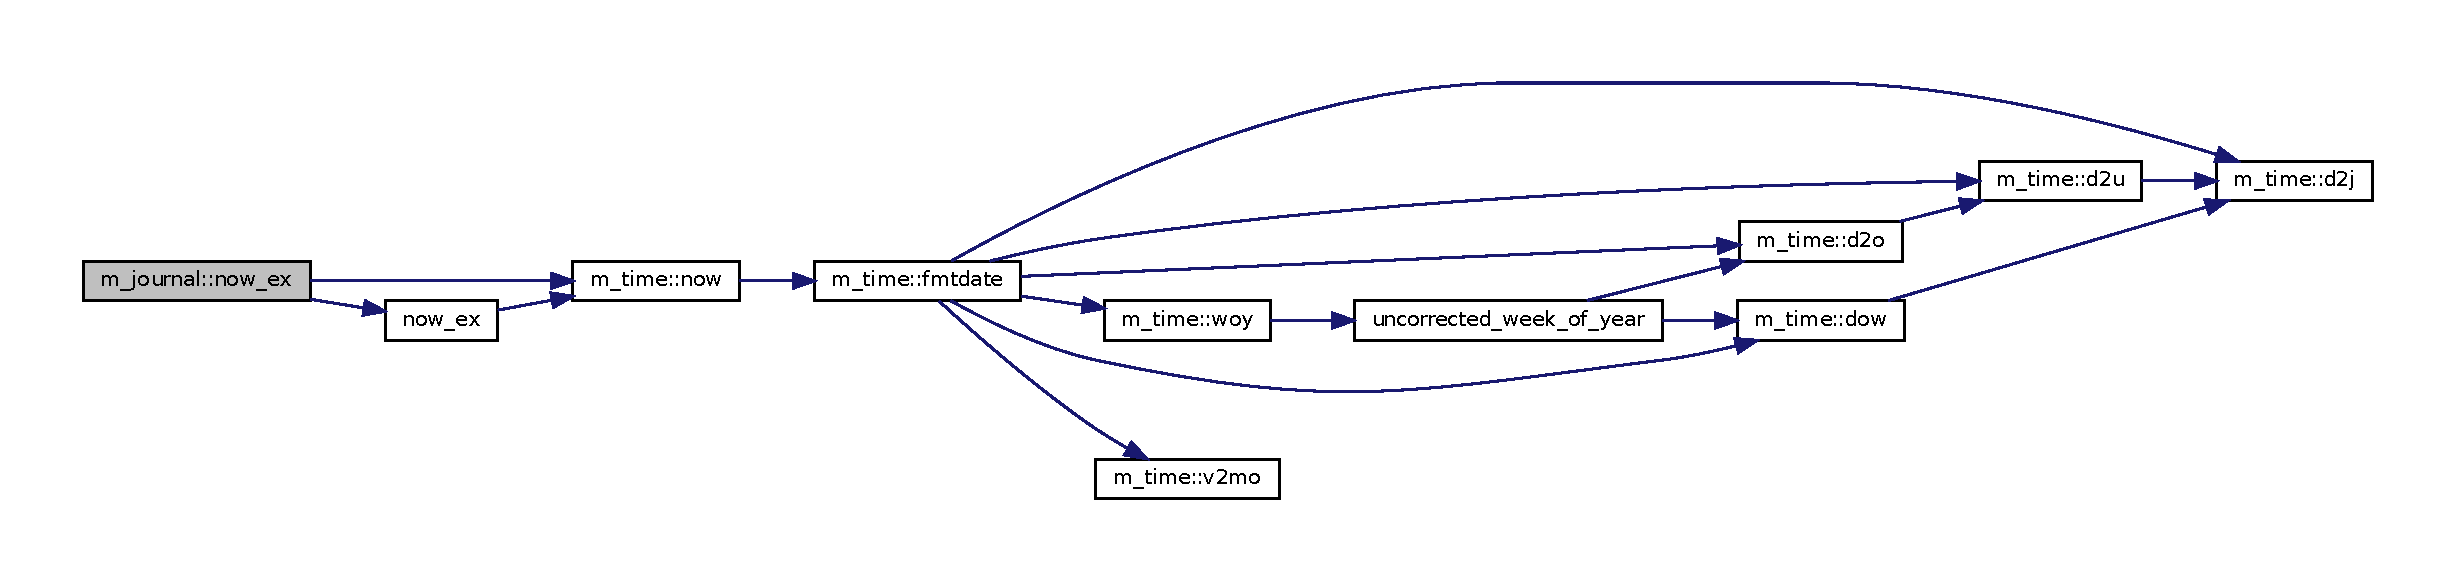
\includegraphics[width=350pt]{namespacem__journal_a9c8074667748f2685122f2b3147e61d5_cgraph}
\end{center}
\end{figure}
\mbox{\Hypertarget{namespacem__journal_a8388800481a5e7ca022b52cfc56b9daf}\label{namespacem__journal_a8388800481a5e7ca022b52cfc56b9daf}} 
\index{m\+\_\+journal@{m\+\_\+journal}!set\+\_\+stdout\+\_\+lun@{set\+\_\+stdout\+\_\+lun}}
\index{set\+\_\+stdout\+\_\+lun@{set\+\_\+stdout\+\_\+lun}!m\+\_\+journal@{m\+\_\+journal}}
\subsubsection{\texorpdfstring{set\+\_\+stdout\+\_\+lun()}{set\_stdout\_lun()}}
{\footnotesize\ttfamily subroutine m\+\_\+journal\+::set\+\_\+stdout\+\_\+lun (\begin{DoxyParamCaption}\item[{integer, intent(in)}]{iounit }\end{DoxyParamCaption})\hspace{0.3cm}{\ttfamily [private]}}



References stdout.

\mbox{\Hypertarget{namespacem__journal_a21238c3fc7731703c75eb39233ab529e}\label{namespacem__journal_a21238c3fc7731703c75eb39233ab529e}} 
\index{m\+\_\+journal@{m\+\_\+journal}!where\+\_\+write\+\_\+message@{where\+\_\+write\+\_\+message}}
\index{where\+\_\+write\+\_\+message@{where\+\_\+write\+\_\+message}!m\+\_\+journal@{m\+\_\+journal}}
\subsubsection{\texorpdfstring{where\+\_\+write\+\_\+message()}{where\_write\_message()}}
{\footnotesize\ttfamily subroutine m\+\_\+journal\+::where\+\_\+write\+\_\+message (\begin{DoxyParamCaption}\item[{character(len=$\ast$), intent(in)}]{where,  }\item[{character(len=$\ast$), intent(in)}]{msg }\end{DoxyParamCaption})\hspace{0.3cm}{\ttfamily [private]}}



References debug, last\+\_\+int, now\+\_\+ex(), and stdout.

Here is the call graph for this function\+:\nopagebreak
\begin{figure}[H]
\begin{center}
\leavevmode
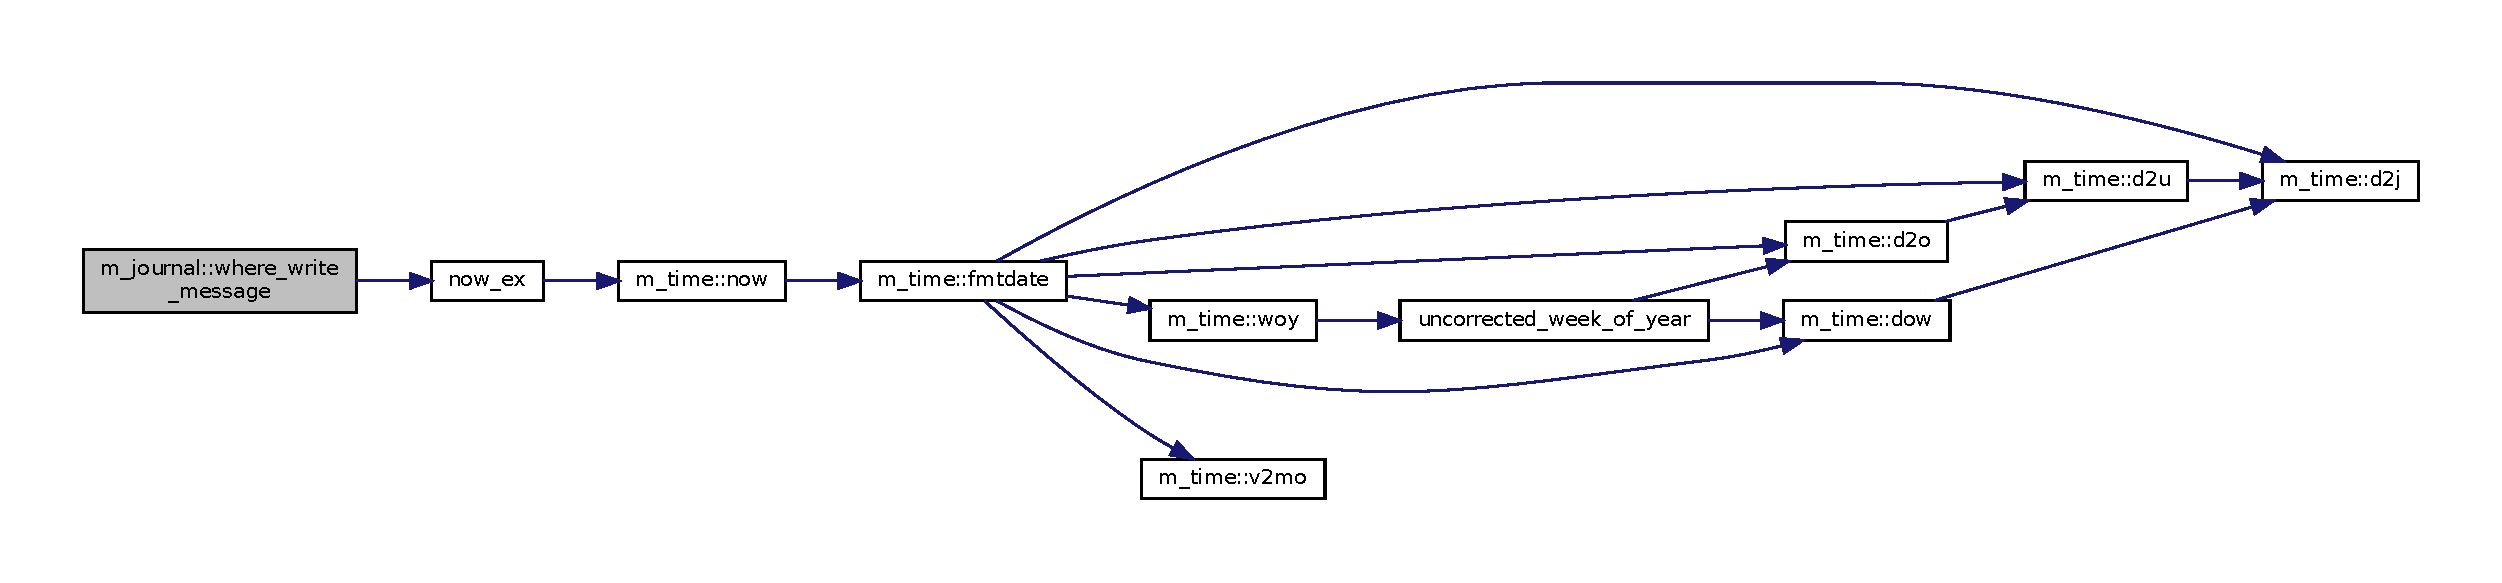
\includegraphics[width=350pt]{namespacem__journal_a21238c3fc7731703c75eb39233ab529e_cgraph}
\end{center}
\end{figure}
Here is the caller graph for this function\+:\nopagebreak
\begin{figure}[H]
\begin{center}
\leavevmode
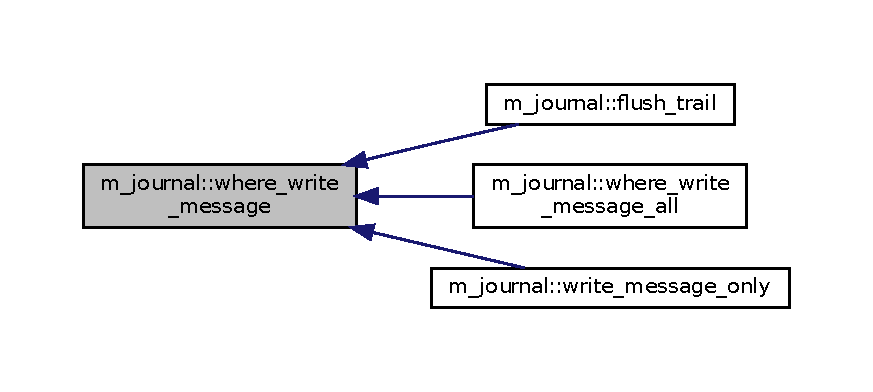
\includegraphics[width=350pt]{namespacem__journal_a21238c3fc7731703c75eb39233ab529e_icgraph}
\end{center}
\end{figure}
\mbox{\Hypertarget{namespacem__journal_a25d0f5da7f7e84e22ab0a583447412b1}\label{namespacem__journal_a25d0f5da7f7e84e22ab0a583447412b1}} 
\index{m\+\_\+journal@{m\+\_\+journal}!where\+\_\+write\+\_\+message\+\_\+all@{where\+\_\+write\+\_\+message\+\_\+all}}
\index{where\+\_\+write\+\_\+message\+\_\+all@{where\+\_\+write\+\_\+message\+\_\+all}!m\+\_\+journal@{m\+\_\+journal}}
\subsubsection{\texorpdfstring{where\+\_\+write\+\_\+message\+\_\+all()}{where\_write\_message\_all()}}
{\footnotesize\ttfamily subroutine m\+\_\+journal\+::where\+\_\+write\+\_\+message\+\_\+all (\begin{DoxyParamCaption}\item[{character(len=$\ast$), intent(in)}]{where,  }\item[{class($\ast$), intent(in)}]{g0,  }\item[{class($\ast$), intent(in), optional}]{g1,  }\item[{class($\ast$), intent(in), optional}]{g2,  }\item[{class($\ast$), intent(in), optional}]{g3,  }\item[{class($\ast$), intent(in), optional}]{g4,  }\item[{class($\ast$), intent(in), optional}]{g5,  }\item[{class($\ast$), intent(in), optional}]{g6,  }\item[{class($\ast$), intent(in), optional}]{g7,  }\item[{class($\ast$), intent(in), optional}]{g8,  }\item[{class($\ast$), intent(in), optional}]{g9,  }\item[{logical, intent(in), optional}]{nospace }\end{DoxyParamCaption})\hspace{0.3cm}{\ttfamily [private]}}



\subsubsection*{N\+A\+ME}

where\+\_\+write\+\_\+message\+\_\+all(3f) -\/ \mbox{[}M\+\_\+journal\mbox{]} converts any standard scalar type to a string and calls journal(3f) (L\+I\+C\+E\+N\+SE\+:PD) \subsubsection*{S\+Y\+N\+O\+P\+S\+IS}

subroutine where\+\_\+write\+\_\+message\+\_\+all(where,g0,g1,g2g3,g4,g5,g6,g7,g8,g9,nospace)

character(len=$\ast$),intent(in) \+:\+: where class($\ast$),intent(in) \+:\+: g0 class($\ast$),intent(in),optional \+:\+: g1,g2,g3,g4,g5,g6,g7,g8,g9 logical,intent(in),optional \+:\+: nospace

\subsubsection*{D\+E\+S\+C\+R\+I\+P\+T\+I\+ON}

where\+\_\+write\+\_\+message\+\_\+all(3f) builds and writes a space-\/separated string from up to nine scalar values.

\subsubsection*{O\+P\+T\+I\+O\+NS}

\begin{DoxyVerb}where    string designating where to write message, as with journal(3f)
g0       value to print. May
         be of type INTEGER, LOGICAL, REAL, DOUBLEPRECISION, COMPLEX,
         or CHARACTER.
g[1-9]   optional additional values to print the value of after g0.
nospace  if nospace=.true., then no spaces are added between values
\end{DoxyVerb}
 \subsubsection*{R\+E\+T\+U\+R\+NS}

where\+\_\+write\+\_\+message\+\_\+all description to print

\subsubsection*{E\+X\+A\+M\+P\+L\+ES}

Sample program\+:

program demo\+\_\+wm\+\_\+all use M\+\_\+journal, only \+: where\+\_\+write\+\_\+message\+\_\+all implicit none end program program demo\+\_\+wm\+\_\+all \subsubsection*{A\+U\+T\+H\+OR}

John S. Urban \subsubsection*{L\+I\+C\+E\+N\+SE}

Public Domain 

References where\+\_\+write\+\_\+message().

Here is the call graph for this function\+:\nopagebreak
\begin{figure}[H]
\begin{center}
\leavevmode
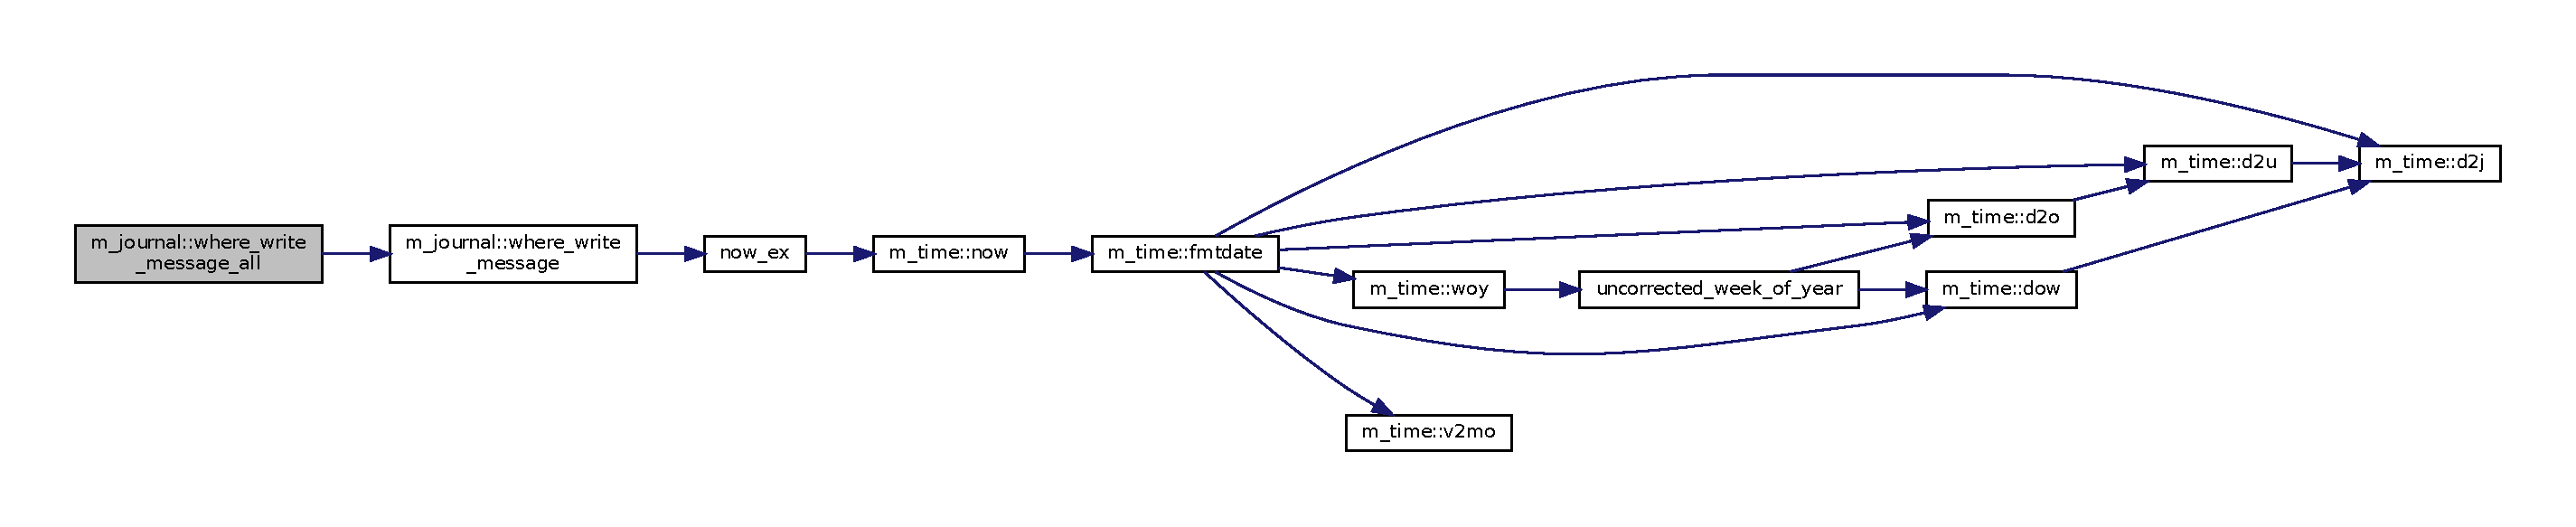
\includegraphics[width=350pt]{namespacem__journal_a25d0f5da7f7e84e22ab0a583447412b1_cgraph}
\end{center}
\end{figure}
\mbox{\Hypertarget{namespacem__journal_aa86511a7c388f9286c282f6fa933ab58}\label{namespacem__journal_aa86511a7c388f9286c282f6fa933ab58}} 
\index{m\+\_\+journal@{m\+\_\+journal}!write\+\_\+message\+\_\+only@{write\+\_\+message\+\_\+only}}
\index{write\+\_\+message\+\_\+only@{write\+\_\+message\+\_\+only}!m\+\_\+journal@{m\+\_\+journal}}
\subsubsection{\texorpdfstring{write\+\_\+message\+\_\+only()}{write\_message\_only()}}
{\footnotesize\ttfamily subroutine m\+\_\+journal\+::write\+\_\+message\+\_\+only (\begin{DoxyParamCaption}\item[{character(len=$\ast$), intent(in)}]{message }\end{DoxyParamCaption})\hspace{0.3cm}{\ttfamily [private]}}



References where\+\_\+write\+\_\+message().

Here is the call graph for this function\+:\nopagebreak
\begin{figure}[H]
\begin{center}
\leavevmode
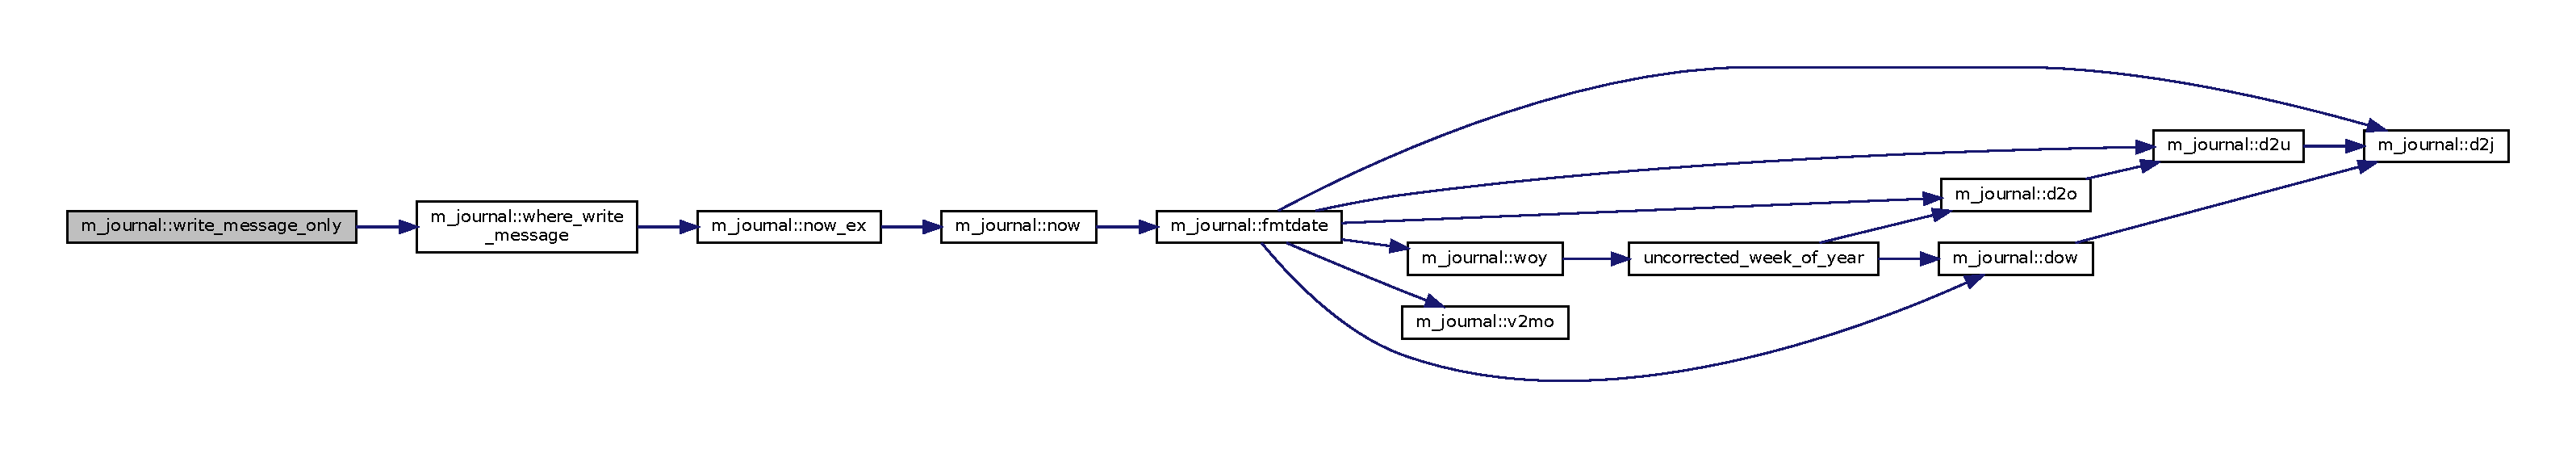
\includegraphics[width=350pt]{namespacem__journal_aa86511a7c388f9286c282f6fa933ab58_cgraph}
\end{center}
\end{figure}


\subsection{Variable Documentation}
\mbox{\Hypertarget{namespacem__journal_a6184fbcebdfa06f0a45ce4c699189b53}\label{namespacem__journal_a6184fbcebdfa06f0a45ce4c699189b53}} 
\index{m\+\_\+journal@{m\+\_\+journal}!debug@{debug}}
\index{debug@{debug}!m\+\_\+journal@{m\+\_\+journal}}
\subsubsection{\texorpdfstring{debug}{debug}}
{\footnotesize\ttfamily logical, save m\+\_\+journal\+::debug =.false.\hspace{0.3cm}{\ttfamily [private]}}

\mbox{\Hypertarget{namespacem__journal_a47e8e34dc4072b04101027394d688519}\label{namespacem__journal_a47e8e34dc4072b04101027394d688519}} 
\index{m\+\_\+journal@{m\+\_\+journal}!last\+\_\+int@{last\+\_\+int}}
\index{last\+\_\+int@{last\+\_\+int}!m\+\_\+journal@{m\+\_\+journal}}
\subsubsection{\texorpdfstring{last\+\_\+int}{last\_int}}
{\footnotesize\ttfamily integer, save m\+\_\+journal\+::last\+\_\+int =0\hspace{0.3cm}{\ttfamily [private]}}

\mbox{\Hypertarget{namespacem__journal_a664cf3fd85385b776d30ea589606ad1c}\label{namespacem__journal_a664cf3fd85385b776d30ea589606ad1c}} 
\index{m\+\_\+journal@{m\+\_\+journal}!stdout@{stdout}}
\index{stdout@{stdout}!m\+\_\+journal@{m\+\_\+journal}}
\subsubsection{\texorpdfstring{stdout}{stdout}}
{\footnotesize\ttfamily integer, save, private m\+\_\+journal\+::stdout =O\+U\+T\+P\+U\+T\+\_\+\+U\+N\+IT\hspace{0.3cm}{\ttfamily [private]}}


\hypertarget{namespacem__msg}{}\section{m\+\_\+msg Module Reference}
\label{namespacem__msg}\index{m\+\_\+msg@{m\+\_\+msg}}
\subsection*{Data Types}
\begin{DoxyCompactItemize}
\item 
interface \mbox{\hyperlink{interfacem__msg_1_1str}{str}}
\end{DoxyCompactItemize}
\subsection*{Functions/\+Subroutines}
\begin{DoxyCompactItemize}
\item 
character(len=\+:) function, allocatable \mbox{\hyperlink{namespacem__msg_a2e19921e3e57824c605acd4f7c83ad83}{msg\+\_\+scalar}} (generic0, generic1, generic2, generic3, generic4, generic5, generic6, generic7, generic8, generic9, generica, genericb, genericc, genericd, generice, genericf, genericg, generich, generici, genericj, nospace)
\begin{DoxyCompactList}\small\item\em \subsubsection*{N\+A\+ME}

str(3f) -\/ \mbox{[}M\+\_\+msg\mbox{]} converts any standard scalar type to a string (L\+I\+C\+E\+N\+SE\+:PD) \end{DoxyCompactList}\item 
character(len=\+:) function, allocatable \mbox{\hyperlink{namespacem__msg_a069f107ba79e88a43dd5c835080eff1a}{msg\+\_\+one}} (generic0, generic1, generic2, generic3, generic4, generic5, generic6, generic7, generic8, generic9, nospace)
\end{DoxyCompactItemize}


\subsection{Function/\+Subroutine Documentation}
\mbox{\Hypertarget{namespacem__msg_a069f107ba79e88a43dd5c835080eff1a}\label{namespacem__msg_a069f107ba79e88a43dd5c835080eff1a}} 
\index{m\+\_\+msg@{m\+\_\+msg}!msg\+\_\+one@{msg\+\_\+one}}
\index{msg\+\_\+one@{msg\+\_\+one}!m\+\_\+msg@{m\+\_\+msg}}
\subsubsection{\texorpdfstring{msg\+\_\+one()}{msg\_one()}}
{\footnotesize\ttfamily character(len=\+:) function, allocatable m\+\_\+msg\+::msg\+\_\+one (\begin{DoxyParamCaption}\item[{class($\ast$), dimension(\+:), intent(in)}]{generic0,  }\item[{class($\ast$), dimension(\+:), intent(in), optional}]{generic1,  }\item[{class($\ast$), dimension(\+:), intent(in), optional}]{generic2,  }\item[{class($\ast$), dimension(\+:), intent(in), optional}]{generic3,  }\item[{class($\ast$), dimension(\+:), intent(in), optional}]{generic4,  }\item[{class($\ast$), dimension(\+:), intent(in), optional}]{generic5,  }\item[{class($\ast$), dimension(\+:), intent(in), optional}]{generic6,  }\item[{class($\ast$), dimension(\+:), intent(in), optional}]{generic7,  }\item[{class($\ast$), dimension(\+:), intent(in), optional}]{generic8,  }\item[{class($\ast$), dimension(\+:), intent(in), optional}]{generic9,  }\item[{logical, intent(in), optional}]{nospace }\end{DoxyParamCaption})\hspace{0.3cm}{\ttfamily [private]}}



References print\+\_\+generic().

Here is the call graph for this function\+:\nopagebreak
\begin{figure}[H]
\begin{center}
\leavevmode
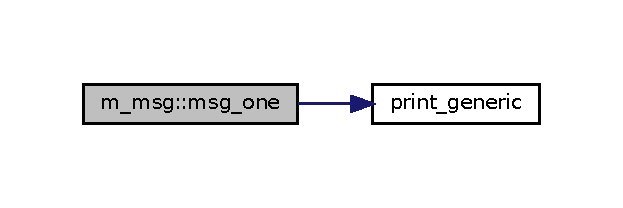
\includegraphics[width=299pt]{namespacem__msg_a069f107ba79e88a43dd5c835080eff1a_cgraph}
\end{center}
\end{figure}
\mbox{\Hypertarget{namespacem__msg_a2e19921e3e57824c605acd4f7c83ad83}\label{namespacem__msg_a2e19921e3e57824c605acd4f7c83ad83}} 
\index{m\+\_\+msg@{m\+\_\+msg}!msg\+\_\+scalar@{msg\+\_\+scalar}}
\index{msg\+\_\+scalar@{msg\+\_\+scalar}!m\+\_\+msg@{m\+\_\+msg}}
\subsubsection{\texorpdfstring{msg\+\_\+scalar()}{msg\_scalar()}}
{\footnotesize\ttfamily character(len=\+:) function, allocatable m\+\_\+msg\+::msg\+\_\+scalar (\begin{DoxyParamCaption}\item[{class($\ast$), intent(in), optional}]{generic0,  }\item[{class($\ast$), intent(in), optional}]{generic1,  }\item[{class($\ast$), intent(in), optional}]{generic2,  }\item[{class($\ast$), intent(in), optional}]{generic3,  }\item[{class($\ast$), intent(in), optional}]{generic4,  }\item[{class($\ast$), intent(in), optional}]{generic5,  }\item[{class($\ast$), intent(in), optional}]{generic6,  }\item[{class($\ast$), intent(in), optional}]{generic7,  }\item[{class($\ast$), intent(in), optional}]{generic8,  }\item[{class($\ast$), intent(in), optional}]{generic9,  }\item[{class($\ast$), intent(in), optional}]{generica,  }\item[{class($\ast$), intent(in), optional}]{genericb,  }\item[{class($\ast$), intent(in), optional}]{genericc,  }\item[{class($\ast$), intent(in), optional}]{genericd,  }\item[{class($\ast$), intent(in), optional}]{generice,  }\item[{class($\ast$), intent(in), optional}]{genericf,  }\item[{class($\ast$), intent(in), optional}]{genericg,  }\item[{class($\ast$), intent(in), optional}]{generich,  }\item[{class($\ast$), intent(in), optional}]{generici,  }\item[{class($\ast$), intent(in), optional}]{genericj,  }\item[{logical, intent(in), optional}]{nospace }\end{DoxyParamCaption})\hspace{0.3cm}{\ttfamily [private]}}



\subsubsection*{N\+A\+ME}

str(3f) -\/ \mbox{[}M\+\_\+msg\mbox{]} converts any standard scalar type to a string (L\+I\+C\+E\+N\+SE\+:PD) 

\subsubsection*{S\+Y\+N\+O\+P\+S\+IS}

\begin{DoxyVerb} function str(g0,g1,g2,g3,g4,g5,g6,g7,g8,g9,&
 & ga,gb,gc,gd,ge,gf,gg,gh,gi,gj,nospace)

  class(*),intent(in),optional  :: g0,g1,g2,g3,g4,g5,g6,g7,g8,g9
  class(*),intent(in),optional  :: ga,gb,gc,gd,ge,gf,gg,gh,gi,gj
  logical,intent(in),optional   :: nospace
  character,len=(:),allocatable :: str
\end{DoxyVerb}


\subsubsection*{D\+E\+S\+C\+R\+I\+P\+T\+I\+ON}

str(3f) builds a space-\/separated string from up to twenty scalar values.

\subsubsection*{O\+P\+T\+I\+O\+NS}

g\mbox{[}0-\/9a-\/j\mbox{]} optional value to print the value of after the message. May be of type I\+N\+T\+E\+G\+ER, L\+O\+G\+I\+C\+AL, R\+E\+AL, D\+O\+U\+B\+L\+E\+P\+R\+E\+C\+I\+S\+I\+ON, C\+O\+M\+P\+L\+EX, or C\+H\+A\+R\+A\+C\+T\+ER.

Optionally, all the generic values can be single-\/dimensioned arrays. Currently, mixing scalar arguments and array arguments is not supported.

nospace if nospace=.true., then no spaces are added between values

\subsubsection*{R\+E\+T\+U\+R\+NS}

str description to print

\subsubsection*{E\+X\+A\+M\+P\+L\+ES}

Sample program\+:

program demo\+\_\+msg use M\+\_\+msg, only \+: str implicit none character(len=\+:),allocatable \+:\+: pr character(len=\+:),allocatable \+:\+: frmt integer \+:\+: biggest

pr=str(\textquotesingle{}H\+U\+G\+E(3f) integers\textquotesingle{},huge(0),\& \&\textquotesingle{}and real\textquotesingle{},huge(0.\+0),\textquotesingle{}and double\textquotesingle{},huge(0.\+0d0)) write($\ast$,\textquotesingle{}(a)\textquotesingle{})pr pr=str(\textquotesingle{}real \+:\textquotesingle{},huge(0.\+0),0.\+0,12345.\+6789,tiny(0.\+0) ) write($\ast$,\textquotesingle{}(a)\textquotesingle{})pr pr=str(\textquotesingle{}doubleprecision \+:\textquotesingle{},huge(0.\+0d0),0.\+0d0,12345.\+6789d0,tiny(0.\+0d0) ) write($\ast$,\textquotesingle{}(a)\textquotesingle{})pr pr=str(\textquotesingle{}complex \+:\textquotesingle{},cmplx(huge(0.\+0),tiny(0.\+0)) ) write($\ast$,\textquotesingle{}(a)\textquotesingle{})pr

! create a format on the fly biggest=huge(0) frmt=str(\textquotesingle{}($\ast$(i\textquotesingle{},int(log10(real(biggest))),\textquotesingle{}\+:,1x))\textquotesingle{},nospace=.true.) write($\ast$,$\ast$)\textquotesingle{}format=\textquotesingle{},frmt

! although it will often work, using str(3f) ! in an I/O statement is not recommended ! because if an error occurs str(3f) will try ! to write while part of an I/O statement ! which not all compilers can handle and is currently non-\/standard write($\ast$,$\ast$)str(\textquotesingle{}program will now stop\textquotesingle{})

end program demo\+\_\+msg

Output

H\+U\+G\+E(3f) integers 2147483647 and real 3.\+40282347E+38 and double 1.\+7976931348623157E+308 real \+: 3.\+40282347E+38 0.\+00000000 12345.\+6787 1.\+17549435E-\/38 doubleprecision \+: 1.\+7976931348623157E+308 0.\+0000000000000000 12345.\+678900000001 2.\+2250738585072014E-\/308 complex \+: (3.\+40282347E+38,1.\+17549435E-\/38) format=($\ast$(i9\+:,1x)) program will now stop

\subsubsection*{A\+U\+T\+H\+OR}

John S. Urban

\subsubsection*{L\+I\+C\+E\+N\+SE}

Public Domain 

References print\+\_\+generic().

Here is the call graph for this function\+:\nopagebreak
\begin{figure}[H]
\begin{center}
\leavevmode
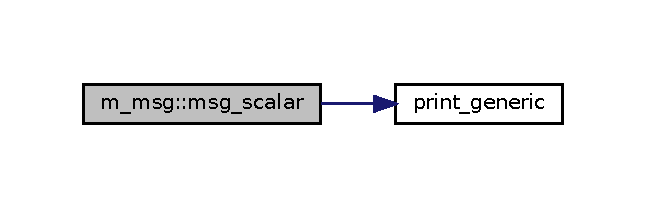
\includegraphics[width=310pt]{namespacem__msg_a2e19921e3e57824c605acd4f7c83ad83_cgraph}
\end{center}
\end{figure}

\hypertarget{namespacem__time}{}\section{m\+\_\+time Module Reference}
\label{namespacem__time}\index{m\+\_\+time@{m\+\_\+time}}
\subsection*{Functions/\+Subroutines}
\begin{DoxyCompactItemize}
\item 
subroutine, public \mbox{\hyperlink{namespacem__time_a12cbfe4ebed008f4cdf88df4358df8ad}{d2j}} (dat, julian, ierr)
\item 
subroutine, public \mbox{\hyperlink{namespacem__time_a4da84079c6587a8aaa8ef32169a84cc5}{j2d}} (dat, julian, ierr)
\item 
subroutine, public \mbox{\hyperlink{namespacem__time_ac4bd98688e1277ab6cfc16697331406c}{d2u}} (dat, unixtime, ierr)
\item 
subroutine, public \mbox{\hyperlink{namespacem__time_a6c01c810eb2acce767d2f24b9aaefa56}{u2d}} (dat, unixtime, ierr)
\item 
integer function, public \mbox{\hyperlink{namespacem__time_a727dd77bbd4a5d0e3947c5d303845947}{d2o}} (dat)
\item 
character(len=\+:) function, allocatable, public \mbox{\hyperlink{namespacem__time_a6f28cf00e4998bb50bb503f5e4bd3f77}{v2mo}} (imonth)
\item 
character(len=\+:) function, allocatable, public \mbox{\hyperlink{namespacem__time_a6b5e87be0e510ff268c1ecfbf67a3bdb}{now}} (format)
\item 
character(len=\+:) function, allocatable, public \mbox{\hyperlink{namespacem__time_a2cb84c9b8af4f395b76aed76e1431328}{fmtdate}} (values, format)
\item 
subroutine, public \mbox{\hyperlink{namespacem__time_a0ec30ca32f18ec409bbbef046a9e73f0}{fmtdate\+\_\+usage}} (ii)
\item 
subroutine, public \mbox{\hyperlink{namespacem__time_adfda8a89820b8d0ad4581a14896e4ce5}{dow}} (values, weekday, day, ierr)
\item 
subroutine, public \mbox{\hyperlink{namespacem__time_aea9216971a364d79beb307f36e9e3873}{woy}} (dat, iso\+\_\+year, iso\+\_\+week, iso\+\_\+weekday, iso\+\_\+name)
\item 
real(kind=\mbox{\hyperlink{namespacem__time_a95f16e7435244d114f0a451625dc189a}{dp}}) function, public \mbox{\hyperlink{namespacem__time_ad3ce73217cd51090b52a0468b045c0f3}{dj}} (dat)
\item 
integer function, dimension(8), public \mbox{\hyperlink{namespacem__time_a6c3297c41c6f58f8139c48466a37f292}{jd}} (julian)
\item 
real(kind=\mbox{\hyperlink{namespacem__time_a95f16e7435244d114f0a451625dc189a}{dp}}) function, public \mbox{\hyperlink{namespacem__time_af1b675ed3256cd2ac10d461b8f1c7da8}{du}} (dat)
\item 
integer function, dimension(8), public \mbox{\hyperlink{namespacem__time_a8b2c0ede467ef5185d478a072a9f969f}{ud}} (unixtime)
\item 
subroutine, public \mbox{\hyperlink{namespacem__time_aeb65659c500dd201910f3615858f9b73}{sys\+\_\+sleep}} (wait\+\_\+seconds)
\end{DoxyCompactItemize}
\subsection*{Variables}
\begin{DoxyCompactItemize}
\item 
integer, parameter, private \mbox{\hyperlink{namespacem__time_a95f16e7435244d114f0a451625dc189a}{dp}} =kind(0.\+0d0)
\item 
real(kind=\mbox{\hyperlink{namespacem__time_a95f16e7435244d114f0a451625dc189a}{dp}}) \mbox{\hyperlink{namespacem__time_a2c21a39cf2aa1f48e7f03d3542c0fab2}{secday}} =86400.\+0d0
\end{DoxyCompactItemize}


\subsection{Function/\+Subroutine Documentation}
\mbox{\Hypertarget{namespacem__time_a12cbfe4ebed008f4cdf88df4358df8ad}\label{namespacem__time_a12cbfe4ebed008f4cdf88df4358df8ad}} 
\index{m\+\_\+time@{m\+\_\+time}!d2j@{d2j}}
\index{d2j@{d2j}!m\+\_\+time@{m\+\_\+time}}
\subsubsection{\texorpdfstring{d2j()}{d2j()}}
{\footnotesize\ttfamily subroutine, public m\+\_\+time\+::d2j (\begin{DoxyParamCaption}\item[{integer, dimension(8), intent(in)}]{dat,  }\item[{real(kind=\mbox{\hyperlink{namespacem__time_a95f16e7435244d114f0a451625dc189a}{dp}}), intent(out)}]{julian,  }\item[{integer, intent(out)}]{ierr }\end{DoxyParamCaption})}

Here is the caller graph for this function\+:\nopagebreak
\begin{figure}[H]
\begin{center}
\leavevmode
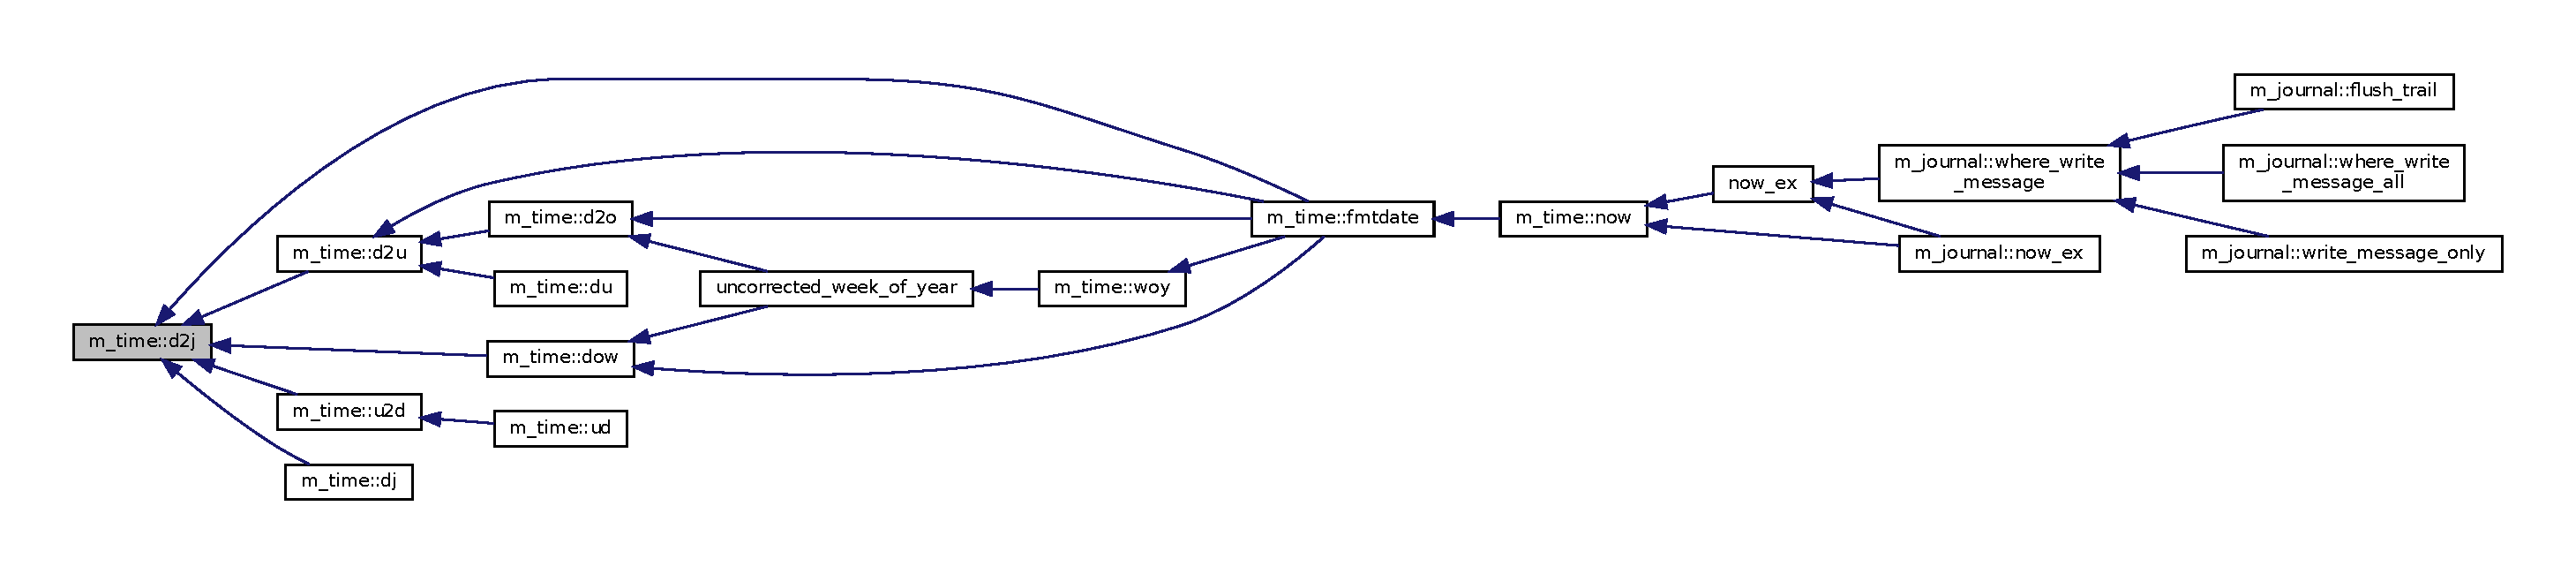
\includegraphics[width=350pt]{namespacem__time_a12cbfe4ebed008f4cdf88df4358df8ad_icgraph}
\end{center}
\end{figure}
\mbox{\Hypertarget{namespacem__time_a727dd77bbd4a5d0e3947c5d303845947}\label{namespacem__time_a727dd77bbd4a5d0e3947c5d303845947}} 
\index{m\+\_\+time@{m\+\_\+time}!d2o@{d2o}}
\index{d2o@{d2o}!m\+\_\+time@{m\+\_\+time}}
\subsubsection{\texorpdfstring{d2o()}{d2o()}}
{\footnotesize\ttfamily integer function, public m\+\_\+time\+::d2o (\begin{DoxyParamCaption}\item[{integer, dimension(8), intent(in)}]{dat }\end{DoxyParamCaption})}



References d2u(), and secday.

Here is the call graph for this function\+:\nopagebreak
\begin{figure}[H]
\begin{center}
\leavevmode
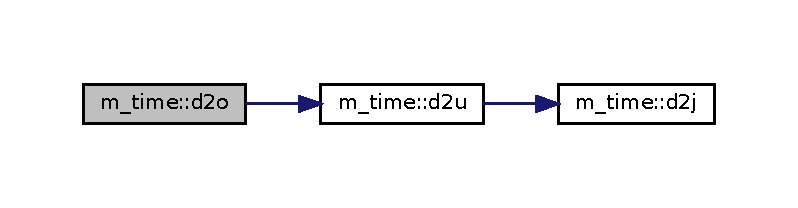
\includegraphics[width=350pt]{namespacem__time_a727dd77bbd4a5d0e3947c5d303845947_cgraph}
\end{center}
\end{figure}
Here is the caller graph for this function\+:\nopagebreak
\begin{figure}[H]
\begin{center}
\leavevmode
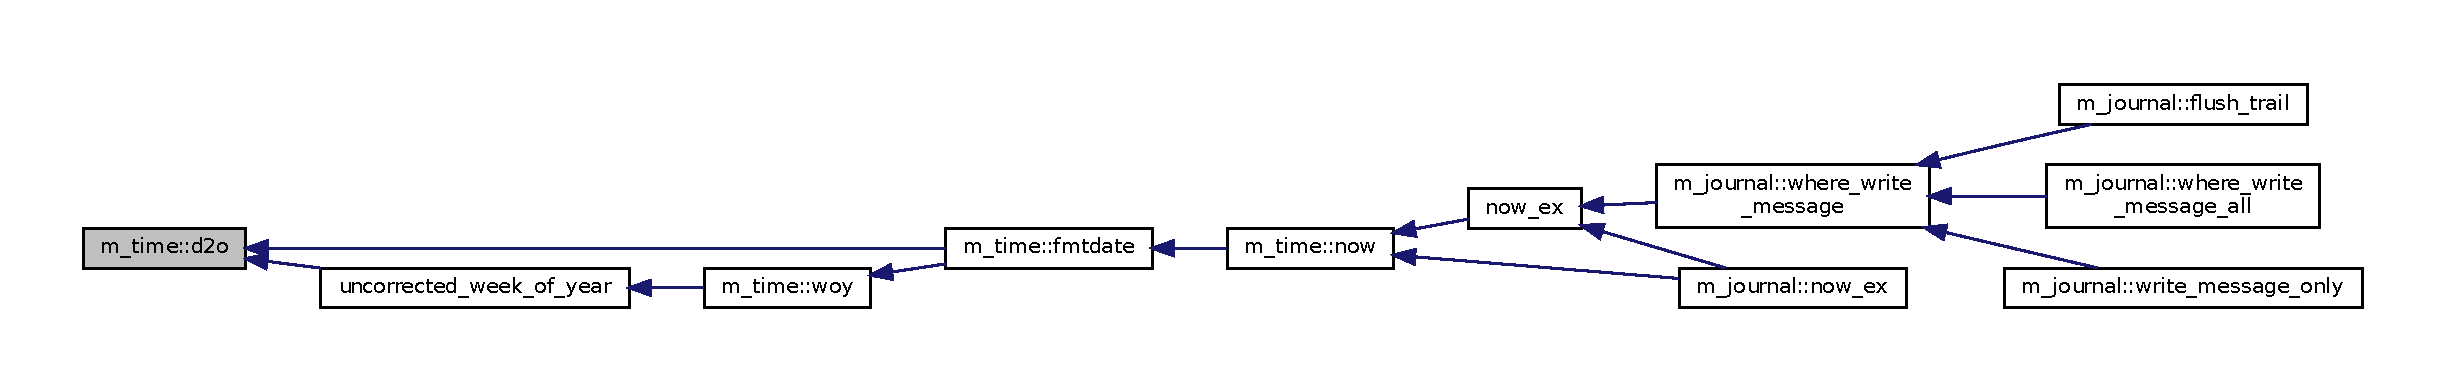
\includegraphics[width=350pt]{namespacem__time_a727dd77bbd4a5d0e3947c5d303845947_icgraph}
\end{center}
\end{figure}
\mbox{\Hypertarget{namespacem__time_ac4bd98688e1277ab6cfc16697331406c}\label{namespacem__time_ac4bd98688e1277ab6cfc16697331406c}} 
\index{m\+\_\+time@{m\+\_\+time}!d2u@{d2u}}
\index{d2u@{d2u}!m\+\_\+time@{m\+\_\+time}}
\subsubsection{\texorpdfstring{d2u()}{d2u()}}
{\footnotesize\ttfamily subroutine, public m\+\_\+time\+::d2u (\begin{DoxyParamCaption}\item[{integer, dimension(8), intent(in)}]{dat,  }\item[{real(kind=\mbox{\hyperlink{namespacem__time_a95f16e7435244d114f0a451625dc189a}{dp}}), intent(out)}]{unixtime,  }\item[{integer, intent(out)}]{ierr }\end{DoxyParamCaption})}



References d2j(), and secday.

Here is the call graph for this function\+:\nopagebreak
\begin{figure}[H]
\begin{center}
\leavevmode
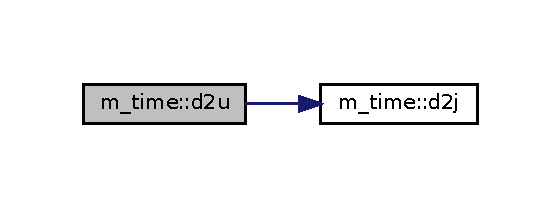
\includegraphics[width=269pt]{namespacem__time_ac4bd98688e1277ab6cfc16697331406c_cgraph}
\end{center}
\end{figure}
Here is the caller graph for this function\+:\nopagebreak
\begin{figure}[H]
\begin{center}
\leavevmode
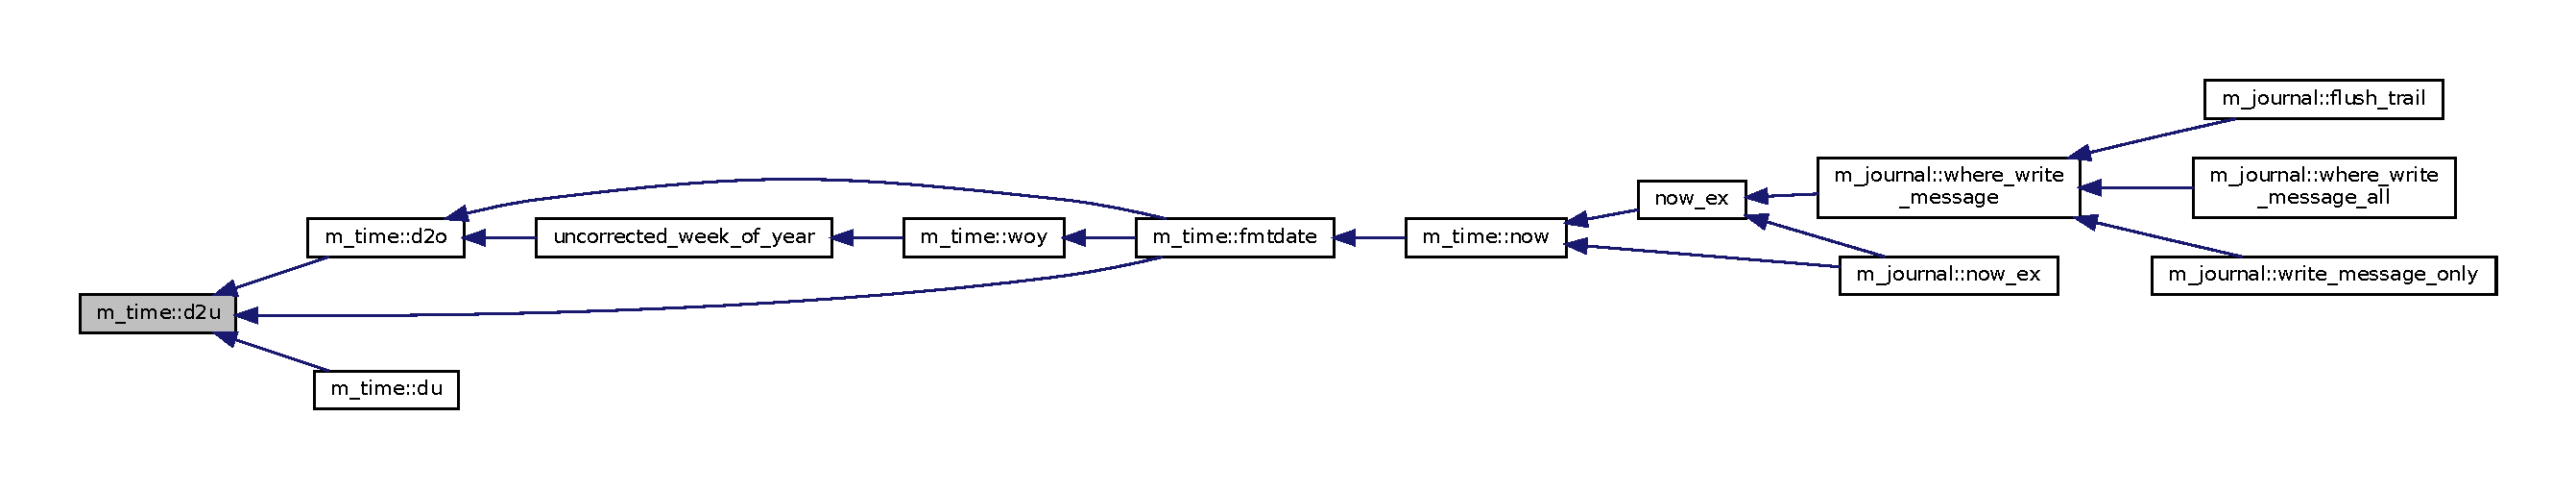
\includegraphics[width=350pt]{namespacem__time_ac4bd98688e1277ab6cfc16697331406c_icgraph}
\end{center}
\end{figure}
\mbox{\Hypertarget{namespacem__time_ad3ce73217cd51090b52a0468b045c0f3}\label{namespacem__time_ad3ce73217cd51090b52a0468b045c0f3}} 
\index{m\+\_\+time@{m\+\_\+time}!dj@{dj}}
\index{dj@{dj}!m\+\_\+time@{m\+\_\+time}}
\subsubsection{\texorpdfstring{dj()}{dj()}}
{\footnotesize\ttfamily real(kind=\mbox{\hyperlink{namespacem__time_a95f16e7435244d114f0a451625dc189a}{dp}}) function, public m\+\_\+time\+::dj (\begin{DoxyParamCaption}\item[{integer, dimension(8), intent(in)}]{dat }\end{DoxyParamCaption})}



References d2j().

Here is the call graph for this function\+:\nopagebreak
\begin{figure}[H]
\begin{center}
\leavevmode
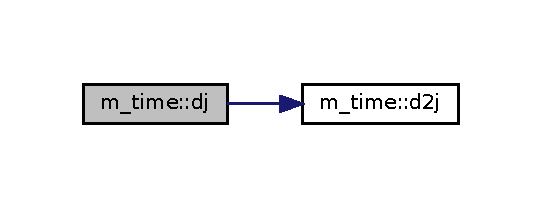
\includegraphics[width=260pt]{namespacem__time_ad3ce73217cd51090b52a0468b045c0f3_cgraph}
\end{center}
\end{figure}
\mbox{\Hypertarget{namespacem__time_adfda8a89820b8d0ad4581a14896e4ce5}\label{namespacem__time_adfda8a89820b8d0ad4581a14896e4ce5}} 
\index{m\+\_\+time@{m\+\_\+time}!dow@{dow}}
\index{dow@{dow}!m\+\_\+time@{m\+\_\+time}}
\subsubsection{\texorpdfstring{dow()}{dow()}}
{\footnotesize\ttfamily subroutine, public m\+\_\+time\+::dow (\begin{DoxyParamCaption}\item[{integer, dimension(8), intent(in)}]{values,  }\item[{integer, intent(out), optional}]{weekday,  }\item[{character$\ast$($\ast$), intent(out), optional}]{day,  }\item[{integer, intent(out)}]{ierr }\end{DoxyParamCaption})}



References d2j().

Here is the call graph for this function\+:\nopagebreak
\begin{figure}[H]
\begin{center}
\leavevmode
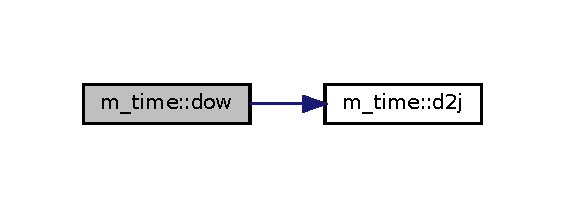
\includegraphics[width=271pt]{namespacem__time_adfda8a89820b8d0ad4581a14896e4ce5_cgraph}
\end{center}
\end{figure}
Here is the caller graph for this function\+:\nopagebreak
\begin{figure}[H]
\begin{center}
\leavevmode
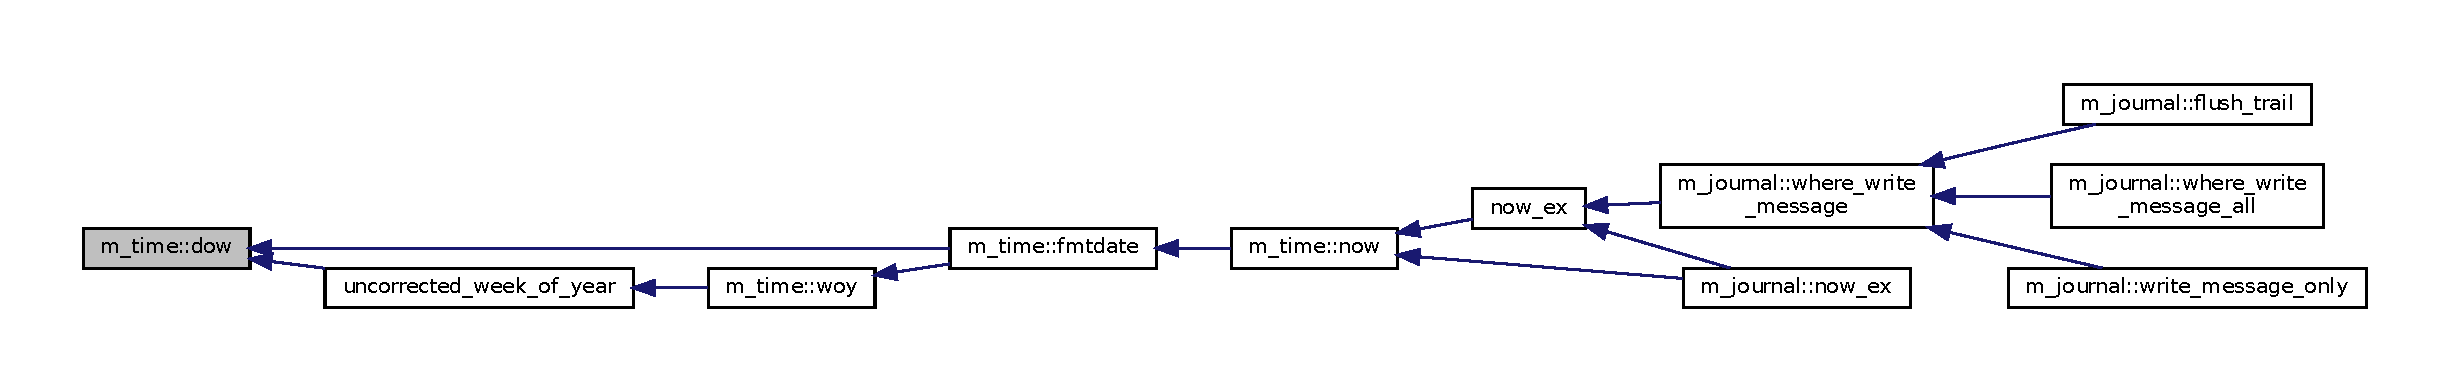
\includegraphics[width=350pt]{namespacem__time_adfda8a89820b8d0ad4581a14896e4ce5_icgraph}
\end{center}
\end{figure}
\mbox{\Hypertarget{namespacem__time_af1b675ed3256cd2ac10d461b8f1c7da8}\label{namespacem__time_af1b675ed3256cd2ac10d461b8f1c7da8}} 
\index{m\+\_\+time@{m\+\_\+time}!du@{du}}
\index{du@{du}!m\+\_\+time@{m\+\_\+time}}
\subsubsection{\texorpdfstring{du()}{du()}}
{\footnotesize\ttfamily real(kind=\mbox{\hyperlink{namespacem__time_a95f16e7435244d114f0a451625dc189a}{dp}}) function, public m\+\_\+time\+::du (\begin{DoxyParamCaption}\item[{integer, dimension(8), intent(in)}]{dat }\end{DoxyParamCaption})}



References d2u().

Here is the call graph for this function\+:\nopagebreak
\begin{figure}[H]
\begin{center}
\leavevmode
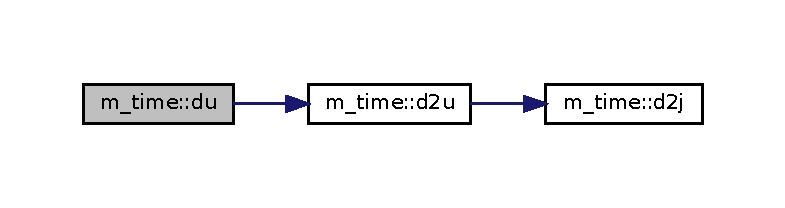
\includegraphics[width=350pt]{namespacem__time_af1b675ed3256cd2ac10d461b8f1c7da8_cgraph}
\end{center}
\end{figure}
\mbox{\Hypertarget{namespacem__time_a2cb84c9b8af4f395b76aed76e1431328}\label{namespacem__time_a2cb84c9b8af4f395b76aed76e1431328}} 
\index{m\+\_\+time@{m\+\_\+time}!fmtdate@{fmtdate}}
\index{fmtdate@{fmtdate}!m\+\_\+time@{m\+\_\+time}}
\subsubsection{\texorpdfstring{fmtdate()}{fmtdate()}}
{\footnotesize\ttfamily character(len=\+:) function, allocatable, public m\+\_\+time\+::fmtdate (\begin{DoxyParamCaption}\item[{integer, dimension(8), intent(in)}]{values,  }\item[{character(len=$\ast$), intent(in)}]{format }\end{DoxyParamCaption})}



References d2j(), d2o(), d2u(), dow(), v2mo(), and woy().

Here is the call graph for this function\+:\nopagebreak
\begin{figure}[H]
\begin{center}
\leavevmode
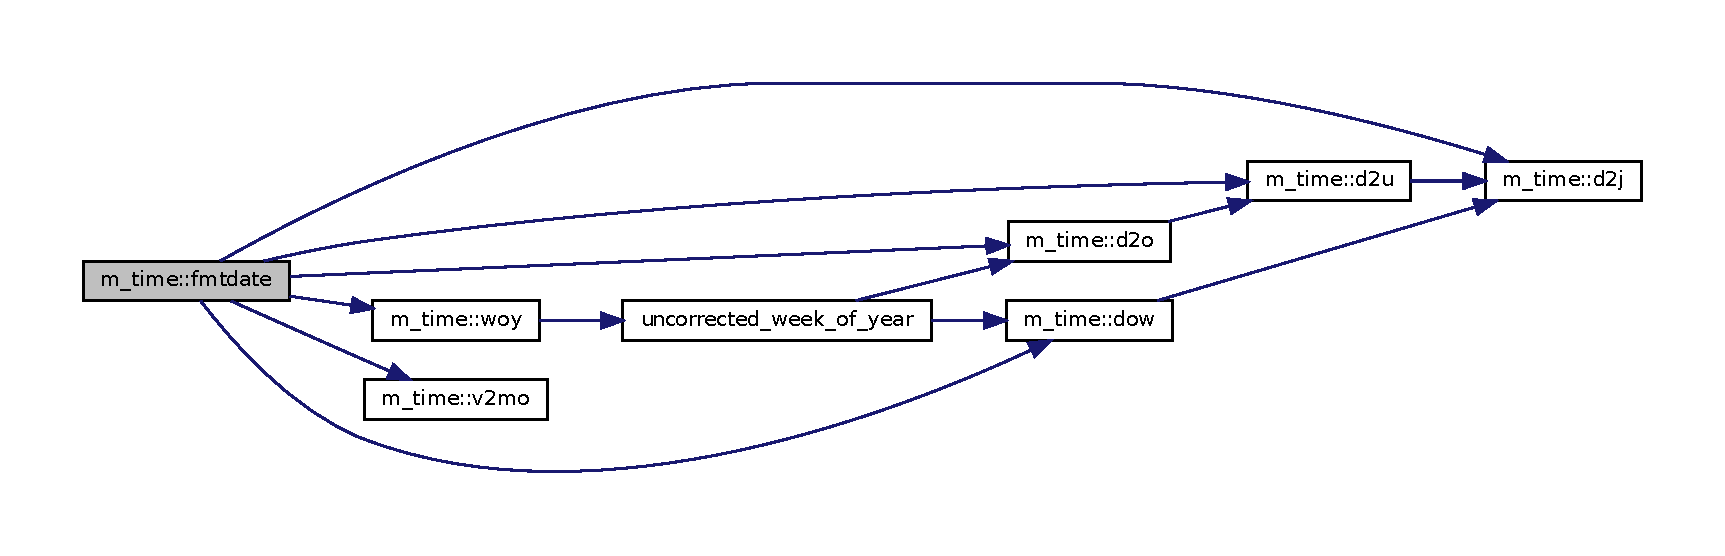
\includegraphics[width=350pt]{namespacem__time_a2cb84c9b8af4f395b76aed76e1431328_cgraph}
\end{center}
\end{figure}
Here is the caller graph for this function\+:\nopagebreak
\begin{figure}[H]
\begin{center}
\leavevmode
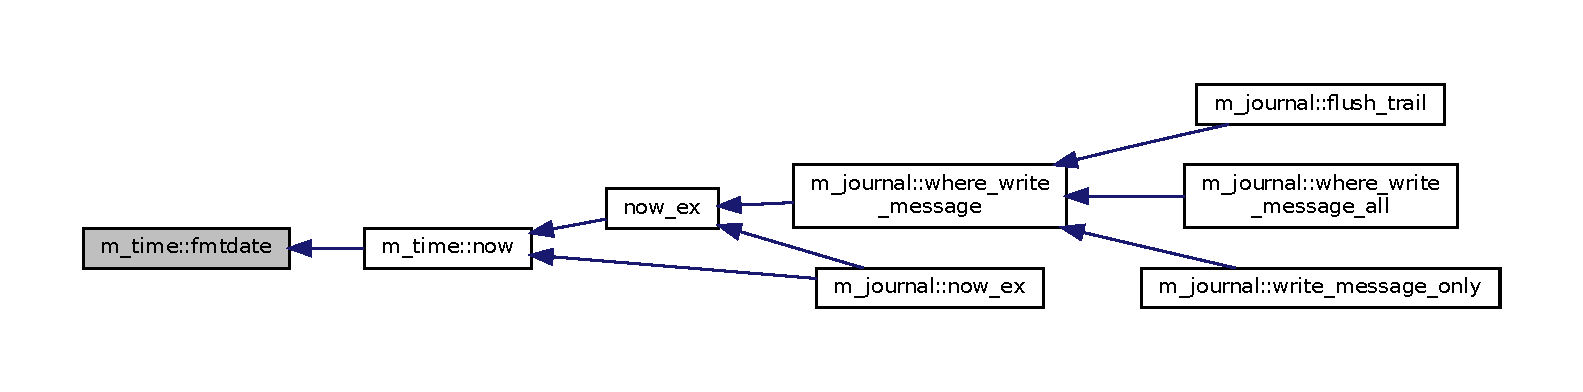
\includegraphics[width=350pt]{namespacem__time_a2cb84c9b8af4f395b76aed76e1431328_icgraph}
\end{center}
\end{figure}
\mbox{\Hypertarget{namespacem__time_a0ec30ca32f18ec409bbbef046a9e73f0}\label{namespacem__time_a0ec30ca32f18ec409bbbef046a9e73f0}} 
\index{m\+\_\+time@{m\+\_\+time}!fmtdate\+\_\+usage@{fmtdate\+\_\+usage}}
\index{fmtdate\+\_\+usage@{fmtdate\+\_\+usage}!m\+\_\+time@{m\+\_\+time}}
\subsubsection{\texorpdfstring{fmtdate\+\_\+usage()}{fmtdate\_usage()}}
{\footnotesize\ttfamily subroutine, public m\+\_\+time\+::fmtdate\+\_\+usage (\begin{DoxyParamCaption}\item[{integer}]{ii }\end{DoxyParamCaption})}

\mbox{\Hypertarget{namespacem__time_a4da84079c6587a8aaa8ef32169a84cc5}\label{namespacem__time_a4da84079c6587a8aaa8ef32169a84cc5}} 
\index{m\+\_\+time@{m\+\_\+time}!j2d@{j2d}}
\index{j2d@{j2d}!m\+\_\+time@{m\+\_\+time}}
\subsubsection{\texorpdfstring{j2d()}{j2d()}}
{\footnotesize\ttfamily subroutine, public m\+\_\+time\+::j2d (\begin{DoxyParamCaption}\item[{integer, dimension(8), intent(out)}]{dat,  }\item[{real(kind=\mbox{\hyperlink{namespacem__time_a95f16e7435244d114f0a451625dc189a}{dp}}), intent(in)}]{julian,  }\item[{integer, intent(out)}]{ierr }\end{DoxyParamCaption})}



References jd(), and secday.

Here is the call graph for this function\+:\nopagebreak
\begin{figure}[H]
\begin{center}
\leavevmode
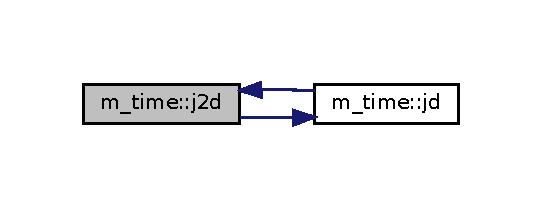
\includegraphics[width=260pt]{namespacem__time_a4da84079c6587a8aaa8ef32169a84cc5_cgraph}
\end{center}
\end{figure}
Here is the caller graph for this function\+:\nopagebreak
\begin{figure}[H]
\begin{center}
\leavevmode
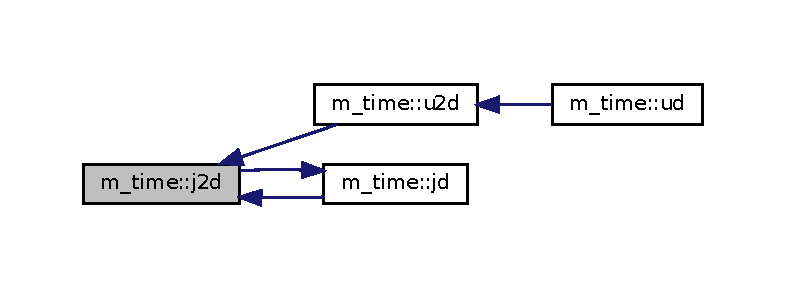
\includegraphics[width=350pt]{namespacem__time_a4da84079c6587a8aaa8ef32169a84cc5_icgraph}
\end{center}
\end{figure}
\mbox{\Hypertarget{namespacem__time_a6c3297c41c6f58f8139c48466a37f292}\label{namespacem__time_a6c3297c41c6f58f8139c48466a37f292}} 
\index{m\+\_\+time@{m\+\_\+time}!jd@{jd}}
\index{jd@{jd}!m\+\_\+time@{m\+\_\+time}}
\subsubsection{\texorpdfstring{jd()}{jd()}}
{\footnotesize\ttfamily integer function, dimension(8), public m\+\_\+time\+::jd (\begin{DoxyParamCaption}\item[{real(kind=\mbox{\hyperlink{namespacem__time_a95f16e7435244d114f0a451625dc189a}{dp}}), intent(in)}]{julian }\end{DoxyParamCaption})}



References j2d().

Here is the call graph for this function\+:\nopagebreak
\begin{figure}[H]
\begin{center}
\leavevmode
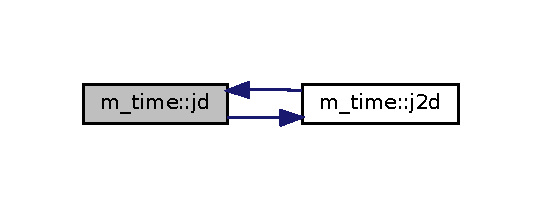
\includegraphics[width=260pt]{namespacem__time_a6c3297c41c6f58f8139c48466a37f292_cgraph}
\end{center}
\end{figure}
Here is the caller graph for this function\+:\nopagebreak
\begin{figure}[H]
\begin{center}
\leavevmode
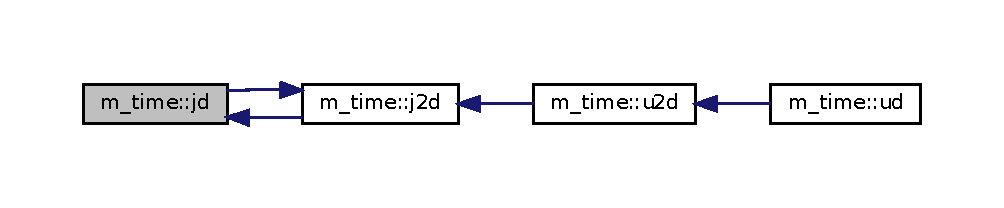
\includegraphics[width=350pt]{namespacem__time_a6c3297c41c6f58f8139c48466a37f292_icgraph}
\end{center}
\end{figure}
\mbox{\Hypertarget{namespacem__time_a6b5e87be0e510ff268c1ecfbf67a3bdb}\label{namespacem__time_a6b5e87be0e510ff268c1ecfbf67a3bdb}} 
\index{m\+\_\+time@{m\+\_\+time}!now@{now}}
\index{now@{now}!m\+\_\+time@{m\+\_\+time}}
\subsubsection{\texorpdfstring{now()}{now()}}
{\footnotesize\ttfamily character(len=\+:) function, allocatable, public m\+\_\+time\+::now (\begin{DoxyParamCaption}\item[{character(len=$\ast$), intent(in), optional}]{format }\end{DoxyParamCaption})}



References fmtdate().

Here is the call graph for this function\+:\nopagebreak
\begin{figure}[H]
\begin{center}
\leavevmode
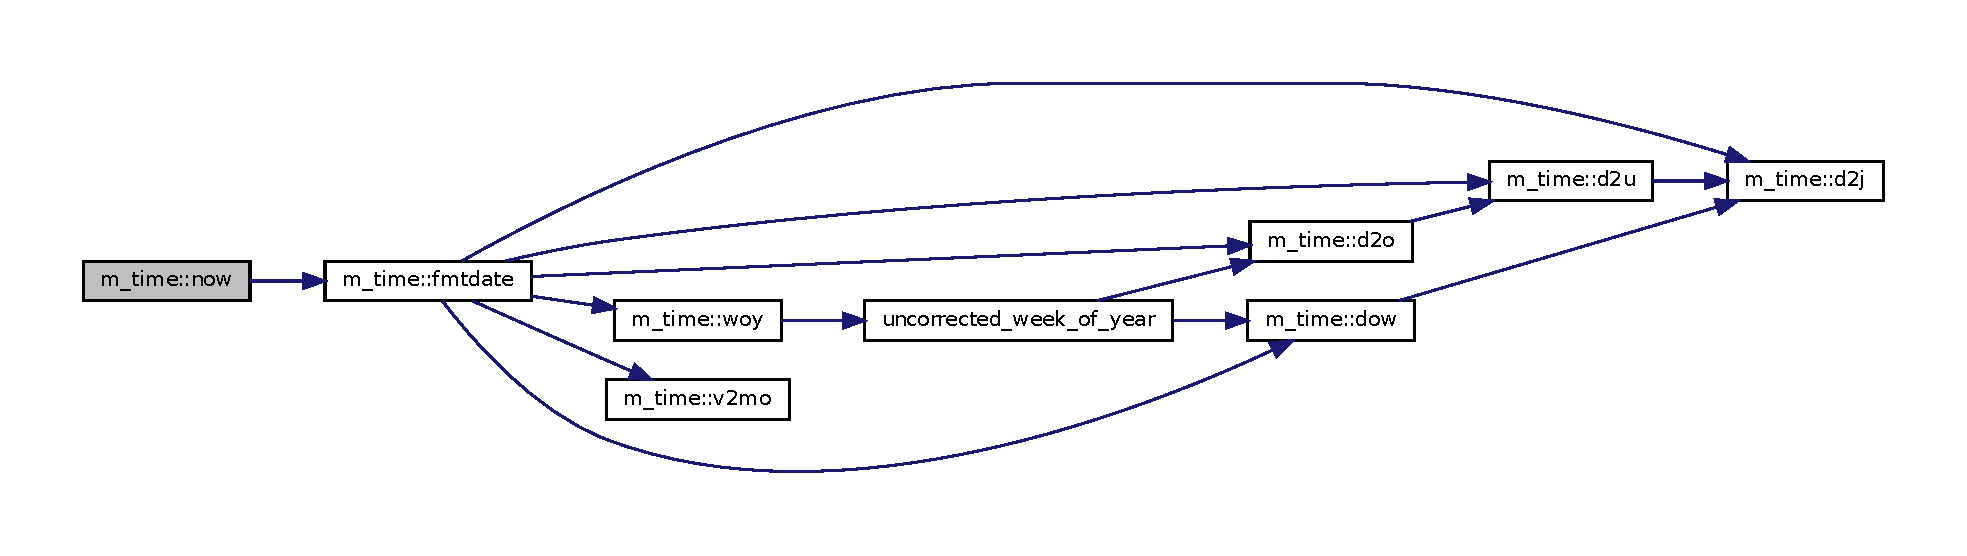
\includegraphics[width=350pt]{namespacem__time_a6b5e87be0e510ff268c1ecfbf67a3bdb_cgraph}
\end{center}
\end{figure}
Here is the caller graph for this function\+:\nopagebreak
\begin{figure}[H]
\begin{center}
\leavevmode
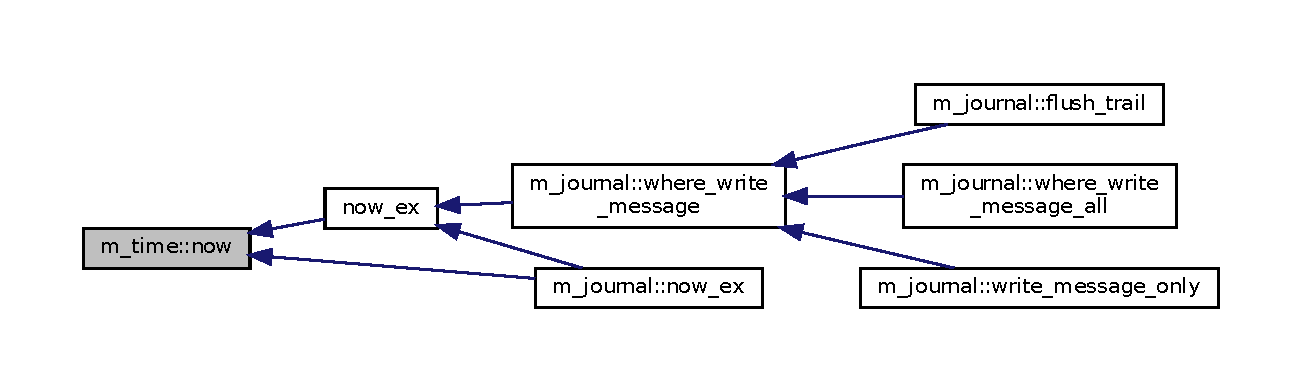
\includegraphics[width=350pt]{namespacem__time_a6b5e87be0e510ff268c1ecfbf67a3bdb_icgraph}
\end{center}
\end{figure}
\mbox{\Hypertarget{namespacem__time_aeb65659c500dd201910f3615858f9b73}\label{namespacem__time_aeb65659c500dd201910f3615858f9b73}} 
\index{m\+\_\+time@{m\+\_\+time}!sys\+\_\+sleep@{sys\+\_\+sleep}}
\index{sys\+\_\+sleep@{sys\+\_\+sleep}!m\+\_\+time@{m\+\_\+time}}
\subsubsection{\texorpdfstring{sys\+\_\+sleep()}{sys\_sleep()}}
{\footnotesize\ttfamily subroutine, public m\+\_\+time\+::sys\+\_\+sleep (\begin{DoxyParamCaption}\item[{integer (c\+\_\+int)}]{wait\+\_\+seconds }\end{DoxyParamCaption})}

\mbox{\Hypertarget{namespacem__time_a6c01c810eb2acce767d2f24b9aaefa56}\label{namespacem__time_a6c01c810eb2acce767d2f24b9aaefa56}} 
\index{m\+\_\+time@{m\+\_\+time}!u2d@{u2d}}
\index{u2d@{u2d}!m\+\_\+time@{m\+\_\+time}}
\subsubsection{\texorpdfstring{u2d()}{u2d()}}
{\footnotesize\ttfamily subroutine, public m\+\_\+time\+::u2d (\begin{DoxyParamCaption}\item[{integer, dimension(8), intent(out)}]{dat,  }\item[{real(kind=\mbox{\hyperlink{namespacem__time_a95f16e7435244d114f0a451625dc189a}{dp}}), intent(in)}]{unixtime,  }\item[{integer, intent(out)}]{ierr }\end{DoxyParamCaption})}



References d2j(), j2d(), and secday.

Here is the call graph for this function\+:\nopagebreak
\begin{figure}[H]
\begin{center}
\leavevmode
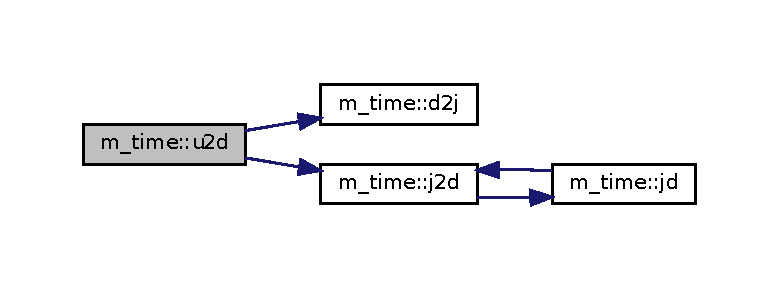
\includegraphics[width=350pt]{namespacem__time_a6c01c810eb2acce767d2f24b9aaefa56_cgraph}
\end{center}
\end{figure}
Here is the caller graph for this function\+:\nopagebreak
\begin{figure}[H]
\begin{center}
\leavevmode
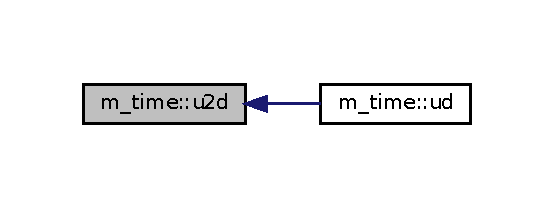
\includegraphics[width=266pt]{namespacem__time_a6c01c810eb2acce767d2f24b9aaefa56_icgraph}
\end{center}
\end{figure}
\mbox{\Hypertarget{namespacem__time_a8b2c0ede467ef5185d478a072a9f969f}\label{namespacem__time_a8b2c0ede467ef5185d478a072a9f969f}} 
\index{m\+\_\+time@{m\+\_\+time}!ud@{ud}}
\index{ud@{ud}!m\+\_\+time@{m\+\_\+time}}
\subsubsection{\texorpdfstring{ud()}{ud()}}
{\footnotesize\ttfamily integer function, dimension(8), public m\+\_\+time\+::ud (\begin{DoxyParamCaption}\item[{real(kind=\mbox{\hyperlink{namespacem__time_a95f16e7435244d114f0a451625dc189a}{dp}}), intent(in)}]{unixtime }\end{DoxyParamCaption})}



References u2d().

Here is the call graph for this function\+:\nopagebreak
\begin{figure}[H]
\begin{center}
\leavevmode
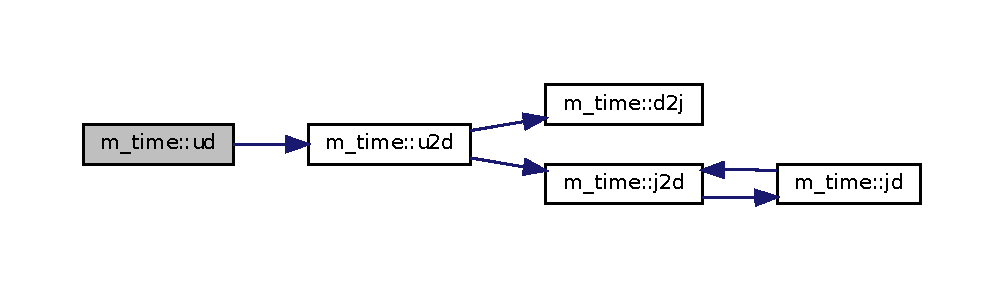
\includegraphics[width=350pt]{namespacem__time_a8b2c0ede467ef5185d478a072a9f969f_cgraph}
\end{center}
\end{figure}
\mbox{\Hypertarget{namespacem__time_a6f28cf00e4998bb50bb503f5e4bd3f77}\label{namespacem__time_a6f28cf00e4998bb50bb503f5e4bd3f77}} 
\index{m\+\_\+time@{m\+\_\+time}!v2mo@{v2mo}}
\index{v2mo@{v2mo}!m\+\_\+time@{m\+\_\+time}}
\subsubsection{\texorpdfstring{v2mo()}{v2mo()}}
{\footnotesize\ttfamily character(len=\+:) function, allocatable, public m\+\_\+time\+::v2mo (\begin{DoxyParamCaption}\item[{integer, intent(in)}]{imonth }\end{DoxyParamCaption})}

Here is the caller graph for this function\+:\nopagebreak
\begin{figure}[H]
\begin{center}
\leavevmode
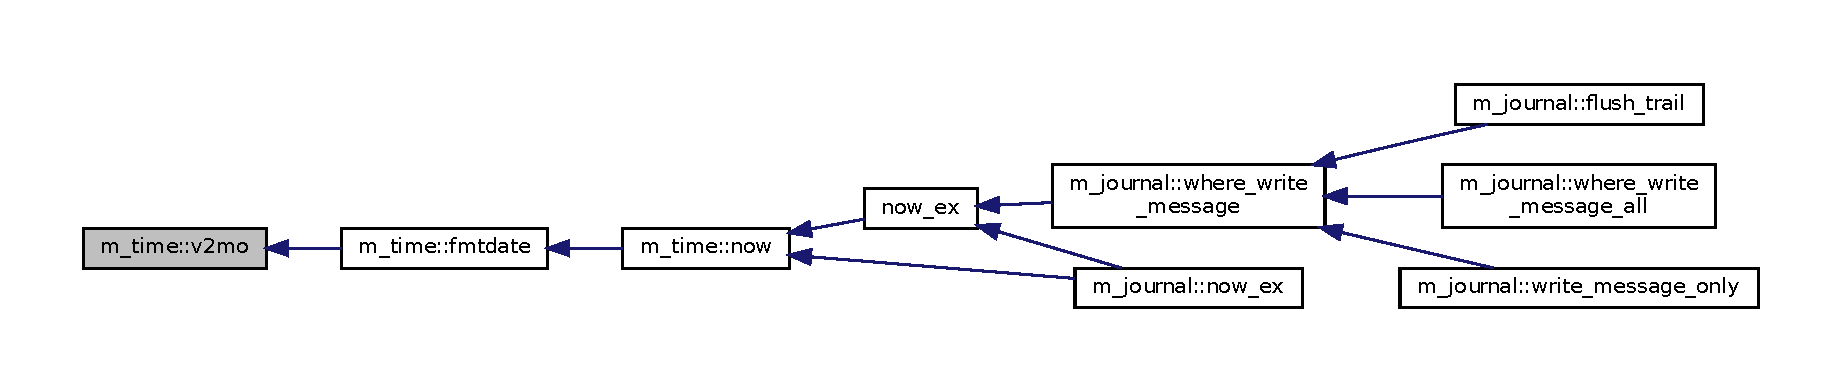
\includegraphics[width=350pt]{namespacem__time_a6f28cf00e4998bb50bb503f5e4bd3f77_icgraph}
\end{center}
\end{figure}
\mbox{\Hypertarget{namespacem__time_aea9216971a364d79beb307f36e9e3873}\label{namespacem__time_aea9216971a364d79beb307f36e9e3873}} 
\index{m\+\_\+time@{m\+\_\+time}!woy@{woy}}
\index{woy@{woy}!m\+\_\+time@{m\+\_\+time}}
\subsubsection{\texorpdfstring{woy()}{woy()}}
{\footnotesize\ttfamily subroutine, public m\+\_\+time\+::woy (\begin{DoxyParamCaption}\item[{integer, dimension(8), intent(in)}]{dat,  }\item[{integer, intent(out)}]{iso\+\_\+year,  }\item[{integer, intent(out)}]{iso\+\_\+week,  }\item[{integer, intent(out)}]{iso\+\_\+weekday,  }\item[{character(len=10), intent(out)}]{iso\+\_\+name }\end{DoxyParamCaption})}



References uncorrected\+\_\+week\+\_\+of\+\_\+year().

Here is the call graph for this function\+:\nopagebreak
\begin{figure}[H]
\begin{center}
\leavevmode
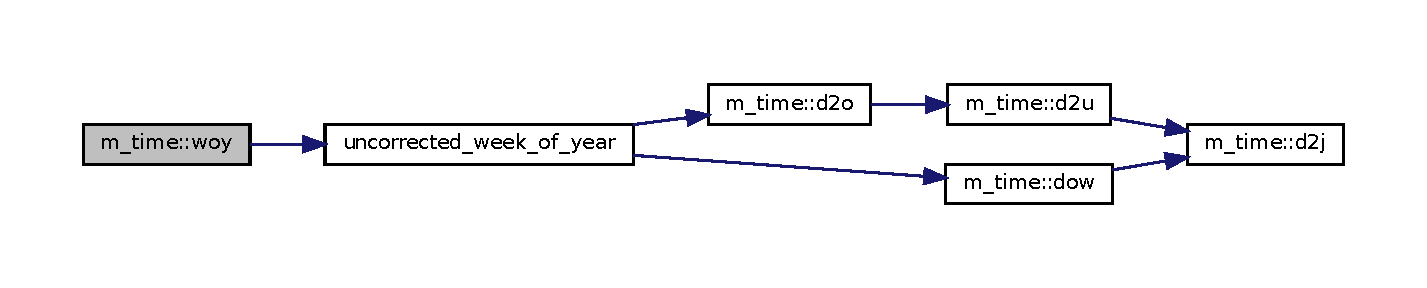
\includegraphics[width=350pt]{namespacem__time_aea9216971a364d79beb307f36e9e3873_cgraph}
\end{center}
\end{figure}
Here is the caller graph for this function\+:\nopagebreak
\begin{figure}[H]
\begin{center}
\leavevmode
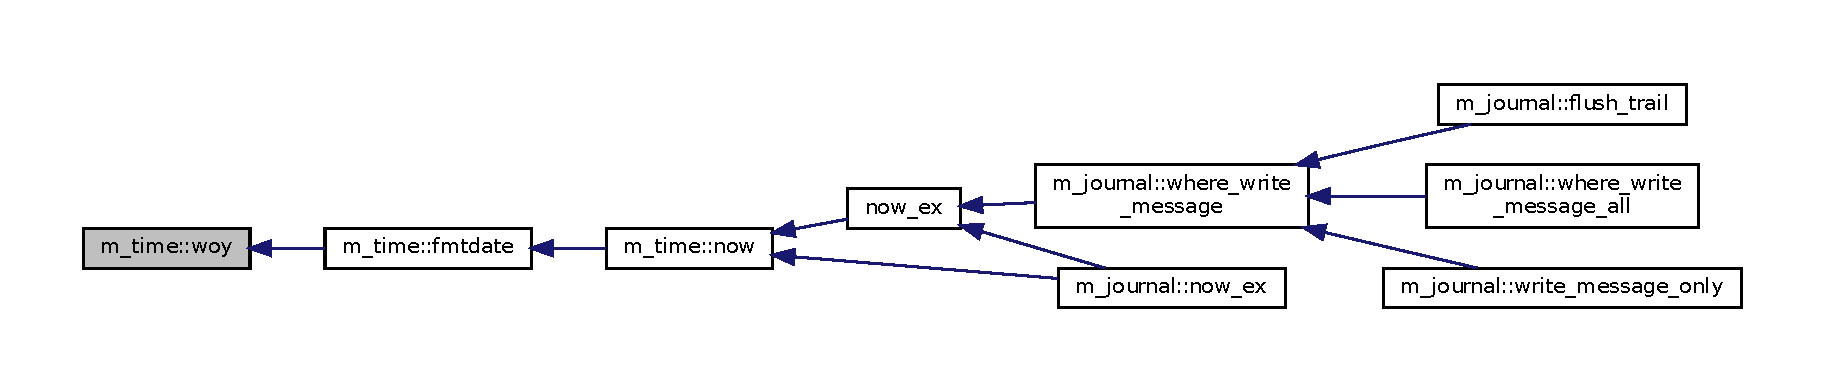
\includegraphics[width=350pt]{namespacem__time_aea9216971a364d79beb307f36e9e3873_icgraph}
\end{center}
\end{figure}


\subsection{Variable Documentation}
\mbox{\Hypertarget{namespacem__time_a95f16e7435244d114f0a451625dc189a}\label{namespacem__time_a95f16e7435244d114f0a451625dc189a}} 
\index{m\+\_\+time@{m\+\_\+time}!dp@{dp}}
\index{dp@{dp}!m\+\_\+time@{m\+\_\+time}}
\subsubsection{\texorpdfstring{dp}{dp}}
{\footnotesize\ttfamily integer, parameter, private m\+\_\+time\+::dp =kind(0.\+0d0)\hspace{0.3cm}{\ttfamily [private]}}

\mbox{\Hypertarget{namespacem__time_a2c21a39cf2aa1f48e7f03d3542c0fab2}\label{namespacem__time_a2c21a39cf2aa1f48e7f03d3542c0fab2}} 
\index{m\+\_\+time@{m\+\_\+time}!secday@{secday}}
\index{secday@{secday}!m\+\_\+time@{m\+\_\+time}}
\subsubsection{\texorpdfstring{secday}{secday}}
{\footnotesize\ttfamily real(kind=\mbox{\hyperlink{namespacem__time_a95f16e7435244d114f0a451625dc189a}{dp}}) m\+\_\+time\+::secday =86400.\+0d0\hspace{0.3cm}{\ttfamily [private]}}


\hypertarget{namespacem__verify}{}\section{m\+\_\+verify Module Reference}
\label{namespacem__verify}\index{m\+\_\+verify@{m\+\_\+verify}}


\subsubsection*{N\+A\+ME}

M\+\_\+verify(3fm) -\/ \mbox{[}M\+\_\+verify\mbox{]} a collection of Fortran routines for supporting code development by providing error processing, debugging procedures and unit testing. (L\+I\+C\+E\+N\+SE\+:PD) \subsubsection*{S\+Y\+N\+O\+P\+S\+IS} 


\subsection*{Functions/\+Subroutines}
\begin{DoxyCompactItemize}
\item 
subroutine, public \mbox{\hyperlink{namespacem__verify_a74ea8b4574606c4f72e97b115375fc9b}{unit\+\_\+check\+\_\+msg}} (name, g1, g2, g3, g4, g5, g6, g7, g8, g9)
\begin{DoxyCompactList}\small\item\em \subsubsection*{N\+A\+ME}

unit\+\_\+check\+\_\+msg(3f) -\/ \mbox{[}M\+\_\+verify\mbox{]} converts up to nine standard scalar values to a message for unit testing (L\+I\+C\+E\+N\+SE\+:PD) \subsubsection*{S\+Y\+N\+O\+P\+S\+IS}\end{DoxyCompactList}\item 
subroutine, public \mbox{\hyperlink{namespacem__verify_a41f795f932767c97b5ef481a694f4f84}{stderr}} (msg, gen0, gen1, gen2, gen3, gen4, gen5, gen6, gen7, gen8, gen9)
\begin{DoxyCompactList}\small\item\em \subsubsection*{N\+A\+ME}

stderr(3f) -\/ \mbox{[}M\+\_\+verify\mbox{]} write message to stderr (L\+I\+C\+E\+N\+SE\+:PD) \subsubsection*{S\+Y\+N\+O\+P\+S\+IS}\end{DoxyCompactList}\item 
subroutine, public \mbox{\hyperlink{namespacem__verify_a2695833d468118d68918d6aeabab6d0b}{fstop}} (ierr, stdout, \mbox{\hyperlink{namespacem__verify_a41f795f932767c97b5ef481a694f4f84}{stderr}})
\begin{DoxyCompactList}\small\item\em \subsubsection*{N\+A\+ME}

fstop(3f) -\/ \mbox{[}M\+\_\+verify\mbox{]} call stop with both a number and a message (L\+I\+C\+E\+N\+SE\+:PD) \subsubsection*{S\+Y\+N\+O\+P\+S\+IS}\end{DoxyCompactList}\item 
subroutine, public \mbox{\hyperlink{namespacem__verify_a96149da1a302f2a157d79dadc94e755e}{unit\+\_\+check}} (name, logical\+\_\+expression, msg, msg1, msg2, msg3, msg4, msg5, msg6, msg7, msg8, msg9)
\begin{DoxyCompactList}\small\item\em \subsubsection*{N\+A\+ME}

unit\+\_\+check(3f) -\/ \mbox{[}M\+\_\+verify\mbox{]} if logical expression is false, call command \char`\"{}goodbad N\+A\+M\+E bad\char`\"{} and stop program by default (L\+I\+C\+E\+N\+SE\+:PD) \end{DoxyCompactList}\item 
subroutine, public \mbox{\hyperlink{namespacem__verify_ad753d0a58dbc02c8917bf2b2aa3e1de7}{unit\+\_\+check\+\_\+start}} (name, options, msg)
\begin{DoxyCompactList}\small\item\em \subsubsection*{N\+A\+ME}

unit\+\_\+check\+\_\+start(3f) -\/ \mbox{[}M\+\_\+verify\mbox{]} call command \char`\"{}goodbad N\+A\+M\+E start\char`\"{} and optionally set options (L\+I\+C\+E\+N\+SE\+:PD) \end{DoxyCompactList}\item 
subroutine, public \mbox{\hyperlink{namespacem__verify_a0c0ed723b61b2cbbebb81fa91edd1941}{unit\+\_\+check\+\_\+done}} (name, opts, msg)
\begin{DoxyCompactList}\small\item\em \subsubsection*{N\+A\+ME}

unit\+\_\+check\+\_\+done(3f) -\/ \mbox{[}M\+\_\+verify\mbox{]} call command \char`\"{}goodbad N\+A\+M\+E good\char`\"{} or \char`\"{}goodbad N\+A\+M\+E bad\char`\"{} depending on whether failures were found (L\+I\+C\+E\+N\+SE\+:PD) \end{DoxyCompactList}\item 
subroutine, public \mbox{\hyperlink{namespacem__verify_aaa2744e5ab1687072183869bd53cc086}{unit\+\_\+check\+\_\+bad}} (name, opts, msg)
\begin{DoxyCompactList}\small\item\em \subsubsection*{N\+A\+ME}

unit\+\_\+check\+\_\+bad(3f) -\/ \mbox{[}M\+\_\+verify\mbox{]} call command \char`\"{}goodbad N\+A\+M\+E bad\char`\"{} and stop program (L\+I\+C\+E\+N\+SE\+:PD) \end{DoxyCompactList}\item 
subroutine, public \mbox{\hyperlink{namespacem__verify_a9d5ed59a1ac977dd7ab23e0d1fb54de4}{unit\+\_\+check\+\_\+good}} (name, opts, msg)
\begin{DoxyCompactList}\small\item\em \subsubsection*{N\+A\+ME}

unit\+\_\+check\+\_\+good(3f) -\/ \mbox{[}M\+\_\+verify\mbox{]} call command \char`\"{}goodbad N\+A\+M\+E good\char`\"{} (L\+I\+C\+E\+N\+SE\+:PD) \end{DoxyCompactList}\item 
subroutine, public \mbox{\hyperlink{namespacem__verify_aa772ce395fd2e4cc546b8645d8fd9949}{pdec}} (string)
\begin{DoxyCompactList}\small\item\em \subsubsection*{N\+A\+ME}

pdec(3f) -\/ \mbox{[}M\+\_\+verify\mbox{]} write out string with A\+S\+C\+II decimal equivalent vertically under it (L\+I\+C\+E\+N\+SE\+:PD) \end{DoxyCompactList}\item 
function \mbox{\hyperlink{namespacem__verify_a6185c00609b8f0e4c5a503cfadcb2490}{atleast}} (line, length)
\item 
subroutine, public \mbox{\hyperlink{namespacem__verify_a83a6bafddb101d8b0fe70f34827836ff}{assert}} (filename, linen, expr, g1, g2, g3, g4, g5, g6, g7, g8, g9)
\begin{DoxyCompactList}\small\item\em \subsubsection*{N\+A\+ME}

assert(3f) -\/ \mbox{[}M\+\_\+verify\mbox{]} print filename, linenumber, and message to stderr and stop program (L\+I\+C\+E\+N\+SE\+:PD) \subsubsection*{S\+Y\+N\+O\+P\+S\+IS}\end{DoxyCompactList}\item 
real(kind=\mbox{\hyperlink{namespacem__verify_a7f6aa94b09b3824bc5c15bc74e757d6b}{realtime}}) function \mbox{\hyperlink{namespacem__verify_a1a97667eb1d53ce5b97a60c4a9ebe565}{julian}} ()
\item 
logical function, public \mbox{\hyperlink{namespacem__verify_ac5b0a0323929702a4b9e3fb918ea19b3}{almost}} (x, y, digits, verbose)
\begin{DoxyCompactList}\small\item\em \subsubsection*{N\+A\+ME}

almost(3f) -\/ \mbox{[}M\+\_\+verify\mbox{]} return true or false if two numbers agree up to specified number of digits (L\+I\+C\+E\+N\+SE\+:PD) \subsubsection*{S\+Y\+N\+O\+P\+S\+IS}\end{DoxyCompactList}\item 
subroutine, public \mbox{\hyperlink{namespacem__verify_a311d01ea90882e4db1e87520ba731d5c}{accdig}} (X, Y, digi0, A\+C\+U\+R\+CY, I\+ND)
\begin{DoxyCompactList}\small\item\em \subsubsection*{N\+A\+ME}

accdig(3f) -\/ \mbox{[}M\+\_\+verify\mbox{]} compare two real numbers only up to a specified number of digits (L\+I\+C\+E\+N\+SE\+:PD) \end{DoxyCompactList}\item 
subroutine, public \mbox{\hyperlink{namespacem__verify_a7408df33e6934a8959fdeda8cc3fb5ff}{dp\+\_\+accdig}} (x, y, digi0, A\+C\+U\+R\+CY, I\+ND)
\begin{DoxyCompactList}\small\item\em \subsubsection*{N\+A\+ME}

dp\+\_\+accdig(3f) -\/ \mbox{[}M\+\_\+verify\mbox{]} compare two numbers only up to a specified number of digits (L\+I\+C\+E\+N\+SE\+:PD) \end{DoxyCompactList}\item 
elemental pure logical function, public \mbox{\hyperlink{namespacem__verify_aa0d8de1c26ca3aae0366b9fb8ead21c4}{in\+\_\+margin}} (expected\+\_\+value, measured\+\_\+value, allowed\+\_\+margin)
\begin{DoxyCompactList}\small\item\em \subsubsection*{N\+A\+ME}

in\+\_\+margin(3f) -\/ \mbox{[}M\+\_\+verify\mbox{]} check if two reals are approximately equal using a relative margin \end{DoxyCompactList}\item 
real(kind=dp) function, public \mbox{\hyperlink{namespacem__verify_af997c802e1ad966d55f023822b2f645a}{round}} (val, idigits0)
\item 
pure elemental real(kind=real128) function \mbox{\hyperlink{namespacem__verify_ab08d7bdca3b5d5e99732919be5880dc4}{anyscalar\+\_\+to\+\_\+real128}} (valuein)
\item 
pure elemental doubleprecision function \mbox{\hyperlink{namespacem__verify_a92278514bcbb93fefca1d925e3dfba65}{anyscalar\+\_\+to\+\_\+double}} (valuein)
\end{DoxyCompactItemize}
\subsection*{Variables}
\begin{DoxyCompactItemize}
\item 
integer, save, public \mbox{\hyperlink{namespacem__verify_a7014b3aa584eb29266bf52fc6e03e6ed}{io\+\_\+debug}} =E\+R\+R\+O\+R\+\_\+\+U\+N\+IT
\item 
integer, save, public \mbox{\hyperlink{namespacem__verify_a65569c8b4be204251ba14430ad18372d}{unit\+\_\+check\+\_\+lun}} =E\+R\+R\+O\+R\+\_\+\+U\+N\+IT
\item 
logical, save, public \mbox{\hyperlink{namespacem__verify_a0f87b43bebf70897f9ec711be3f01839}{debug}} =.false.
\item 
logical, save, public \mbox{\hyperlink{namespacem__verify_a434af7c4d380da5b85d49dc07466dde8}{unit\+\_\+check\+\_\+keep\+\_\+going}} =.false.
\item 
integer, save, public \mbox{\hyperlink{namespacem__verify_afe37222ddb2a9470e1a0e9c40e2dcce3}{unit\+\_\+check\+\_\+level}} =0
\item 
character(len=4096), public \mbox{\hyperlink{namespacem__verify_aaa3c6dfa94a9414592071525036020d4}{unit\+\_\+check\+\_\+command}} =\textquotesingle{}goodbad\textquotesingle{}
\item 
integer, parameter, public \mbox{\hyperlink{namespacem__verify_a7f6aa94b09b3824bc5c15bc74e757d6b}{realtime}} =kind(0.\+0d0)
\item 
integer, parameter, public \mbox{\hyperlink{namespacem__verify_a278d7a36f55fac875e4f94bc893447fe}{exit\+\_\+success}} =0
\item 
integer, parameter, public \mbox{\hyperlink{namespacem__verify_a458c47b6b47738f8ebadddb4a944d0e0}{exit\+\_\+failure}} =1
\item 
real(kind=\mbox{\hyperlink{namespacem__verify_a7f6aa94b09b3824bc5c15bc74e757d6b}{realtime}}), save \mbox{\hyperlink{namespacem__verify_a77729c599fbd8aed6075a05fb3c38146}{duration}} =0.\+0d0
\item 
integer, save \mbox{\hyperlink{namespacem__verify_af97c7f92394811bec5fed506fdfab67d}{clicks}} =0.\+0d0
\item 
logical, save \mbox{\hyperlink{namespacem__verify_a425cad68370e8552495e1838b2e34734}{stop\+\_\+g}} =.true.
\item 
integer, save \mbox{\hyperlink{namespacem__verify_ada62999b3a1ef795c335deccac28cda5}{ipassed\+\_\+g}} =0
\item 
integer, save \mbox{\hyperlink{namespacem__verify_ab18f1875be62b6aa1e101894358b617f}{ifailed\+\_\+g}} =0
\item 
logical, save, public \mbox{\hyperlink{namespacem__verify_aa827fd6225334c65efe89d1d0af79efa}{no\+\_\+news\+\_\+is\+\_\+good\+\_\+news}} =.false.
\end{DoxyCompactItemize}


\subsection{Detailed Description}
\subsubsection*{N\+A\+ME}

M\+\_\+verify(3fm) -\/ \mbox{[}M\+\_\+verify\mbox{]} a collection of Fortran routines for supporting code development by providing error processing, debugging procedures and unit testing. (L\+I\+C\+E\+N\+SE\+:PD) \subsubsection*{S\+Y\+N\+O\+P\+S\+IS}

use M\+\_\+verify, only \+: unit\+\_\+check, unit\+\_\+check\+\_\+start, unit\+\_\+check\+\_\+good, unit\+\_\+check\+\_\+bad, unit\+\_\+check\+\_\+done use M\+\_\+verify, only \+: unit\+\_\+check\+\_\+limit, unit\+\_\+check\+\_\+keep\+\_\+going, unit\+\_\+check\+\_\+command use M\+\_\+verify, only \+: unit\+\_\+check\+\_\+msg use M\+\_\+verify, only \+: debug use M\+\_\+verify, only \+: fstop use M\+\_\+verify, only \+: stderr use M\+\_\+verify, only \+: assert

\subsubsection*{Q\+U\+O\+TE}

Do not let your victories go to your head, nor let your failures go to your heart.

\subsubsection*{D\+E\+S\+C\+R\+I\+P\+T\+I\+ON}

The M\+\_\+verify(3fm) Fortran module provides procedures and variables useful for providing error processing, debugging capabilities, and unit testing.

o allows for a user-\/defined command to be called to collect results or mail failure alerts, ... o supports easily composing a message from up to nine scalar intrinsic values and different message levels o allows stopping on first failure or continuing

S\+ET M\+O\+D\+ES unit\+\_\+check\+\_\+keep\+\_\+going logical variable that can be used to turn off program termination on errors. unit\+\_\+check\+\_\+level An integer that can be used to specify different debug levels unit\+\_\+check\+\_\+command name of command to execute. Defaults to the name \char`\"{}goodbad\char`\"{}. U\+N\+IT T\+E\+S\+TS unit\+\_\+check\+\_\+start(3f) start tests of a procedure and optionally call \begin{DoxyVerb}                      command NAME start ..."
\end{DoxyVerb}
 unit\+\_\+check(3f) if expression is false optionally call \begin{DoxyVerb}                      command NAME bad
                   and stop program (by default)
\end{DoxyVerb}


unit\+\_\+check\+\_\+done(3f) call \begin{DoxyVerb}                      command NAME good
                   if no failures
                   else call
                      command NAME bad
\end{DoxyVerb}
 unit\+\_\+check\+\_\+good(3f) call command command N\+A\+ME good unit\+\_\+check\+\_\+bad(3f) call command command N\+A\+ME bad and stop program by default unit\+\_\+check\+\_\+msg(3f) write message

B\+A\+S\+IC D\+E\+B\+U\+G\+G\+I\+NG fstop(3f) calls \textquotesingle{}S\+T\+OP V\+A\+L\+UE\textquotesingle{} passing in a value (1-\/32), with optional message pdec(3f) write A\+S\+C\+II Decimal Equivalent (A\+DE) numbers vertically beneath string stderr(3f) Write message on stderr debug logical variable that can be tested by routines as a flag to process debug statements.

For unit testing, the existence of a command called \char`\"{}goodbad\char`\"{} is initially assumed. This is generally a script that makes entries for each unit in an S\+Q\+Lite data file which is then used to create C\+SV and H\+T\+ML reports on the status of each unit. A sample goodbad(1) command written in the bash(1) shell and using the sqlite3(1) command should be included in this distribution as an example

The flexibility introduced by calling an external script or program is that The goodbad(1) command can be changed as desired to write C\+SV files or simple logs or to notify developers with e-\/mail as desired.

R\+E\+L\+A\+T\+ED F\+U\+N\+C\+T\+I\+O\+NS

The routines in M\+\_\+verify(3f) are often combined with the M\+\_\+hashkeys(3fm) routines and various math and statistical routines to quickly create unit tests.

Comparisons of real values can be done with a tolerance with M\+\_\+\+Compare\+\_\+\+Float\+\_\+\+Numbers(3fm), for example.

The intrinsics A\+N\+Y(3f) and A\+L\+L(3f) are particularly useful in calls to unit\+\_\+check(3f).

\subsubsection*{E\+X\+A\+M\+P\+L\+ES}

Sample program

!!program demo\+\_\+unit\+\_\+tests module M\+\_\+demo private public one !! regular routines public two !! regular routines public test\+\_\+suite\+\_\+\+M\+\_\+demo !! special name for use with test\+\_\+suite(1bash). contains

!! regular routines subroutine one() end subroutine one

subroutine two() end subroutine two

!! unit test subroutine test\+\_\+suite\+\_\+\+M\+\_\+demo use M\+\_\+verify, only\+: unit\+\_\+check\+\_\+start, unit\+\_\+check use M\+\_\+verify, only\+: unit\+\_\+check\+\_\+good, unit\+\_\+check\+\_\+bad, unit\+\_\+check\+\_\+done use M\+\_\+verify, only\+: unit\+\_\+check\+\_\+msg implicit none integer \+:\+: i, j, k integer,allocatable \+:\+: array(\+:) integer \+:\+: arr(4)=\mbox{[}21,51,14,45\mbox{]} integer \+:\+: a=21, b=51, c=14, d=45 ! T\+E\+S\+T-\/\+D\+R\+I\+V\+EN D\+E\+V\+E\+L\+O\+P\+M\+E\+NT ! optional set-\/up perform initialization operations common to all tests within a module i=1 j=2 k=3 array=\mbox{[}10,20,30,40,50,60,70\mbox{]} call test\+\_\+one() call test\+\_\+two() ! optional tear-\/down perform finalization operations common to all tests within a module contains

subroutine test\+\_\+one() ! register an entry for specified name (\char`\"{}one\char`\"{}) in database with status of zero (0) call unit\+\_\+check\+\_\+start(\textquotesingle{}one\textquotesingle{})

! if mask test fails, can ! $\ast$ produce a S\+U\+C\+C\+E\+SS\+: or F\+A\+IL\+: message and stop program ! $\ast$ change database status for specified entry to -\/1 and stop program, else continue ! $\ast$ produce a S\+U\+C\+C\+E\+SS\+: or F\+A\+IL\+: message and keep going ! $\ast$ produce a F\+A\+IL\+: message if test fails but no S\+U\+C\+C\+E\+SS\+: message if test passes call unit\+\_\+check(\textquotesingle{}one\textquotesingle{},i.\+gt.\+0,msg=\textquotesingle{}I $>$ 0\textquotesingle{})

! using A\+N\+Y(3f) and A\+L\+L(3f) call unit\+\_\+check(\textquotesingle{}one\textquotesingle{},all(\mbox{[}i,j,k\mbox{]}.gt.\+0), \textquotesingle{}testing if everyone greater than zero\textquotesingle{}) ! display message built of scalars as well call unit\+\_\+check(\textquotesingle{}one\textquotesingle{},all(.not.\mbox{[}i,j,k\mbox{]}.eq.\+4),\textquotesingle{}for set \textquotesingle{},i,j,k,\textquotesingle{}testing if no one is equal to four\textquotesingle{})

! for tests that are hard to reduce to a logical test just call unit\+\_\+check\+\_\+bad(3f) if fail if(i+j+k.lt.\+1)then call unit\+\_\+check\+\_\+bad(\textquotesingle{}one\textquotesingle{}) endif

call unit\+\_\+check\+\_\+done(\textquotesingle{}one\textquotesingle{},\textquotesingle{}checks on \char`\"{}one\char`\"{} ended\textquotesingle{}) end subroutine test\+\_\+one

subroutine test\+\_\+two ! use of all(3f), any(3f), merge(3f) can be useful ! if you know what these would produce ! write($\ast$,$\ast$)\mbox{[}\textquotesingle{}A\textquotesingle{},\textquotesingle{}X\textquotesingle{},\textquotesingle{}X\textquotesingle{},\textquotesingle{}X\textquotesingle{},\textquotesingle{}X\textquotesingle{},\textquotesingle{}B\textquotesingle{}\mbox{]}.eq.\textquotesingle{}B\textquotesingle{} ! this would return an array, the last element having the value T, else F ! write($\ast$,$\ast$)all(\mbox{[}\textquotesingle{}A\textquotesingle{},\textquotesingle{}X\textquotesingle{},\textquotesingle{}X\textquotesingle{},\textquotesingle{}X\textquotesingle{},\textquotesingle{}X\textquotesingle{},\textquotesingle{}X\textquotesingle{}\mbox{]}.eq.\textquotesingle{}X\textquotesingle{}) ! this would return F ! write($\ast$,$\ast$)any(\mbox{[}\textquotesingle{}A\textquotesingle{},\textquotesingle{}X\textquotesingle{},\textquotesingle{}X\textquotesingle{},\textquotesingle{}X\textquotesingle{},\textquotesingle{}X\textquotesingle{},\textquotesingle{}X\textquotesingle{}\mbox{]}.eq.\textquotesingle{}B\textquotesingle{}) ! this would return F ! write($\ast$,$\ast$)any(\mbox{[}\textquotesingle{}A\textquotesingle{},\textquotesingle{}X\textquotesingle{},\textquotesingle{}X\textquotesingle{},\textquotesingle{}X\textquotesingle{},\textquotesingle{}X\textquotesingle{},\textquotesingle{}B\textquotesingle{}\mbox{]}.eq.\textquotesingle{}B\textquotesingle{}) ! this would return T ! write($\ast$,$\ast$).not.\+all(array.\+lt.\+100) ! write($\ast$,$\ast$)all(array.\+lt.\+100) ! write($\ast$,$\ast$)all(\mbox{[}a,b,c,d\mbox{]}.eq.\mbox{[}21,51,14,45\mbox{]}) ! compare a list. This would return T ! write($\ast$,$\ast$)all(arr.\+eq.\mbox{[}21,51,14,45\mbox{]}) ! compare an array. This would return T ! you know how valuable A\+N\+Y(3f) and A\+L\+L(3f) will be call unit\+\_\+check\+\_\+start(\textquotesingle{}two\textquotesingle{},\textquotesingle{}check on \char`\"{}two\char`\"{} passed\textquotesingle{}) call unit\+\_\+check(\textquotesingle{}two\textquotesingle{}, 1.\+gt.\+0 .and. abs(10.\+10000-\/10.\+10001).lt.\+0.\+0001,msg=\textquotesingle{}two looks good\textquotesingle{}) call unit\+\_\+check\+\_\+done(\textquotesingle{}two\textquotesingle{},\textquotesingle{}checks on \char`\"{}two\char`\"{} ended\textquotesingle{}) end subroutine test\+\_\+two

end subroutine test\+\_\+suite\+\_\+\+M\+\_\+demo

end module M\+\_\+demo

program demo\+\_\+\+M\+\_\+verify use M\+\_\+demo, only\+: test\+\_\+suite\+\_\+\+M\+\_\+demo use M\+\_\+verify, only\+: unit\+\_\+check\+\_\+command, unit\+\_\+check\+\_\+keep\+\_\+going,unit\+\_\+check\+\_\+level unit\+\_\+check\+\_\+command=\textquotesingle{}\textquotesingle{} unit\+\_\+check\+\_\+keep\+\_\+going=.true. unit\+\_\+check\+\_\+level=0 call test\+\_\+suite\+\_\+\+M\+\_\+demo end program demo\+\_\+\+M\+\_\+verify

Expected output\+:

unit\+\_\+check\+: one S\+U\+C\+C\+E\+SS\+:I $>$ 0 unit\+\_\+check\+: one S\+U\+C\+C\+E\+SS\+:testing if everyone greater than zero unit\+\_\+check\+: one S\+U\+C\+C\+E\+SS\+:for set 1 2 3 testing if no one is equal to four unit\+\_\+check\+\_\+done\+: one P\+A\+S\+S\+ED G\+O\+OD\+:3 B\+AD\+:0

unit\+\_\+check\+: two S\+U\+C\+C\+E\+SS\+:two looks good unit\+\_\+check\+\_\+done\+: two P\+A\+S\+S\+ED G\+O\+OD\+:1 B\+AD\+:0

\subsubsection*{A\+U\+T\+H\+OR}

John S. Urban \subsubsection*{L\+I\+C\+E\+N\+SE}

Public Domain 

\subsection{Function/\+Subroutine Documentation}
\mbox{\Hypertarget{namespacem__verify_a311d01ea90882e4db1e87520ba731d5c}\label{namespacem__verify_a311d01ea90882e4db1e87520ba731d5c}} 
\index{m\+\_\+verify@{m\+\_\+verify}!accdig@{accdig}}
\index{accdig@{accdig}!m\+\_\+verify@{m\+\_\+verify}}
\subsubsection{\texorpdfstring{accdig()}{accdig()}}
{\footnotesize\ttfamily subroutine, public m\+\_\+verify\+::accdig (\begin{DoxyParamCaption}\item[{real, intent(in)}]{X,  }\item[{real, intent(in)}]{Y,  }\item[{real, intent(in)}]{digi0,  }\item[{real, intent(out)}]{A\+C\+U\+R\+CY,  }\item[{integer, intent(out)}]{I\+ND }\end{DoxyParamCaption})}



\subsubsection*{N\+A\+ME}

accdig(3f) -\/ \mbox{[}M\+\_\+verify\mbox{]} compare two real numbers only up to a specified number of digits (L\+I\+C\+E\+N\+SE\+:PD) 

\subsubsection*{S\+Y\+N\+O\+P\+S\+IS}

\begin{DoxyVerb}   subroutine accdig(x,y,digio,acurcy,ind)

    real,intent(in)     :: X
    real,intent(in)     :: Y
    real,intent(in)     :: DIGI0
    real,intent(out)    :: acurcy
    integer,intent(out) :: ind
\end{DoxyVerb}


\subsubsection*{D\+E\+S\+C\+R\+I\+P\+T\+I\+ON}

This procedure is used to check how closely two numbers agree.

call accdig(\+X,\+Y,\+D\+I\+G\+I0,\+A\+C\+U\+R\+C\+Y,\+I\+N\+D)

The values X and Y are the numbers to compare, and D\+I\+G\+I0 is the threshold number of digits to consider significant in returning I\+ND.

If X and Y are considered equal within D\+I\+G\+I0 relative tolerance, \begin{DoxyVerb}IND    = 0, if tolerance is     satisfied.
       = 1, if tolerance is not satisfied.
\end{DoxyVerb}


The result A\+C\+U\+R\+CY gives a measure of the number of leading digits in X which are the same as the number of leading digits in Y. \begin{DoxyVerb}    ACURCY=-log10((X-Y)/Y)   if X != Y and Y != 0
    ACURCY=-log10(X-Y)       if X != Y and Y = 0
    ACURCY=8                 if X=Y

    ACURCY is never less than -8 or greater than 8
\end{DoxyVerb}


T\+O\+L\+E\+R\+A\+N\+CE ... X and Y are considered equal within D\+I\+G\+I0 relative tolerance, if A\+C\+U\+R\+CY is greater than D\+I\+G\+I0.

For example, Take some numbers and compare then to 1.\+2345678 ... 

 A number $\vert$ A\+C\+U\+R\+CY $\vert$ A\+C\+U\+R\+CY \subsection*{$\vert$ 1.\+2345678=Y $\vert$ 1.\+2345678=X }

1.\+234680 $\vert$ 3.\+7900571 $\vert$ 3.\+7901275 1.\+2345378 $\vert$ 4.\+6144510 $\vert$ 4.\+6144404 2.\+2234568 $\vert$ 0.\+096367393 $\vert$ 0.\+35188114 1.\+2345678 $\vert$ 8.\+0000000 $\vert$ 8.\+0000000 1.\+2345679 $\vert$ 7.\+0732967 $\vert$ 7.\+0731968 -\/1.\+2345678 $\vert$ -\/0.\+30103000 $\vert$ -\/0.\+30103000 76.\+234567 $\vert$ -\/1.\+7835463 $\vert$ 0.\+0070906729 2.\+4691356 $\vert$ 0.\+0 $\vert$ 0.\+3010300 0.\+0 $\vert$ 0.\+0 $\vert$ -\/0.\+91514942.

Due to the typical limits of the log function, the number of significant digits in the result is best considered to be three.

Notice that 1.\+2345678=Y produces different values than 1.\+2345678=X

A negative result indicates the two values being compared either do not agree in the first digit or they differ with respect to sign. An example of two numbers which do not agree in their leading digit (and actually differ in order of magnitude) is given above by X=76.\+234567 and Y=1.\+2345678; the accuracy reported is -\/1.\+7835463. An example of two numbers which do not agree in sign in X=-\/1.\+2345678 and Y=1.\+2345678; here the accuracy reported is -\/0.\+30103000.

\subsubsection*{E\+X\+A\+M\+P\+LE}

Example program\+:

program demo\+\_\+accdig ! fortran 90 example use M\+\_\+verify, only \+: accdig implicit none integer \+:\+: digi integer \+:\+: i10, i20, i30 integer \+:\+: ind, ind1, ind2 real \+:\+: acurcy, acurcy1, acurcy2 real \+:\+: a, b real \+:\+: vals(9) data vals/ \& \&1.\+234680, 1.\+2345378, 2.\+2234568, 1.\+2345678, \& \&1.\+2345679, -\/1.\+2345678, 76.\+234567, 2.\+4691356, \& \&0.\+0/ write($\ast$,$\ast$)\textquotesingle{}=========================\textquotesingle{} do i10=0,16 a=1.\+0 b=a+1.0/(10$\ast$$\ast$i10) call accdig(a,b,8.\+0,acurcy,ind) write($\ast$,$\ast$)i10,a,b,acurcy,ind enddo write($\ast$,$\ast$)\textquotesingle{}=========================\textquotesingle{} digi=16 do i20=0,digi a=1.\+0 b=a+1.0/(10$\ast$$\ast$i20) call accdig(a,b,real(digi),acurcy,ind) write($\ast$,$\ast$)i20,a,b,acurcy,ind enddo write($\ast$,$\ast$)\textquotesingle{}=========================\textquotesingle{} do i30=1,9 call accdig(1.\+2345678,vals(i30),8.\+0,acurcy1,ind1) call accdig(vals(i30),1.\+2345678,8.\+0,acurcy2,ind2) write($\ast$,$\ast$)i30,vals(i30),acurcy1,acurcy2,ind1,ind2 enddo end program demo\+\_\+accdig

\subsubsection*{R\+E\+F\+E\+R\+E\+N\+C\+ES}

based on ...

N\+BS O\+M\+N\+I\+T\+AB 1980 V\+E\+R\+S\+I\+ON 6.\+01 1/ 1/81. accdig V 7.\+00 2/14/90. $\ast$$\ast$ David Hogben, Statistical Engineering Division, Center for Computing and Applied Mathematics, A337 Administration Building, National Institute of Standards and Technology, Gaithersburg, MD 20899 T\+E\+L\+E\+P\+H\+O\+NE 301-\/975-\/2845 O\+R\+I\+G\+I\+N\+AL V\+E\+R\+S\+I\+ON -\/ October, 1969. C\+U\+R\+R\+E\+NT V\+E\+R\+S\+I\+ON -\/ February, 1990. J\+SU V\+E\+R\+S\+I\+ON -\/ February, 1991.

\subsubsection*{D\+E\+P\+E\+N\+D\+E\+N\+C\+I\+ES}

o M\+\_\+journal(),log10(), abs(1)

\subsubsection*{A\+U\+T\+H\+OR}

David Hogben, John S. Urban

\subsubsection*{L\+I\+C\+E\+N\+SE}

Public Domain Here is the caller graph for this function\+:\nopagebreak
\begin{figure}[H]
\begin{center}
\leavevmode
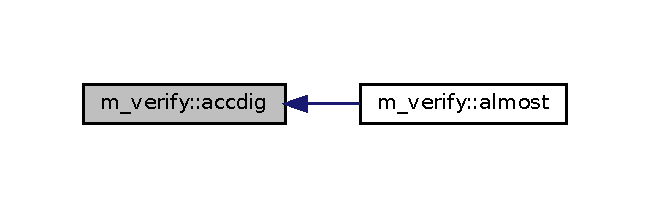
\includegraphics[width=312pt]{namespacem__verify_a311d01ea90882e4db1e87520ba731d5c_icgraph}
\end{center}
\end{figure}
\mbox{\Hypertarget{namespacem__verify_ac5b0a0323929702a4b9e3fb918ea19b3}\label{namespacem__verify_ac5b0a0323929702a4b9e3fb918ea19b3}} 
\index{m\+\_\+verify@{m\+\_\+verify}!almost@{almost}}
\index{almost@{almost}!m\+\_\+verify@{m\+\_\+verify}}
\subsubsection{\texorpdfstring{almost()}{almost()}}
{\footnotesize\ttfamily logical function, public m\+\_\+verify\+::almost (\begin{DoxyParamCaption}\item[{class($\ast$), intent(in)}]{x,  }\item[{class($\ast$), intent(in)}]{y,  }\item[{class($\ast$), intent(in)}]{digits,  }\item[{logical, intent(in), optional}]{verbose }\end{DoxyParamCaption})}



\subsubsection*{N\+A\+ME}

almost(3f) -\/ \mbox{[}M\+\_\+verify\mbox{]} return true or false if two numbers agree up to specified number of digits (L\+I\+C\+E\+N\+SE\+:PD) \subsubsection*{S\+Y\+N\+O\+P\+S\+IS}

function almost(x,y,digits)

class($\ast$),intent(in) \+:\+: x,y class($\ast$),intent(in) \+:\+: rdigits logical,intent(in),optional \+:\+: verbose logical \+:\+: almost

\subsubsection*{D\+E\+S\+C\+R\+I\+P\+T\+I\+ON}

Returns true or false depending on whether the two numbers given agree to within the specified number of digits as calculated by A\+C\+C\+D\+I\+G(3f). \subsubsection*{O\+P\+T\+I\+O\+NS}

x,y expected and calculated values to be compared. May be of type R\+E\+AL, I\+N\+T\+E\+G\+ER, or D\+O\+U\+B\+L\+E\+P\+R\+E\+C\+I\+S\+I\+ON. rdigits real number representing number of digits of precision to compare verbose optional value that specifies to print the results of the comparison when set to .T\+R\+UE.. \subsubsection*{R\+E\+T\+U\+R\+NS}

almost T\+R\+UE if the input values compare up to the specified number of values \subsubsection*{E\+X\+A\+M\+P\+LE}

sample\+:

program demo\+\_\+almost use M\+\_\+verify, only \+: almost real \+:\+: x, y logical \+:\+: z x=1.\+2345678 y=1.\+2300000 do i=1,8 z=almost(x,y,real(i),verbose=.true.) write($\ast$,$\ast$)i,z enddo end program demo\+\_\+almost

output\+:

{\itshape almost} for values 1.\+23456776 1.\+23000002 agreement of 2.\+43020344 digits out of requested 1.\+0 1 T {\itshape almost} for values 1.\+23456776 1.\+23000002 agreement of 2.\+43020344 digits out of requested 2.\+0 2 T {\itshape almost} for values 1.\+23456776 1.\+23000002 agreement of 2.\+43020344 digits out of requested 3.\+0 3 F {\itshape almost} for values 1.\+23456776 1.\+23000002 agreement of 2.\+43020344 digits out of requested 4.\+0 4 F {\itshape almost} for values 1.\+23456776 1.\+23000002 agreement of 2.\+43020344 digits out of requested 5.\+0 5 F {\itshape almost} for values 1.\+23456776 1.\+23000002 agreement of 2.\+43020344 digits out of requested 6.\+0 6 F {\itshape almost} for values 1.\+23456776 1.\+23000002 agreement of 2.\+43020344 digits out of requested 7.\+0 7 F {\itshape accdig} significant digit request too high= 8.\+00000000 {\itshape almost} for values 1.\+23456776 1.\+23000002 agreement of 2.\+43020344 digits out of requested 8.\+0 8 F \subsubsection*{A\+U\+T\+H\+OR}

John S. Urban \subsubsection*{L\+I\+C\+E\+N\+SE}

Public Domain 

References accdig(), anyscalar\+\_\+to\+\_\+real128(), and dp\+\_\+accdig().

Here is the call graph for this function\+:\nopagebreak
\begin{figure}[H]
\begin{center}
\leavevmode
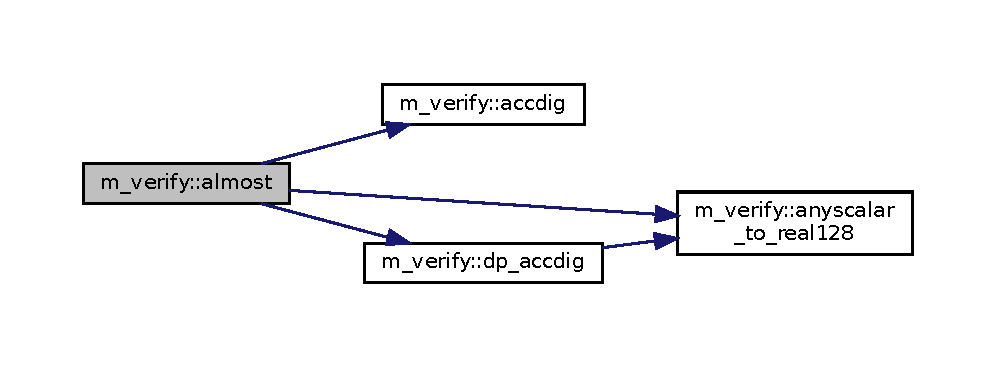
\includegraphics[width=350pt]{namespacem__verify_ac5b0a0323929702a4b9e3fb918ea19b3_cgraph}
\end{center}
\end{figure}
\mbox{\Hypertarget{namespacem__verify_a92278514bcbb93fefca1d925e3dfba65}\label{namespacem__verify_a92278514bcbb93fefca1d925e3dfba65}} 
\index{m\+\_\+verify@{m\+\_\+verify}!anyscalar\+\_\+to\+\_\+double@{anyscalar\+\_\+to\+\_\+double}}
\index{anyscalar\+\_\+to\+\_\+double@{anyscalar\+\_\+to\+\_\+double}!m\+\_\+verify@{m\+\_\+verify}}
\subsubsection{\texorpdfstring{anyscalar\+\_\+to\+\_\+double()}{anyscalar\_to\_double()}}
{\footnotesize\ttfamily pure elemental doubleprecision function m\+\_\+verify\+::anyscalar\+\_\+to\+\_\+double (\begin{DoxyParamCaption}\item[{class($\ast$), intent(in)}]{valuein }\end{DoxyParamCaption})\hspace{0.3cm}{\ttfamily [private]}}

Here is the caller graph for this function\+:\nopagebreak
\begin{figure}[H]
\begin{center}
\leavevmode
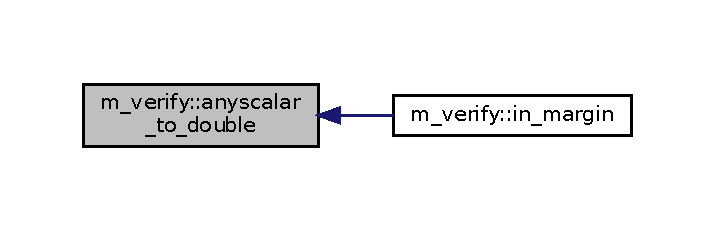
\includegraphics[width=343pt]{namespacem__verify_a92278514bcbb93fefca1d925e3dfba65_icgraph}
\end{center}
\end{figure}
\mbox{\Hypertarget{namespacem__verify_ab08d7bdca3b5d5e99732919be5880dc4}\label{namespacem__verify_ab08d7bdca3b5d5e99732919be5880dc4}} 
\index{m\+\_\+verify@{m\+\_\+verify}!anyscalar\+\_\+to\+\_\+real128@{anyscalar\+\_\+to\+\_\+real128}}
\index{anyscalar\+\_\+to\+\_\+real128@{anyscalar\+\_\+to\+\_\+real128}!m\+\_\+verify@{m\+\_\+verify}}
\subsubsection{\texorpdfstring{anyscalar\+\_\+to\+\_\+real128()}{anyscalar\_to\_real128()}}
{\footnotesize\ttfamily pure elemental real(kind=real128) function m\+\_\+verify\+::anyscalar\+\_\+to\+\_\+real128 (\begin{DoxyParamCaption}\item[{class($\ast$), intent(in)}]{valuein }\end{DoxyParamCaption})\hspace{0.3cm}{\ttfamily [private]}}

Here is the caller graph for this function\+:\nopagebreak
\begin{figure}[H]
\begin{center}
\leavevmode
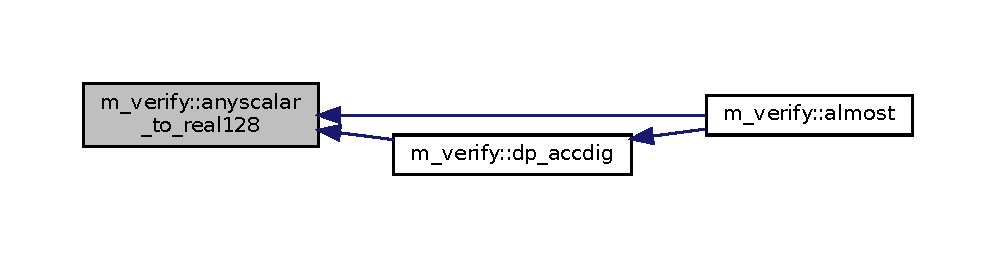
\includegraphics[width=350pt]{namespacem__verify_ab08d7bdca3b5d5e99732919be5880dc4_icgraph}
\end{center}
\end{figure}
\mbox{\Hypertarget{namespacem__verify_a83a6bafddb101d8b0fe70f34827836ff}\label{namespacem__verify_a83a6bafddb101d8b0fe70f34827836ff}} 
\index{m\+\_\+verify@{m\+\_\+verify}!assert@{assert}}
\index{assert@{assert}!m\+\_\+verify@{m\+\_\+verify}}
\subsubsection{\texorpdfstring{assert()}{assert()}}
{\footnotesize\ttfamily subroutine, public m\+\_\+verify\+::assert (\begin{DoxyParamCaption}\item[{character(len=$\ast$), intent(in)}]{filename,  }\item[{integer, intent(in)}]{linen,  }\item[{logical, intent(in)}]{expr,  }\item[{class($\ast$), intent(in), optional}]{g1,  }\item[{class($\ast$), intent(in), optional}]{g2,  }\item[{class($\ast$), intent(in), optional}]{g3,  }\item[{class($\ast$), intent(in), optional}]{g4,  }\item[{class($\ast$), intent(in), optional}]{g5,  }\item[{class($\ast$), intent(in), optional}]{g6,  }\item[{class($\ast$), intent(in), optional}]{g7,  }\item[{class($\ast$), intent(in), optional}]{g8,  }\item[{class($\ast$), intent(in), optional}]{g9 }\end{DoxyParamCaption})}



\subsubsection*{N\+A\+ME}

assert(3f) -\/ \mbox{[}M\+\_\+verify\mbox{]} print filename, linenumber, and message to stderr and stop program (L\+I\+C\+E\+N\+SE\+:PD) \subsubsection*{S\+Y\+N\+O\+P\+S\+IS}

function assert(file,linenum,expr,g1,g2g3,g4,g5,g6,g7,g8,g9)

character(len=$\ast$),intent(in) \+:\+: file character(len=$\ast$),intent(in) \+:\+: linenum logical,intent(in) \+:\+: expr class($\ast$),intent(in),optional \+:\+: g1,g2,g3,g4,g5,g6,g7,g8,g9 \subsubsection*{D\+E\+S\+C\+R\+I\+P\+T\+I\+ON}

assert(3f) prints strings to stderr and then stops program with exit code 1 It labels the first string as the filename, the next integer parameter as the linenumber, and then up to nine scalar values.

It is primarily intended for use by the ufpp(1) preprocessor \$\+A\+S\+S\+E\+RT directive

\subsubsection*{O\+P\+T\+I\+O\+NS}

\begin{DoxyVerb}filename   a string assumed to be the current filename when compiling
linenum    assumed to be the line number of the source code the ASSERT(3f)
           procedure was called at.
expr       logical value
g[1-9]  optional value(s) to print as a message before stopping. May
        be of type INTEGER, LOGICAL, REAL, DOUBLEPRECISION, COMPLEX,
        or CHARACTER.
\end{DoxyVerb}


\subsubsection*{E\+X\+A\+M\+P\+L\+ES}

Sample program\+:

program demo\+\_\+assert use M\+\_\+verify, only \+: assert implicit none character(len=\+:),allocatable \+:\+: pr real \+:\+: a, toobig=1024 a=2000 call assert(\textquotesingle{}myroutine\textquotesingle{}, 101, a.\+gt.\+toobig, \textquotesingle{}The value is too large\textquotesingle{}, a, \textquotesingle{}.gt.\textquotesingle{}, toobig) end program demo\+\_\+assert

\subsubsection*{A\+U\+T\+H\+OR}

John S. Urban \subsubsection*{L\+I\+C\+E\+N\+SE}

Public Domain 

References stderr().

Here is the call graph for this function\+:\nopagebreak
\begin{figure}[H]
\begin{center}
\leavevmode
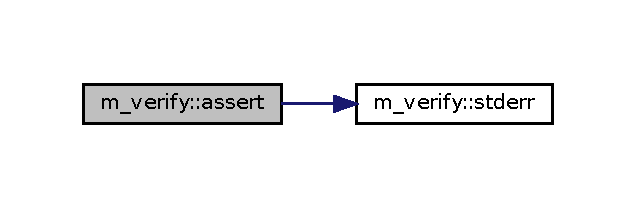
\includegraphics[width=305pt]{namespacem__verify_a83a6bafddb101d8b0fe70f34827836ff_cgraph}
\end{center}
\end{figure}
\mbox{\Hypertarget{namespacem__verify_a6185c00609b8f0e4c5a503cfadcb2490}\label{namespacem__verify_a6185c00609b8f0e4c5a503cfadcb2490}} 
\index{m\+\_\+verify@{m\+\_\+verify}!atleast@{atleast}}
\index{atleast@{atleast}!m\+\_\+verify@{m\+\_\+verify}}
\subsubsection{\texorpdfstring{atleast()}{atleast()}}
{\footnotesize\ttfamily function m\+\_\+verify\+::atleast (\begin{DoxyParamCaption}\item[{character(len=$\ast$), intent(in)}]{line,  }\item[{integer, intent(in)}]{length }\end{DoxyParamCaption})\hspace{0.3cm}{\ttfamily [private]}}

Here is the caller graph for this function\+:\nopagebreak
\begin{figure}[H]
\begin{center}
\leavevmode
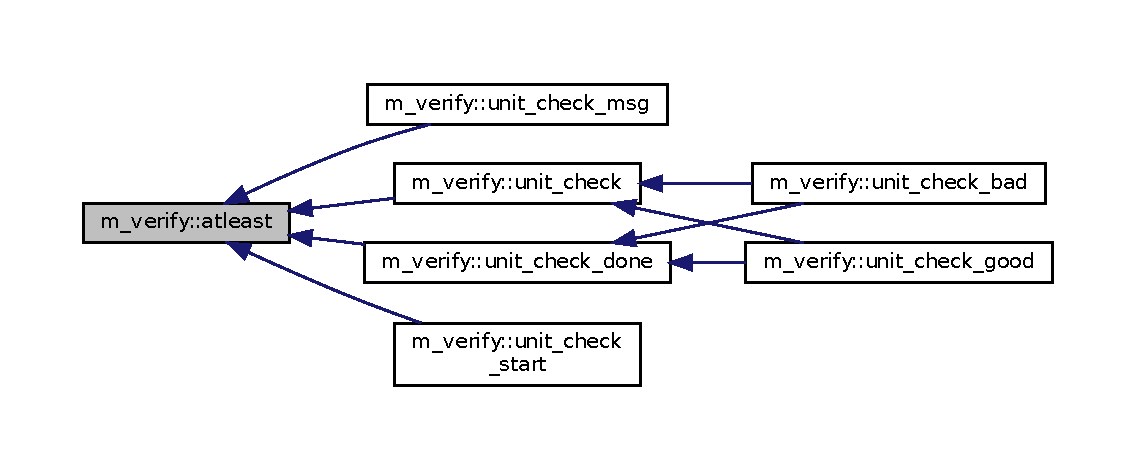
\includegraphics[width=350pt]{namespacem__verify_a6185c00609b8f0e4c5a503cfadcb2490_icgraph}
\end{center}
\end{figure}
\mbox{\Hypertarget{namespacem__verify_a7408df33e6934a8959fdeda8cc3fb5ff}\label{namespacem__verify_a7408df33e6934a8959fdeda8cc3fb5ff}} 
\index{m\+\_\+verify@{m\+\_\+verify}!dp\+\_\+accdig@{dp\+\_\+accdig}}
\index{dp\+\_\+accdig@{dp\+\_\+accdig}!m\+\_\+verify@{m\+\_\+verify}}
\subsubsection{\texorpdfstring{dp\+\_\+accdig()}{dp\_accdig()}}
{\footnotesize\ttfamily subroutine, public m\+\_\+verify\+::dp\+\_\+accdig (\begin{DoxyParamCaption}\item[{class($\ast$), intent(in)}]{x,  }\item[{class($\ast$), intent(in)}]{y,  }\item[{class($\ast$), intent(in)}]{digi0,  }\item[{real, intent(out)}]{A\+C\+U\+R\+CY,  }\item[{integer, intent(out)}]{I\+ND }\end{DoxyParamCaption})}



\subsubsection*{N\+A\+ME}

dp\+\_\+accdig(3f) -\/ \mbox{[}M\+\_\+verify\mbox{]} compare two numbers only up to a specified number of digits (L\+I\+C\+E\+N\+SE\+:PD) 

\subsubsection*{S\+Y\+N\+O\+P\+S\+IS}

\begin{DoxyVerb}   subroutine dp_accdig(x,y,digio,acurcy,ind)

    class(*),intent(in)  :: X
    class(*),intent(in)  :: Y
    class(*),intent(in)  :: DIGI0
    real,intent(out)     :: acurcy
    integer,intent(out)  :: ind
\end{DoxyVerb}


\subsubsection*{D\+E\+S\+C\+R\+I\+P\+T\+I\+ON}

\begin{DoxyVerb}This procedure is used to check how closely two numbers agree.

   call dp_accdig(X,Y,DIGI0,ACURCY,IND)

The values X and Y are the numbers to compare, and DIGI0 is the
threshold number of digits to consider significant in returning IND.

If X and Y are considered equal within DIGI0 relative tolerance,

    IND    = 0, if tolerance is     satisfied.
           = 1, if tolerance is not satisfied.

The result ACURCY gives a measure of the number of leading digits in X
which are the same as the number of leading digits in Y.

     ACURCY=-log10((X-Y)/Y)   if X != Y and Y != 0
     ACURCY=-log10(X-Y)       if X != Y and Y = 0
     ACURCY=8                 if X=Y

     ACURCY is never less than -8 or greater than 8 for REAL values

TOLERANCE ...
     X and Y are considered equal within DIGI0 relative tolerance,
     if ACURCY is greater than DIGI0.

For example, Take some numbers and compare then  to 1.2345678 ...

   ================================================
   A number     |    ACURCY       |   ACURCY
                |    1.2345678=Y  |   1.2345678=X
   ================================================
    1.234680    |    3.7900571    |   3.7901275
    1.2345378   |    4.6144510    |   4.6144404
    2.2234568   |    0.096367393  |   0.35188114
    1.2345678   |    8.0000000    |   8.0000000
    1.2345679   |    7.0732967    |   7.0731968
   -1.2345678   |   -0.30103000   |  -0.30103000
   76.234567    |   -1.7835463    |   0.0070906729
    2.4691356   |    0.0          |   0.3010300
    0.0         |    0.0          |  -0.91514942.

Due to the typical limits of the log function, the number of
significant digits in the result is best considered to be three.

Notice that 1.2345678=Y produces different values than 1.2345678=X

A negative result indicates the two values being compared either do
not agree in the first digit or they differ with respect to sign. An
example of two numbers which do not agree in their leading digit (and
actually differ in order of magnitude) is given above by X=76.234567
and Y=1.2345678; the accuracy reported is -1.7835463. An example of
two numbers which do not agree in sign in X=-1.2345678 and Y=1.2345678;
here the accuracy reported is -0.30103000.
\end{DoxyVerb}


\subsubsection*{E\+X\+A\+M\+P\+LE}

Example program\+:

program demo\+\_\+dp\+\_\+accdig ! fortran 90 example use M\+\_\+verify, only \+: dp\+\_\+accdig implicit none integer \+:\+: digi doubleprecision \+:\+: a, b integer \+:\+: i10, i20, i30 integer \+:\+: ind, ind1, ind2 real \+:\+: acurcy, acurcy1, acurcy2 doubleprecision \+:\+: vals(9) data vals/ \& \&1.\+234680d0, 1.\+2345378d0, 2.\+2234568d0, 1.\+2345678d0, \& \&1.\+2345679d0, -\/1.\+2345678d0, 76.\+234567d0, 2.\+4691356d0, \& \&0.\+0d0/ write($\ast$,$\ast$)\textquotesingle{}=========================\textquotesingle{} do i10=0,16 a=1.\+0d0 b=a+1.0d0/(10$\ast$$\ast$i10) call dp\+\_\+accdig(a,b,8.\+0,acurcy,ind) write($\ast$,$\ast$)i10,a,b,acurcy,ind enddo write($\ast$,$\ast$)\textquotesingle{}=========================\textquotesingle{} digi=16 do i20=0,digi a=1.\+0d0 b=a+1.0d0/(10$\ast$$\ast$i20) call dp\+\_\+accdig(a,b,dble(digi),acurcy,ind) write($\ast$,$\ast$)i20,a,b,acurcy,ind enddo write($\ast$,$\ast$)\textquotesingle{}=========================\textquotesingle{} do i30=1,9 call dp\+\_\+accdig(1.\+2345678d0,vals(i30),8.\+0,acurcy1,ind1) call dp\+\_\+accdig(vals(i30),1.\+2345678d0,8.\+0,acurcy2,ind2) write($\ast$,$\ast$)i30,vals(i30),acurcy1,acurcy2,ind1,ind2 enddo end program demo\+\_\+dp\+\_\+accdig

\subsubsection*{N\+O\+T\+ES}

\subsubsection*{R\+E\+F\+E\+R\+E\+N\+C\+ES}

based on ...

N\+BS O\+M\+N\+I\+T\+AB 1980 V\+E\+R\+S\+I\+ON 6.\+01 1/ 1/81. dp\+\_\+accdig V 7.\+00 2/14/90. $\ast$$\ast$ David Hogben, Statistical Engineering Division, Center for Computing and Applied Mathematics, A337 Administration Building, National Institute of Standards and Technology, Gaithersburg, MD 20899 T\+E\+L\+E\+P\+H\+O\+NE 301-\/975-\/2845 O\+R\+I\+G\+I\+N\+AL V\+E\+R\+S\+I\+ON -\/ October, 1969. C\+U\+R\+R\+E\+NT V\+E\+R\+S\+I\+ON -\/ February, 1990. J\+SU V\+E\+R\+S\+I\+ON -\/ February, 1991.

\subsubsection*{D\+E\+P\+E\+N\+D\+E\+N\+C\+I\+ES}

o M\+\_\+journal(), log10(), abs(1)

\subsubsection*{A\+U\+T\+H\+O\+RS}

David Hogben, John S. Urban

\subsubsection*{L\+I\+C\+E\+N\+SE}

Public Domain 

References anyscalar\+\_\+to\+\_\+real128().

Here is the call graph for this function\+:\nopagebreak
\begin{figure}[H]
\begin{center}
\leavevmode
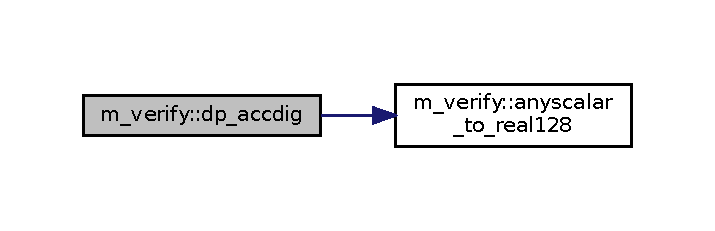
\includegraphics[width=343pt]{namespacem__verify_a7408df33e6934a8959fdeda8cc3fb5ff_cgraph}
\end{center}
\end{figure}
Here is the caller graph for this function\+:\nopagebreak
\begin{figure}[H]
\begin{center}
\leavevmode
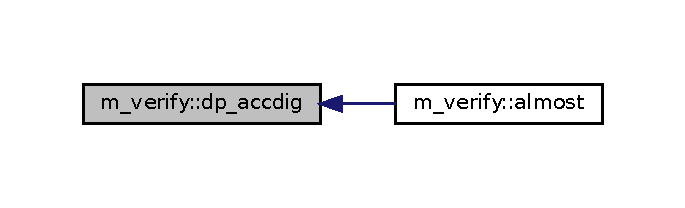
\includegraphics[width=329pt]{namespacem__verify_a7408df33e6934a8959fdeda8cc3fb5ff_icgraph}
\end{center}
\end{figure}
\mbox{\Hypertarget{namespacem__verify_a2695833d468118d68918d6aeabab6d0b}\label{namespacem__verify_a2695833d468118d68918d6aeabab6d0b}} 
\index{m\+\_\+verify@{m\+\_\+verify}!fstop@{fstop}}
\index{fstop@{fstop}!m\+\_\+verify@{m\+\_\+verify}}
\subsubsection{\texorpdfstring{fstop()}{fstop()}}
{\footnotesize\ttfamily subroutine, public m\+\_\+verify\+::fstop (\begin{DoxyParamCaption}\item[{integer, intent(in)}]{ierr,  }\item[{character(len=$\ast$), intent(in), optional}]{stdout,  }\item[{character(len=$\ast$), intent(in), optional}]{stderr }\end{DoxyParamCaption})}



\subsubsection*{N\+A\+ME}

fstop(3f) -\/ \mbox{[}M\+\_\+verify\mbox{]} call stop with both a number and a message (L\+I\+C\+E\+N\+SE\+:PD) \subsubsection*{S\+Y\+N\+O\+P\+S\+IS}

subroutine fstop(ierr,stdout,stderr)

integer,intent(in) \+:\+: ierr character(len=$\ast$),intent(in),optional \+:\+: stdout character(len=$\ast$),intent(in),optional \+:\+: stderr \subsubsection*{D\+E\+S\+C\+R\+I\+P\+T\+I\+ON}

F\+S\+T\+O\+P(3f) call S\+T\+O\+P(3f). What a call to S\+T\+OP does is very system dependent, so using an abstraction layer is useful, as it allows just the \mbox{\hyperlink{namespacem__verify_a2695833d468118d68918d6aeabab6d0b}{fstop()}} routine to be changed; and S\+T\+OP does not allow a variable to be used on the numeric access status (this has changed at f2015).

\subsubsection*{O\+P\+T\+I\+O\+NS}

ierr -\/ value in range 0 to 32 stdout -\/ description to be printed to standard output stderr -\/ description to be printed to standard error \subsubsection*{E\+X\+A\+M\+P\+L\+ES}

Sample program\+:

program demo\+\_\+fstop use M\+\_\+verify, only\+: fstop implicit none integer \+:\+: int write($\ast$,$\ast$)\textquotesingle{}Enter stop value\textquotesingle{} read($\ast$,$\ast$) int select case(int) case(10) ; call fstop(int) case(20) ; call fstop(int,stderr=\textquotesingle{}error\+: program will now stop\textquotesingle{}) case(25) ; call fstop(int,stdout=\textquotesingle{}stdout message\textquotesingle{},stderr=\textquotesingle{}stderr message\textquotesingle{}) case(30) ; call fstop(int,stdout=\textquotesingle{}error\+: program will now stop\textquotesingle{}) case default call fstop(int) endselect

end program demo\+\_\+fstop

Results\+:

\subsubsection*{S\+EE A\+L\+SO}

Look for common extensions, such as abort(3f), backtrace(3f)

\subsubsection*{A\+U\+T\+H\+OR}

John S. Urban \subsubsection*{L\+I\+C\+E\+N\+SE}

Public Domain 

References stderr().

Here is the call graph for this function\+:\nopagebreak
\begin{figure}[H]
\begin{center}
\leavevmode
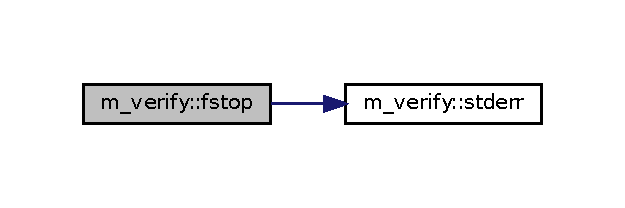
\includegraphics[width=300pt]{namespacem__verify_a2695833d468118d68918d6aeabab6d0b_cgraph}
\end{center}
\end{figure}
Here is the caller graph for this function\+:\nopagebreak
\begin{figure}[H]
\begin{center}
\leavevmode
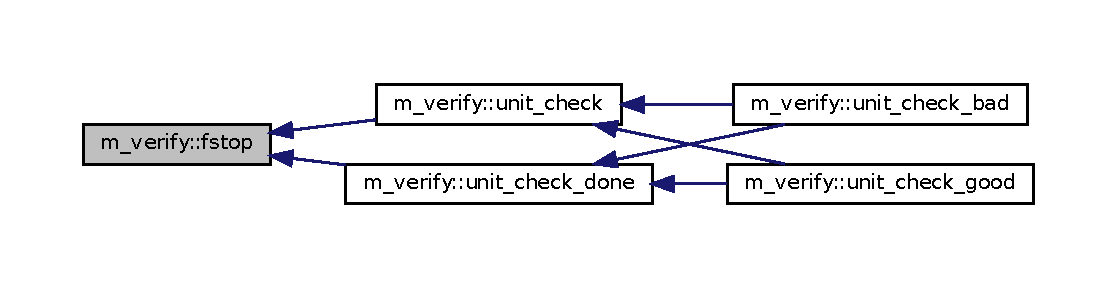
\includegraphics[width=350pt]{namespacem__verify_a2695833d468118d68918d6aeabab6d0b_icgraph}
\end{center}
\end{figure}
\mbox{\Hypertarget{namespacem__verify_aa0d8de1c26ca3aae0366b9fb8ead21c4}\label{namespacem__verify_aa0d8de1c26ca3aae0366b9fb8ead21c4}} 
\index{m\+\_\+verify@{m\+\_\+verify}!in\+\_\+margin@{in\+\_\+margin}}
\index{in\+\_\+margin@{in\+\_\+margin}!m\+\_\+verify@{m\+\_\+verify}}
\subsubsection{\texorpdfstring{in\+\_\+margin()}{in\_margin()}}
{\footnotesize\ttfamily elemental pure logical function, public m\+\_\+verify\+::in\+\_\+margin (\begin{DoxyParamCaption}\item[{class($\ast$), intent(in)}]{expected\+\_\+value,  }\item[{class($\ast$), intent(in)}]{measured\+\_\+value,  }\item[{class($\ast$), intent(in)}]{allowed\+\_\+margin }\end{DoxyParamCaption})}



\subsubsection*{N\+A\+ME}

in\+\_\+margin(3f) -\/ \mbox{[}M\+\_\+verify\mbox{]} check if two reals are approximately equal using a relative margin 

\subsubsection*{S\+Y\+N\+O\+P\+S\+IS}

\begin{DoxyVerb} elemental pure function in_margin( expected_value, measured_value, allowed_margin )

  real, intent(in)    :: expected_value
  real, intent(in)    :: measured_value
  real, intent(in)    :: allowed_margin
  class(*),intent(in) :: invalue
\end{DoxyVerb}


\subsubsection*{D\+E\+S\+C\+R\+I\+P\+T\+I\+ON}

Compare two values to see if they are relatively equal using the specified allowed margin. That is, see if V\+A\+L\+U\+E\+\_\+\+M\+E\+A\+S\+U\+R\+ED is in the range V\+A\+L\+U\+E\+\_\+\+E\+X\+P\+E\+C\+T\+ED +-\/ A\+L\+L\+O\+W\+E\+D\+\_\+\+E\+R\+R\+OR where the allowed error varies with the magnitude of the values, such that the allowed error is margin $\ast$ average magnitude of measured and expected).

So the allowed error is smaller when the magnitudes are smaller.

\subsubsection*{O\+P\+T\+I\+O\+NS}

expected\+\_\+value First value measured\+\_\+value Second value allowed\+\_\+margin Allowed relative margin

\subsubsection*{E\+X\+A\+M\+P\+LE}

Sample program\+:

program demo\+\_\+in\+\_\+margin use \+:\+: M\+\_\+verify, only \+: in\+\_\+margin implicit none write($\ast$,$\ast$) in\+\_\+margin(4.\+00000,3.\+99999,0.\+000000001) write($\ast$,$\ast$) in\+\_\+margin(4.\+00000,3.\+99999,0.\+00000001) write($\ast$,$\ast$) in\+\_\+margin(4.\+00000,3.\+99999,0.\+0000001) write($\ast$,$\ast$) in\+\_\+margin(4.\+00000,3.\+99999,0.\+000001)

write($\ast$,$\ast$) in\+\_\+margin(\mbox{[}4.\+0,40.\+0,400.\+0,4000.\+0,40000.\+0\mbox{]}, \mbox{[}3.\+9,39.\+9,399.\+9,3999.\+9,39999.\+9\mbox{]} ,0.\+000001) write($\ast$,$\ast$) in\+\_\+margin(\mbox{[}4.\+0,40.\+0,400.\+0,4000.\+0,40000.\+0\mbox{]}, \mbox{[}3.\+9,39.\+9,399.\+9,3999.\+9,39999.\+9\mbox{]} ,0.\+00001)

write($\ast$,$\ast$) in\+\_\+margin(4.\+00000,3.\+99999,0.\+00001) write($\ast$,$\ast$) in\+\_\+margin(4.\+00000,3.\+99999,0.\+0001) write($\ast$,$\ast$) in\+\_\+margin(4.\+00000,3.\+99999,0.\+001) write($\ast$,$\ast$) in\+\_\+margin(4.\+00000,3.\+99999,0.\+01)

end program demo\+\_\+in\+\_\+margin

Results\+:

F F F F F F F F F F F F F T T T T T 

References anyscalar\+\_\+to\+\_\+double().

Here is the call graph for this function\+:\nopagebreak
\begin{figure}[H]
\begin{center}
\leavevmode
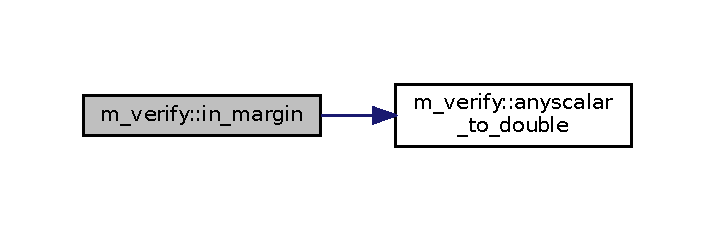
\includegraphics[width=343pt]{namespacem__verify_aa0d8de1c26ca3aae0366b9fb8ead21c4_cgraph}
\end{center}
\end{figure}
\mbox{\Hypertarget{namespacem__verify_a1a97667eb1d53ce5b97a60c4a9ebe565}\label{namespacem__verify_a1a97667eb1d53ce5b97a60c4a9ebe565}} 
\index{m\+\_\+verify@{m\+\_\+verify}!julian@{julian}}
\index{julian@{julian}!m\+\_\+verify@{m\+\_\+verify}}
\subsubsection{\texorpdfstring{julian()}{julian()}}
{\footnotesize\ttfamily real(kind=\mbox{\hyperlink{namespacem__verify_a7f6aa94b09b3824bc5c15bc74e757d6b}{realtime}}) function m\+\_\+verify\+::julian (\begin{DoxyParamCaption}{ }\end{DoxyParamCaption})\hspace{0.3cm}{\ttfamily [private]}}

Here is the caller graph for this function\+:\nopagebreak
\begin{figure}[H]
\begin{center}
\leavevmode
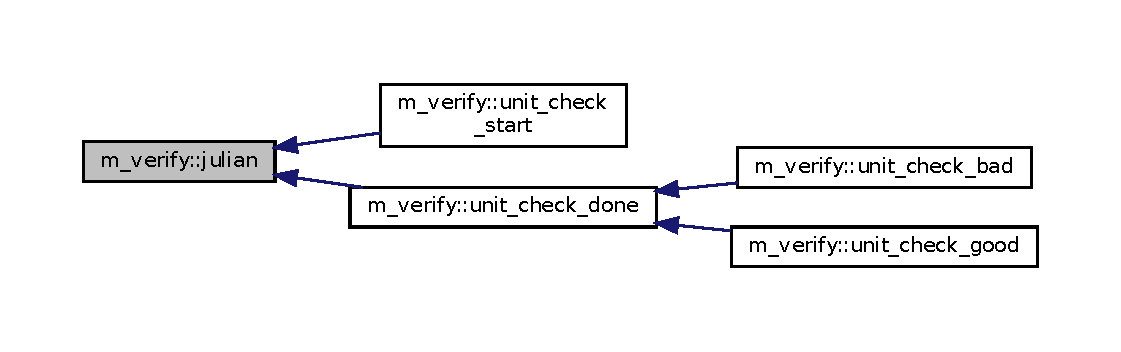
\includegraphics[width=350pt]{namespacem__verify_a1a97667eb1d53ce5b97a60c4a9ebe565_icgraph}
\end{center}
\end{figure}
\mbox{\Hypertarget{namespacem__verify_aa772ce395fd2e4cc546b8645d8fd9949}\label{namespacem__verify_aa772ce395fd2e4cc546b8645d8fd9949}} 
\index{m\+\_\+verify@{m\+\_\+verify}!pdec@{pdec}}
\index{pdec@{pdec}!m\+\_\+verify@{m\+\_\+verify}}
\subsubsection{\texorpdfstring{pdec()}{pdec()}}
{\footnotesize\ttfamily subroutine, public m\+\_\+verify\+::pdec (\begin{DoxyParamCaption}\item[{character(len=$\ast$), intent(in)}]{string }\end{DoxyParamCaption})}



\subsubsection*{N\+A\+ME}

pdec(3f) -\/ \mbox{[}M\+\_\+verify\mbox{]} write out string with A\+S\+C\+II decimal equivalent vertically under it (L\+I\+C\+E\+N\+SE\+:PD) 

\subsubsection*{S\+Y\+N\+O\+P\+S\+IS}

\begin{DoxyVerb}Usage:

 subroutine pdec(string)
 character(len=*),intent(in) :: string
\end{DoxyVerb}


\subsubsection*{D\+E\+S\+C\+R\+I\+P\+T\+I\+ON}

\begin{DoxyVerb}Given a string to print, PDEC() writes out the ASCII Decimal equivalent
of the string directly underneath it. This can help you to locate
unprintable characters or non-standard white-space such as a backspace
character or tab character in input strings that your program could
not interpret. On output, non-printable characters are replaced with
a space, and trailing spaces are ignored.

You read the numbers vertically.

1. ignore trailing spaces
2. print the character if it has an ADE of 32 on up
3. print a space if it has an ADE of less than 32
4. underneath each character print the ADE value vertically
5. strings are assumed under 32767 characters in length.
   Format integer constants > 32767 are not supported on HP-UX
   when newer compilers are available use unlimited
\end{DoxyVerb}


\subsubsection*{E\+X\+A\+M\+P\+L\+ES}

\begin{DoxyVerb}Sample program:

   program demo_pdec
   use M_verify, only : pdec
   call pdec(' ABCDEFG abcdefg    ')
   end program demo_pdec

would produce (notice trailing space is trimmed):

  > ABCDEFG abcdefg
  >0000000000001111
  >3666667739990000
  >2567890127890123
\end{DoxyVerb}


\subsubsection*{A\+U\+T\+H\+OR}

John S. Urban \subsubsection*{L\+I\+C\+E\+N\+SE}

Public Domain \mbox{\Hypertarget{namespacem__verify_af997c802e1ad966d55f023822b2f645a}\label{namespacem__verify_af997c802e1ad966d55f023822b2f645a}} 
\index{m\+\_\+verify@{m\+\_\+verify}!round@{round}}
\index{round@{round}!m\+\_\+verify@{m\+\_\+verify}}
\subsubsection{\texorpdfstring{round()}{round()}}
{\footnotesize\ttfamily real(kind=dp) function, public m\+\_\+verify\+::round (\begin{DoxyParamCaption}\item[{real(kind=dp), intent(in)}]{val,  }\item[{integer, intent(in)}]{idigits0 }\end{DoxyParamCaption})}

\mbox{\Hypertarget{namespacem__verify_a41f795f932767c97b5ef481a694f4f84}\label{namespacem__verify_a41f795f932767c97b5ef481a694f4f84}} 
\index{m\+\_\+verify@{m\+\_\+verify}!stderr@{stderr}}
\index{stderr@{stderr}!m\+\_\+verify@{m\+\_\+verify}}
\subsubsection{\texorpdfstring{stderr()}{stderr()}}
{\footnotesize\ttfamily subroutine, public m\+\_\+verify\+::stderr (\begin{DoxyParamCaption}\item[{class($\ast$), intent(in), optional}]{msg,  }\item[{class($\ast$), intent(in), optional}]{gen0,  }\item[{class($\ast$), intent(in), optional}]{gen1,  }\item[{class($\ast$), intent(in), optional}]{gen2,  }\item[{class($\ast$), intent(in), optional}]{gen3,  }\item[{class($\ast$), intent(in), optional}]{gen4,  }\item[{class($\ast$), intent(in), optional}]{gen5,  }\item[{class($\ast$), intent(in), optional}]{gen6,  }\item[{class($\ast$), intent(in), optional}]{gen7,  }\item[{class($\ast$), intent(in), optional}]{gen8,  }\item[{class($\ast$), intent(in), optional}]{gen9 }\end{DoxyParamCaption})}



\subsubsection*{N\+A\+ME}

stderr(3f) -\/ \mbox{[}M\+\_\+verify\mbox{]} write message to stderr (L\+I\+C\+E\+N\+SE\+:PD) \subsubsection*{S\+Y\+N\+O\+P\+S\+IS}

subroutine stderr(msg,\mbox{[}generic\mbox{]})

class($\ast$),intent(in),optional \+:\+: msg class($\ast$),intent(in),optional \+:\+: generic0,generic1,generic2,generic3,generic4 class($\ast$),intent(in),optional \+:\+: generic5,generic6,generic7,generic8,generic9 \subsubsection*{D\+E\+S\+C\+R\+I\+P\+T\+I\+ON}

S\+T\+D\+E\+R\+R(3f) writes a message to standard error using a standard f2003 method. Up to ten generic options are available. \subsubsection*{O\+P\+T\+I\+O\+NS}

msg -\/ description to print generic\mbox{[}0-\/9\mbox{]} -\/ optional value to print the value of after the message. May be of type I\+N\+T\+E\+G\+ER, L\+O\+G\+I\+C\+AL, R\+E\+AL, D\+O\+U\+B\+L\+E\+P\+R\+E\+C\+I\+S\+I\+ON, C\+O\+M\+P\+L\+EX, or C\+H\+A\+R\+A\+C\+T\+ER. \subsubsection*{E\+X\+A\+M\+P\+L\+ES}

Sample program\+:

program demo\+\_\+stderr use,intrinsic \+:\+: iso\+\_\+fortran\+\_\+env, only \+: int8, int16, int32, int64 use,intrinsic \+:\+: iso\+\_\+fortran\+\_\+env, only \+: real32, real64, real128 use,intrinsic \+:\+: iso\+\_\+fortran\+\_\+env, only \+: real=$>$ real32, integer=$>$ int32 use M\+\_\+verify, only\+: stderr implicit none

call stderr(\textquotesingle{}A simple message\textquotesingle{}) call stderr(\textquotesingle{}error\+: R\+V\+A\+L\+UE=\textquotesingle{},3.\+0/4.0) call stderr(\textquotesingle{}error\+: I\+V\+A\+L\+UE=\textquotesingle{},123456789) call stderr(\textquotesingle{}error\+: L\+V\+A\+L\+UE=\textquotesingle{},.true.)

S\+E\+V\+E\+R\+AL\+: block integer \+:\+: least=10, most=999, ival=-\/10 call stderr(\textquotesingle{}error\+: value\textquotesingle{},ival,\textquotesingle{}should be between\textquotesingle{},least,\textquotesingle{}and\textquotesingle{},most) endblock S\+E\+V\+E\+R\+AL

call stderr(\textquotesingle{}real32 \+:\textquotesingle{},huge(0.\+0\+\_\+real32),0.\+0\+\_\+real32,12345.\+6789\+\_\+real32,tiny(0.\+0\+\_\+real32)) call stderr(\textquotesingle{}real64 \+:\textquotesingle{},huge(0.\+0\+\_\+real64),0.\+0\+\_\+real64,12345.\+6789\+\_\+real64,tiny(0.\+0\+\_\+real64)) call stderr(\textquotesingle{}real128 \+:\textquotesingle{},huge(0.\+0\+\_\+real128),0.\+0\+\_\+real128,12345.\+6789\+\_\+real128,tiny(0.\+0\+\_\+real128)) call stderr(\textquotesingle{}complex \+:\textquotesingle{},cmplx(huge(0.\+0\+\_\+real),tiny(0.\+0\+\_\+real)))

call stderr(\textquotesingle{}error\+: program will now stop\textquotesingle{}) stop 1

end program demo\+\_\+stderr

Results\+: A simple message error\+: R\+V\+A\+L\+UE= 0.\+750000000 error\+: I\+V\+A\+L\+UE= 123456789 error\+: L\+V\+A\+L\+UE= T error\+: value -\/10 should be between 10 and 999 real32 \+: 3.\+40282347E+38 ... 0.\+00000000 ... 12345.\+6787 ... 1.\+17549435E-\/38 real64 \+: 1.\+7976931348623157E+308 ... 0.\+0000000000000000 ... 12345.\+678900000001 ... 2.\+2250738585072014E-\/308 real128 \+: 1.\+18973149535723176508575932662800702E+4932 ... 0.\+00000000000000000000000000000000000 ... 12345.\+6789000000000000000000000000002 ... 3.\+36210314311209350626267781732175260E-\/4932 complex \+: (3.\+40282347E+38,1.\+17549435E-\/38) error\+: program will now stop \subsection*{S\+T\+OP 1 }

\subsubsection*{A\+U\+T\+H\+OR}

John S. Urban \subsubsection*{L\+I\+C\+E\+N\+SE}

Public Domain Here is the caller graph for this function\+:\nopagebreak
\begin{figure}[H]
\begin{center}
\leavevmode
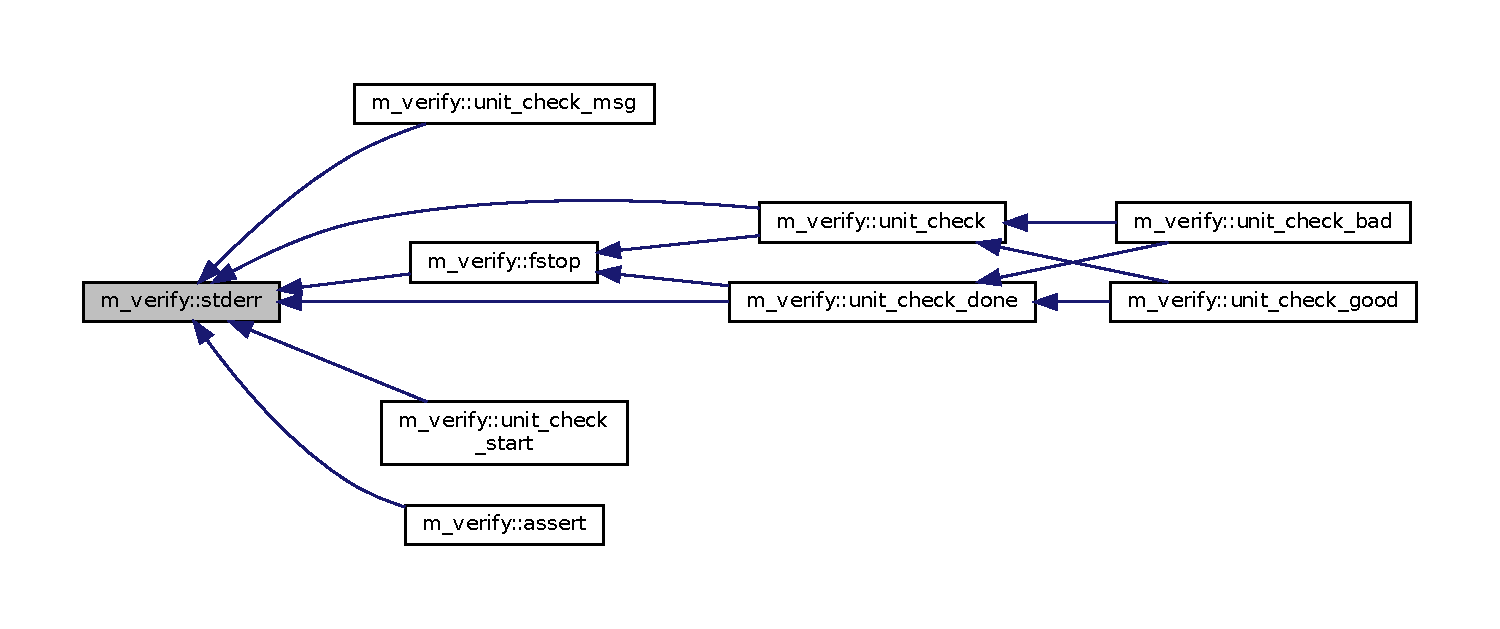
\includegraphics[width=350pt]{namespacem__verify_a41f795f932767c97b5ef481a694f4f84_icgraph}
\end{center}
\end{figure}
\mbox{\Hypertarget{namespacem__verify_a96149da1a302f2a157d79dadc94e755e}\label{namespacem__verify_a96149da1a302f2a157d79dadc94e755e}} 
\index{m\+\_\+verify@{m\+\_\+verify}!unit\+\_\+check@{unit\+\_\+check}}
\index{unit\+\_\+check@{unit\+\_\+check}!m\+\_\+verify@{m\+\_\+verify}}
\subsubsection{\texorpdfstring{unit\+\_\+check()}{unit\_check()}}
{\footnotesize\ttfamily subroutine, public m\+\_\+verify\+::unit\+\_\+check (\begin{DoxyParamCaption}\item[{character(len=$\ast$), intent(in)}]{name,  }\item[{logical, intent(in)}]{logical\+\_\+expression,  }\item[{class($\ast$), intent(in), optional}]{msg,  }\item[{class($\ast$), intent(in), optional}]{msg1,  }\item[{class($\ast$), intent(in), optional}]{msg2,  }\item[{class($\ast$), intent(in), optional}]{msg3,  }\item[{class($\ast$), intent(in), optional}]{msg4,  }\item[{class($\ast$), intent(in), optional}]{msg5,  }\item[{class($\ast$), intent(in), optional}]{msg6,  }\item[{class($\ast$), intent(in), optional}]{msg7,  }\item[{class($\ast$), intent(in), optional}]{msg8,  }\item[{class($\ast$), intent(in), optional}]{msg9 }\end{DoxyParamCaption})}



\subsubsection*{N\+A\+ME}

unit\+\_\+check(3f) -\/ \mbox{[}M\+\_\+verify\mbox{]} if logical expression is false, call command \char`\"{}goodbad N\+A\+M\+E bad\char`\"{} and stop program by default (L\+I\+C\+E\+N\+SE\+:PD) 

\subsubsection*{S\+Y\+N\+O\+P\+S\+IS}

\begin{DoxyVerb}subroutine unit_check(name,expression,msg,msg1,msg2,msg3,msg4,msg5,msg6,msg7,msg8,msg9)

 character(len=*),intent(in) :: name
 logical,intent(in) :: expression
 class(*),intent(in),optional :: msg,msg1,msg2,msg3,msg4,msg5,msg6,msg7,msg8,msg9
\end{DoxyVerb}


\subsubsection*{D\+E\+S\+C\+R\+I\+P\+T\+I\+ON}

unit\+\_\+check(3f) tests the expression and if it is false, calls the shell command \begin{DoxyVerb} goodbad NAME bad
\end{DoxyVerb}


and stops the program. \subsubsection*{O\+P\+T\+I\+O\+NS}

N\+A\+ME the unit test name passed on to the goodbad(1) command E\+X\+P\+R\+E\+S\+S\+I\+ON the logical expression to evaluate M\+SG,M\+S\+G1...M\+S\+G9 optional message to display when performing test, composed of any scalar intrinsics of type I\+N\+T\+E\+G\+ER, R\+E\+AL, D\+O\+U\+B\+L\+E\+P\+R\+E\+C\+I\+S\+I\+ON, C\+O\+M\+P\+L\+EX, L\+O\+G\+I\+C\+AL, or C\+H\+A\+R\+A\+C\+T\+ER, with a space placed between each value.

\subsubsection*{E\+X\+A\+M\+P\+L\+ES}

Sample program\+:

program demo\+\_\+unit\+\_\+check use M\+\_\+verify, only\+: unit\+\_\+check use M\+\_\+verify, only\+: unit\+\_\+check\+\_\+start use M\+\_\+verify, only\+: unit\+\_\+check\+\_\+done use M\+\_\+verify, only\+: almost

!!use M\+\_\+verify, only\+: unit\+\_\+check\+\_\+keep\+\_\+going ! default is unit\+\_\+check\+\_\+keep\+\_\+going=.false. !!use M\+\_\+verify, only\+: debug ! default is .false. !!use M\+\_\+verify, only\+: unit\+\_\+check\+\_\+command ! default is unit\+\_\+check\+\_\+command=\textquotesingle{}goodbad\textquotesingle{}

implicit none integer \+:\+: i integer \+:\+: x integer,allocatable \+:\+: arr(\+:) real,allocatable \+:\+: arr1(\+:) real,allocatable \+:\+: arr2(\+:)

!!unit\+\_\+check\+\_\+command=\textquotesingle{}\textquotesingle{} x=10 arr1=\mbox{[}1.\+0,10.\+0,100.\+0\mbox{]} arr2=\mbox{[}1.\+0001,10.\+001,100.\+01\mbox{]} call unit\+\_\+check\+\_\+start(\textquotesingle{}myroutine\textquotesingle{})

call unit\+\_\+check(\textquotesingle{}myroutine\textquotesingle{}, x.\+gt.\+3 ,\textquotesingle{}test if big enough\textquotesingle{}) call unit\+\_\+check(\textquotesingle{}myroutine\textquotesingle{}, x.\+lt.\+100 ,\textquotesingle{}test if small enough\textquotesingle{})

do i=1,size(arr1) call unit\+\_\+check(\textquotesingle{}myroutine\textquotesingle{}, almost(arr1(i),arr2(i),3.\+9,verbose=.true.) ) enddo

arr=\mbox{[}10,20,30\mbox{]} call unit\+\_\+check(\textquotesingle{}myroutine\textquotesingle{}, .not.\+any(arr.\+lt.\+0) ,\textquotesingle{}test if any negative values in array A\+RR\textquotesingle{}) call unit\+\_\+check(\textquotesingle{}myroutine\textquotesingle{}, all(arr.\+lt.\+100) ,\textquotesingle{}test if all values less than 100 in array A\+RR\textquotesingle{})

call unit\+\_\+check\+\_\+done(\textquotesingle{}myroutine\textquotesingle{},msg=\textquotesingle{}checks on \char`\"{}myroutine\char`\"{} all passed\textquotesingle{})

end program demo\+\_\+unit\+\_\+check

Sample output (varies with what goodbad(1) command is used)\+:

unit\+\_\+check\+: myroutine S\+U\+C\+C\+E\+SS\+:test if big enough unit\+\_\+check\+: myroutine S\+U\+C\+C\+E\+SS\+:test if small enough unit\+\_\+check\+: myroutine S\+U\+C\+C\+E\+SS\+:test if any negative values in array A\+RR unit\+\_\+check\+: myroutine S\+U\+C\+C\+E\+SS\+:test if all values less than 100 in array A\+RR {\itshape almost} for values 1.\+00000000 1.\+00010002 agreement of 3.\+99997139 digits out of requested 3.\+90000010 {\itshape almost} for values 10.\+0000000 10.\+0010004 agreement of 3.\+99986792 digits out of requested 3.\+90000010 {\itshape almost} for values 100.\+000000 100.\+010002 agreement of 3.\+99995065 digits out of requested 3.\+90000010 unit\+\_\+check\+\_\+good\+: myroutine P\+A\+S\+S\+ED\+:checks on \char`\"{}myroutine\char`\"{} all passed

\subsubsection*{A\+U\+T\+H\+OR}

John S. Urban \subsubsection*{L\+I\+C\+E\+N\+SE}

Public Domain 

References atleast(), fstop(), ifailed\+\_\+g, ipassed\+\_\+g, no\+\_\+news\+\_\+is\+\_\+good\+\_\+news, stderr(), unit\+\_\+check\+\_\+command, and unit\+\_\+check\+\_\+keep\+\_\+going.

Here is the call graph for this function\+:\nopagebreak
\begin{figure}[H]
\begin{center}
\leavevmode
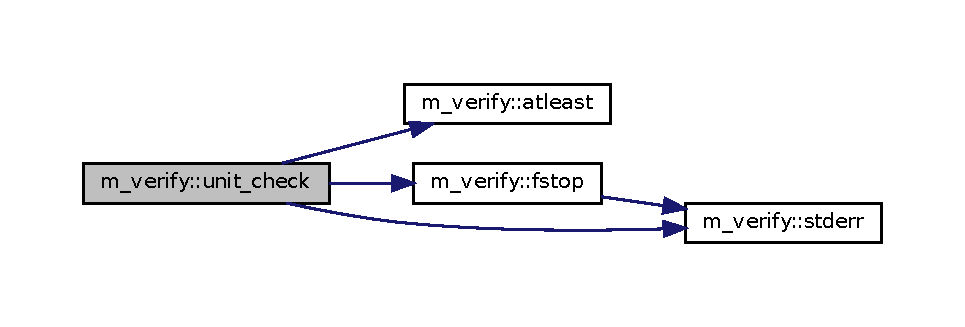
\includegraphics[width=350pt]{namespacem__verify_a96149da1a302f2a157d79dadc94e755e_cgraph}
\end{center}
\end{figure}
Here is the caller graph for this function\+:\nopagebreak
\begin{figure}[H]
\begin{center}
\leavevmode
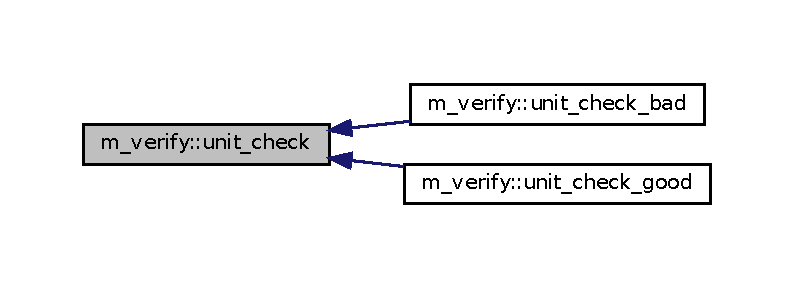
\includegraphics[width=350pt]{namespacem__verify_a96149da1a302f2a157d79dadc94e755e_icgraph}
\end{center}
\end{figure}
\mbox{\Hypertarget{namespacem__verify_aaa2744e5ab1687072183869bd53cc086}\label{namespacem__verify_aaa2744e5ab1687072183869bd53cc086}} 
\index{m\+\_\+verify@{m\+\_\+verify}!unit\+\_\+check\+\_\+bad@{unit\+\_\+check\+\_\+bad}}
\index{unit\+\_\+check\+\_\+bad@{unit\+\_\+check\+\_\+bad}!m\+\_\+verify@{m\+\_\+verify}}
\subsubsection{\texorpdfstring{unit\+\_\+check\+\_\+bad()}{unit\_check\_bad()}}
{\footnotesize\ttfamily subroutine, public m\+\_\+verify\+::unit\+\_\+check\+\_\+bad (\begin{DoxyParamCaption}\item[{character(len=$\ast$), intent(in)}]{name,  }\item[{character(len=$\ast$), intent(in), optional}]{opts,  }\item[{character(len=$\ast$), intent(in), optional}]{msg }\end{DoxyParamCaption})}



\subsubsection*{N\+A\+ME}

unit\+\_\+check\+\_\+bad(3f) -\/ \mbox{[}M\+\_\+verify\mbox{]} call command \char`\"{}goodbad N\+A\+M\+E bad\char`\"{} and stop program (L\+I\+C\+E\+N\+SE\+:PD) 

\subsubsection*{S\+Y\+N\+O\+P\+S\+IS}

\begin{DoxyVerb}subroutine unit_check_bad(name,opts,msg)

 character(len=*),intent(in) :: name
 character(len=*),intent(in),optional :: opts
 character(len=*),intent(in),optional :: msg
\end{DoxyVerb}


\subsubsection*{D\+E\+S\+C\+R\+I\+P\+T\+I\+ON}

\begin{DoxyVerb}unit_check_bad(3f) calls the shell command

     goodbad NAME bad [opts]

and stops the program. It is just a shortcut for calling
     call unit_check(name,.false.)
     call unit_check_done(name,opts,msg)
\end{DoxyVerb}


\subsubsection*{E\+X\+A\+M\+P\+L\+ES}

Sample program\+:

program demo\+\_\+unit\+\_\+check\+\_\+bad use M\+\_\+verify, only\+: unit\+\_\+check\+\_\+start use M\+\_\+verify, only\+: unit\+\_\+check use M\+\_\+verify, only\+: unit\+\_\+check\+\_\+good, unit\+\_\+check\+\_\+bad

implicit none integer \+:\+: x x=10 call unit\+\_\+check\+\_\+start(\textquotesingle{}myroutine\textquotesingle{})

call unit\+\_\+check(\textquotesingle{}myroutine\textquotesingle{}, x.\+gt.\+3 ,\textquotesingle{}test if big enough\textquotesingle{}) call unit\+\_\+check(\textquotesingle{}myroutine\textquotesingle{}, x.\+lt.\+100 ,\textquotesingle{}test if small enough\textquotesingle{})

if(x.\+ne.\+0)then call unit\+\_\+check\+\_\+bad (\textquotesingle{}myroutine\textquotesingle{},msg=\textquotesingle{}checks on \char`\"{}myroutine\char`\"{} failed\textquotesingle{}) ! program execution stopped endif

end program demo\+\_\+unit\+\_\+check\+\_\+bad

\subsubsection*{A\+U\+T\+H\+OR}

John S. Urban

\subsubsection*{L\+I\+C\+E\+N\+SE}

Public Domain 

References unit\+\_\+check(), and unit\+\_\+check\+\_\+done().

Here is the call graph for this function\+:\nopagebreak
\begin{figure}[H]
\begin{center}
\leavevmode
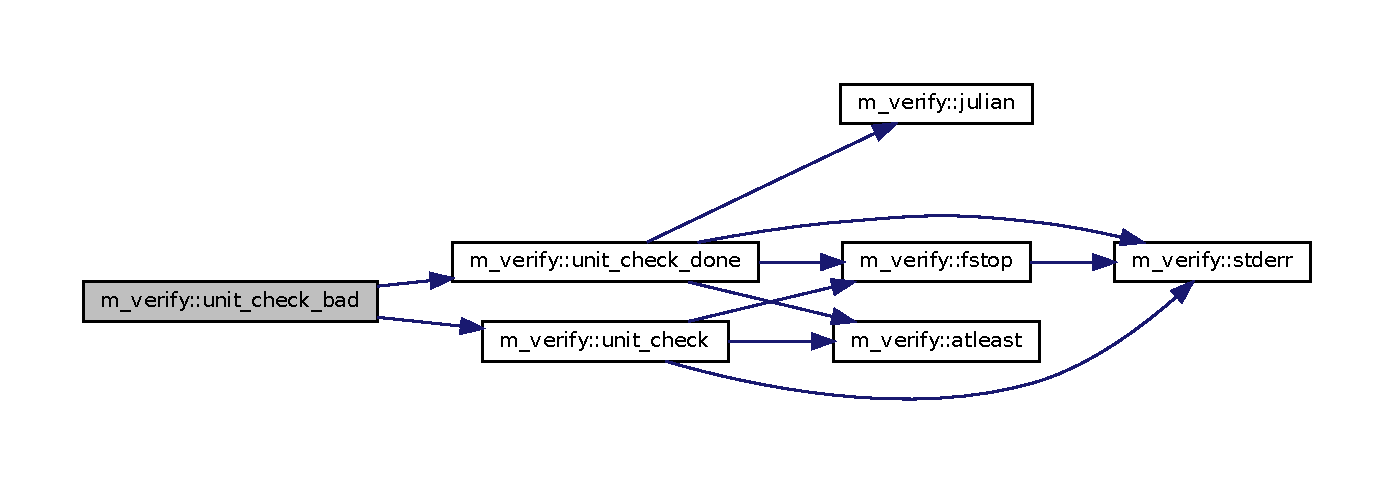
\includegraphics[width=350pt]{namespacem__verify_aaa2744e5ab1687072183869bd53cc086_cgraph}
\end{center}
\end{figure}
\mbox{\Hypertarget{namespacem__verify_a0c0ed723b61b2cbbebb81fa91edd1941}\label{namespacem__verify_a0c0ed723b61b2cbbebb81fa91edd1941}} 
\index{m\+\_\+verify@{m\+\_\+verify}!unit\+\_\+check\+\_\+done@{unit\+\_\+check\+\_\+done}}
\index{unit\+\_\+check\+\_\+done@{unit\+\_\+check\+\_\+done}!m\+\_\+verify@{m\+\_\+verify}}
\subsubsection{\texorpdfstring{unit\+\_\+check\+\_\+done()}{unit\_check\_done()}}
{\footnotesize\ttfamily subroutine, public m\+\_\+verify\+::unit\+\_\+check\+\_\+done (\begin{DoxyParamCaption}\item[{character(len=$\ast$), intent(in)}]{name,  }\item[{character(len=$\ast$), intent(in), optional}]{opts,  }\item[{character(len=$\ast$), intent(in), optional}]{msg }\end{DoxyParamCaption})}



\subsubsection*{N\+A\+ME}

unit\+\_\+check\+\_\+done(3f) -\/ \mbox{[}M\+\_\+verify\mbox{]} call command \char`\"{}goodbad N\+A\+M\+E good\char`\"{} or \char`\"{}goodbad N\+A\+M\+E bad\char`\"{} depending on whether failures were found (L\+I\+C\+E\+N\+SE\+:PD) 

\subsubsection*{S\+Y\+N\+O\+P\+S\+IS}

\begin{DoxyVerb}subroutine unit_check_done(name,opts,msg)

 character(len=*),intent(in) :: name
 character(len=*),intent(in),optional :: opts
 character(len=*),intent(in),optional :: msg
\end{DoxyVerb}


\subsubsection*{D\+E\+S\+C\+R\+I\+P\+T\+I\+ON}

\begin{DoxyVerb}If there have been no failures the shell command

     goodbad NAME good [opts]

is executed, else the command

     goodbad NAME bad [opts]

is executed and by default stops the program if their have been
any failures.
\end{DoxyVerb}


\subsubsection*{E\+X\+A\+M\+P\+L\+ES}

Sample program\+:

program demo\+\_\+unit\+\_\+check\+\_\+done use M\+\_\+verify, only\+: unit\+\_\+check\+\_\+start use M\+\_\+verify, only\+: unit\+\_\+check use M\+\_\+verify, only\+: unit\+\_\+check\+\_\+good, unit\+\_\+check\+\_\+done, unit\+\_\+check\+\_\+bad

implicit none integer \+:\+: x x=10 call unit\+\_\+check\+\_\+start(\textquotesingle{}myroutine\textquotesingle{})

call unit\+\_\+check(\textquotesingle{}myroutine\textquotesingle{}, x.\+gt.\+3 ,\textquotesingle{}test if big enough\textquotesingle{}) call unit\+\_\+check(\textquotesingle{}myroutine\textquotesingle{}, x.\+lt.\+100 ,\textquotesingle{}test if small enough\textquotesingle{})

if(x.\+ne.\+0)then call unit\+\_\+check\+\_\+done (\textquotesingle{}myroutine\textquotesingle{},msg=\textquotesingle{}checks on \char`\"{}myroutine\char`\"{}\textquotesingle{} ) ! program execution stopped endif

end program demo\+\_\+unit\+\_\+check\+\_\+done \subsubsection*{A\+U\+T\+H\+OR}

John S. Urban \subsubsection*{L\+I\+C\+E\+N\+SE}

Public Domain 

References atleast(), clicks, duration, fstop(), ifailed\+\_\+g, ipassed\+\_\+g, julian(), stderr(), unit\+\_\+check\+\_\+command, and unit\+\_\+check\+\_\+keep\+\_\+going.

Here is the call graph for this function\+:\nopagebreak
\begin{figure}[H]
\begin{center}
\leavevmode
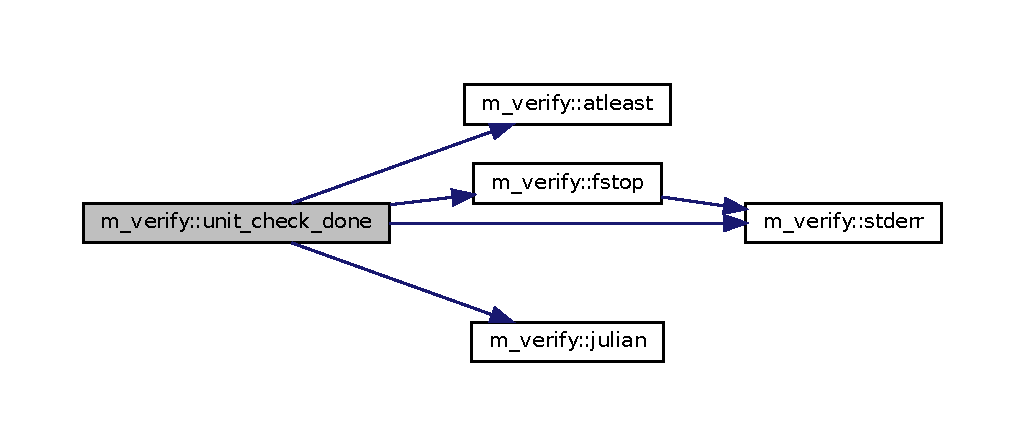
\includegraphics[width=350pt]{namespacem__verify_a0c0ed723b61b2cbbebb81fa91edd1941_cgraph}
\end{center}
\end{figure}
Here is the caller graph for this function\+:\nopagebreak
\begin{figure}[H]
\begin{center}
\leavevmode
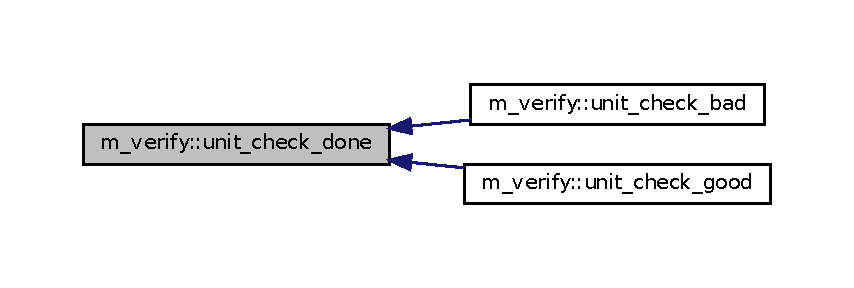
\includegraphics[width=350pt]{namespacem__verify_a0c0ed723b61b2cbbebb81fa91edd1941_icgraph}
\end{center}
\end{figure}
\mbox{\Hypertarget{namespacem__verify_a9d5ed59a1ac977dd7ab23e0d1fb54de4}\label{namespacem__verify_a9d5ed59a1ac977dd7ab23e0d1fb54de4}} 
\index{m\+\_\+verify@{m\+\_\+verify}!unit\+\_\+check\+\_\+good@{unit\+\_\+check\+\_\+good}}
\index{unit\+\_\+check\+\_\+good@{unit\+\_\+check\+\_\+good}!m\+\_\+verify@{m\+\_\+verify}}
\subsubsection{\texorpdfstring{unit\+\_\+check\+\_\+good()}{unit\_check\_good()}}
{\footnotesize\ttfamily subroutine, public m\+\_\+verify\+::unit\+\_\+check\+\_\+good (\begin{DoxyParamCaption}\item[{character(len=$\ast$), intent(in)}]{name,  }\item[{character(len=$\ast$), intent(in), optional}]{opts,  }\item[{character(len=$\ast$), intent(in), optional}]{msg }\end{DoxyParamCaption})}



\subsubsection*{N\+A\+ME}

unit\+\_\+check\+\_\+good(3f) -\/ \mbox{[}M\+\_\+verify\mbox{]} call command \char`\"{}goodbad N\+A\+M\+E good\char`\"{} (L\+I\+C\+E\+N\+SE\+:PD) 

\subsubsection*{S\+Y\+N\+O\+P\+S\+IS}

\begin{DoxyVerb}subroutine unit_check_good(name,opts,msg)

 character(len=*),intent(in)          :: name
 character(len=*),intent(in),optional :: opts
 character(len=*),intent(in),optional :: msg
\end{DoxyVerb}


\subsubsection*{D\+E\+S\+C\+R\+I\+P\+T\+I\+ON}

A shortcut for

call unit\+\_\+check(name,.true.) call unit\+\_\+check\+\_\+done(name,opts,msg)

\subsubsection*{E\+X\+A\+M\+P\+L\+ES}

Sample program\+:

program demo\+\_\+unit\+\_\+check\+\_\+good use M\+\_\+verify, only\+: unit\+\_\+check\+\_\+start, unit\+\_\+check\+\_\+done use M\+\_\+verify, only\+: unit\+\_\+check use M\+\_\+verify, only\+: unit\+\_\+check\+\_\+good, unit\+\_\+check\+\_\+bad

implicit none integer \+:\+: x x=10 call unit\+\_\+check\+\_\+start(\textquotesingle{}myroutine\textquotesingle{})

call unit\+\_\+check(\textquotesingle{}myroutine\textquotesingle{}, x.\+gt.\+3 ,\textquotesingle{}test if big enough\textquotesingle{}) call unit\+\_\+check(\textquotesingle{}myroutine\textquotesingle{}, x.\+lt.\+100 ,\textquotesingle{}test if small enough\textquotesingle{})

call unit\+\_\+check\+\_\+good(\textquotesingle{}myroutine\textquotesingle{},msg=\textquotesingle{}checks on \char`\"{}myroutine\char`\"{} \textquotesingle{})

end program demo\+\_\+unit\+\_\+check\+\_\+good

\subsubsection*{A\+U\+T\+H\+OR}

John S. Urban \subsubsection*{L\+I\+C\+E\+N\+SE}

Public Domain 

References unit\+\_\+check(), and unit\+\_\+check\+\_\+done().

Here is the call graph for this function\+:\nopagebreak
\begin{figure}[H]
\begin{center}
\leavevmode
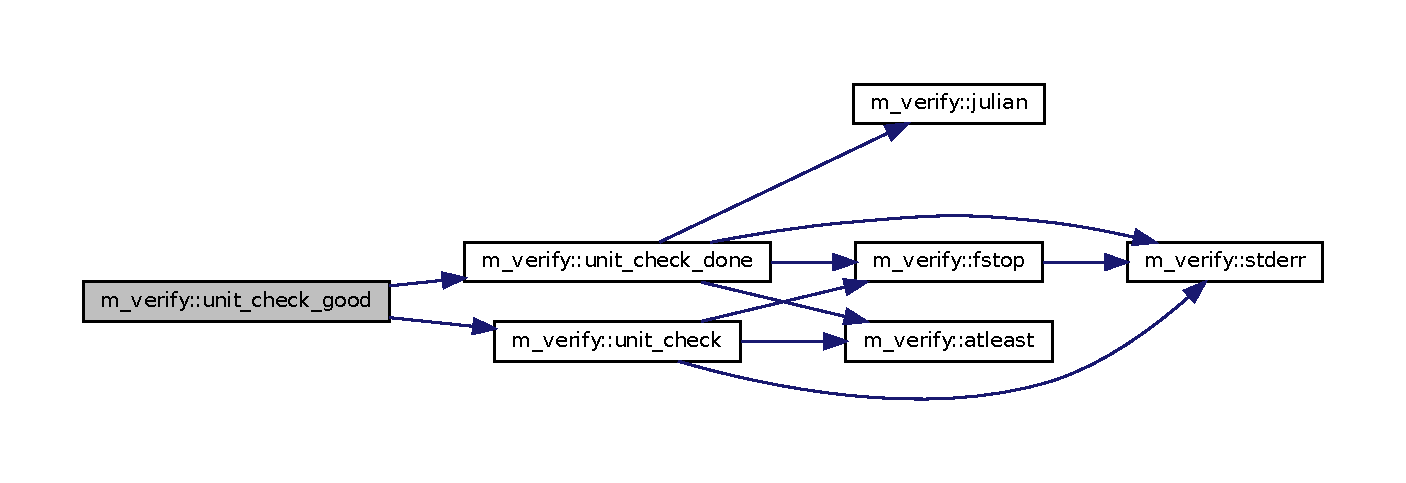
\includegraphics[width=350pt]{namespacem__verify_a9d5ed59a1ac977dd7ab23e0d1fb54de4_cgraph}
\end{center}
\end{figure}
\mbox{\Hypertarget{namespacem__verify_a74ea8b4574606c4f72e97b115375fc9b}\label{namespacem__verify_a74ea8b4574606c4f72e97b115375fc9b}} 
\index{m\+\_\+verify@{m\+\_\+verify}!unit\+\_\+check\+\_\+msg@{unit\+\_\+check\+\_\+msg}}
\index{unit\+\_\+check\+\_\+msg@{unit\+\_\+check\+\_\+msg}!m\+\_\+verify@{m\+\_\+verify}}
\subsubsection{\texorpdfstring{unit\+\_\+check\+\_\+msg()}{unit\_check\_msg()}}
{\footnotesize\ttfamily subroutine, public m\+\_\+verify\+::unit\+\_\+check\+\_\+msg (\begin{DoxyParamCaption}\item[{character(len=$\ast$), intent(in)}]{name,  }\item[{class($\ast$), intent(in), optional}]{g1,  }\item[{class($\ast$), intent(in), optional}]{g2,  }\item[{class($\ast$), intent(in), optional}]{g3,  }\item[{class($\ast$), intent(in), optional}]{g4,  }\item[{class($\ast$), intent(in), optional}]{g5,  }\item[{class($\ast$), intent(in), optional}]{g6,  }\item[{class($\ast$), intent(in), optional}]{g7,  }\item[{class($\ast$), intent(in), optional}]{g8,  }\item[{class($\ast$), intent(in), optional}]{g9 }\end{DoxyParamCaption})}



\subsubsection*{N\+A\+ME}

unit\+\_\+check\+\_\+msg(3f) -\/ \mbox{[}M\+\_\+verify\mbox{]} converts up to nine standard scalar values to a message for unit testing (L\+I\+C\+E\+N\+SE\+:PD) \subsubsection*{S\+Y\+N\+O\+P\+S\+IS}

function unit\+\_\+check\+\_\+msg(name,g1,g2g3,g4,g5,g6,g7,g8,g9)

character(len=$\ast$),intent(in) \+:\+: name class($\ast$),intent(in),optional \+:\+: g1,g2,g3,g4,g5,g6,g7,g8,g9 \subsubsection*{D\+E\+S\+C\+R\+I\+P\+T\+I\+ON}

unit\+\_\+check\+\_\+msg(3f) builds a string from up to nine scalar values and prints it to the error long.

\subsubsection*{O\+P\+T\+I\+O\+NS}

name name of unit being tested g\mbox{[}1-\/9\mbox{]} optional value to print the value of after the message. May be of type I\+N\+T\+E\+G\+ER, L\+O\+G\+I\+C\+AL, R\+E\+AL, D\+O\+U\+B\+L\+E\+P\+R\+E\+C\+I\+S\+I\+ON, C\+O\+M\+P\+L\+EX, or C\+H\+A\+R\+A\+C\+T\+ER.

\subsubsection*{E\+X\+A\+M\+P\+L\+ES}

Sample program\+:

program demo\+\_\+unit\+\_\+check\+\_\+msg use M\+\_\+verify, only \+: unit\+\_\+check\+\_\+start,unit\+\_\+check\+\_\+msg,unit\+\_\+check\+\_\+done implicit none character(len=\+:),allocatable \+:\+: pr

call unit\+\_\+check\+\_\+start(\textquotesingle{}myroutine\textquotesingle{}) call unit\+\_\+check\+\_\+msg(\textquotesingle{}myroutine\textquotesingle{},\textquotesingle{}H\+U\+G\+E(3f) integers\textquotesingle{},huge(0),\textquotesingle{}and real\textquotesingle{},huge(0.\+0),\textquotesingle{}and double\textquotesingle{},huge(0.\+0d0)) call unit\+\_\+check\+\_\+msg(\textquotesingle{}myroutine\textquotesingle{},\textquotesingle{}real \+:\textquotesingle{},huge(0.\+0),0.\+0,12345.\+6789,tiny(0.\+0) ) call unit\+\_\+check\+\_\+msg(\textquotesingle{}myroutine\textquotesingle{},\textquotesingle{}doubleprecision \+:\textquotesingle{},huge(0.\+0d0),0.\+0d0,12345.\+6789d0,tiny(0.\+0d0) ) call unit\+\_\+check\+\_\+msg(\textquotesingle{}myroutine\textquotesingle{},\textquotesingle{}complex \+:\textquotesingle{},cmplx(huge(0.\+0),tiny(0.\+0)) ) call unit\+\_\+check\+\_\+done(\textquotesingle{}myroutine\textquotesingle{})

end program demo\+\_\+unit\+\_\+check\+\_\+msg

\subsubsection*{A\+U\+T\+H\+OR}

John S. Urban \subsubsection*{L\+I\+C\+E\+N\+SE}

Public Domain 

References atleast(), and stderr().

Here is the call graph for this function\+:\nopagebreak
\begin{figure}[H]
\begin{center}
\leavevmode
\includegraphics[width=350pt]{namespacem__verify_a74ea8b4574606c4f72e97b115375fc9b_cgraph}
\end{center}
\end{figure}
\mbox{\Hypertarget{namespacem__verify_ad753d0a58dbc02c8917bf2b2aa3e1de7}\label{namespacem__verify_ad753d0a58dbc02c8917bf2b2aa3e1de7}} 
\index{m\+\_\+verify@{m\+\_\+verify}!unit\+\_\+check\+\_\+start@{unit\+\_\+check\+\_\+start}}
\index{unit\+\_\+check\+\_\+start@{unit\+\_\+check\+\_\+start}!m\+\_\+verify@{m\+\_\+verify}}
\subsubsection{\texorpdfstring{unit\+\_\+check\+\_\+start()}{unit\_check\_start()}}
{\footnotesize\ttfamily subroutine, public m\+\_\+verify\+::unit\+\_\+check\+\_\+start (\begin{DoxyParamCaption}\item[{character(len=$\ast$), intent(in)}]{name,  }\item[{character(len=$\ast$), intent(in), optional}]{options,  }\item[{character(len=$\ast$), intent(in), optional}]{msg }\end{DoxyParamCaption})}



\subsubsection*{N\+A\+ME}

unit\+\_\+check\+\_\+start(3f) -\/ \mbox{[}M\+\_\+verify\mbox{]} call command \char`\"{}goodbad N\+A\+M\+E start\char`\"{} and optionally set options (L\+I\+C\+E\+N\+SE\+:PD) 

\subsubsection*{S\+Y\+N\+O\+P\+S\+IS}

\begin{DoxyVerb}subroutine unit_check_start(name,options,msg)

 character(len=*),intent(in)          :: name
 character(len=*),intent(in),optional :: options
 character(len=*),intent(in),optional :: msg
\end{DoxyVerb}


\subsubsection*{D\+E\+S\+C\+R\+I\+P\+T\+I\+ON}

unit\+\_\+check\+\_\+start(3f) is an initialization command that by default calls the shell command

goodbad N\+A\+ME start \mbox{[}options\mbox{]}

The command can be changed by setting the environment variable U\+N\+I\+T\+\_\+\+C\+H\+E\+C\+K\+\_\+\+C\+O\+M\+M\+A\+ND or the global module variable U\+N\+I\+T\+\_\+\+C\+H\+E\+C\+K\+\_\+\+C\+O\+M\+M\+A\+ND. The environment variable overrides the global module variable.

By default if a unit\+\_\+check(3f) logical expression is false or the unit\+\_\+check\+\_\+bad(3f) procedure is called the program will be stopped.

This has the same effect as setting the environment variable M\+\_\+verify\+\_\+\+S\+T\+OP to \char`\"{}\+F\+A\+L\+S\+E\char`\"{} or the global module variable U\+N\+I\+T\+\_\+\+C\+H\+E\+C\+K\+\_\+\+K\+E\+E\+P\+\_\+\+G\+O\+I\+NG to .F\+A\+L\+SE. . Set the value to .true. and the program will continue even when tests fail.

\subsubsection*{O\+P\+T\+I\+O\+NS}

N\+A\+ME name of the shell command to execute. If blank, no command is executed. O\+P\+T\+I\+O\+NS pass additional options to the shell command

M\+SG print message

\subsubsection*{E\+X\+A\+M\+P\+L\+ES}

Sample program\+:

program demo\+\_\+unit\+\_\+check\+\_\+start use M\+\_\+verify, only\+: unit\+\_\+check\+\_\+start use M\+\_\+verify, only\+: unit\+\_\+check use M\+\_\+verify, only\+: unit\+\_\+check\+\_\+done

implicit none integer \+:\+: ival call unit\+\_\+check\+\_\+start(\textquotesingle{}myroutine\textquotesingle{}) ! the goodbad(1) command called here takes many options ! used to build an S\+Q\+Lite3 entry call unit\+\_\+check\+\_\+start(\textquotesingle{}myroutine\+\_\+long\textquotesingle{},\textquotesingle{} \& \& -\/section 3 \& \& -\/library lib\+G\+PF \& \& -\/filename {\ttfamily pwd}/\+M\+\_\+verify.FF \& \& -\/documentation y \& \& -\/ufpp y \& \& -\/ccall n \& \& -\/archive G\+P\+F.\+a \& \& \textquotesingle{})

ival=10 call unit\+\_\+check(\textquotesingle{}myroutine\textquotesingle{}, ival.\+gt.\+3 , msg=\textquotesingle{}test if big enough\textquotesingle{}) call unit\+\_\+check(\textquotesingle{}myroutine\textquotesingle{}, ival.\+lt.\+100 , msg=\textquotesingle{}test if small enough\textquotesingle{})

call unit\+\_\+check\+\_\+done(\textquotesingle{}myroutine\textquotesingle{},msg=\textquotesingle{}completed checks of \char`\"{}myroutine\char`\"{}\textquotesingle{})

end program demo\+\_\+unit\+\_\+check\+\_\+start

\subsubsection*{A\+U\+T\+H\+OR}

John S. Urban \subsubsection*{L\+I\+C\+E\+N\+SE}

Public Domain 

References atleast(), clicks, duration, ifailed\+\_\+g, ipassed\+\_\+g, julian(), stderr(), unit\+\_\+check\+\_\+command, and unit\+\_\+check\+\_\+keep\+\_\+going.

Here is the call graph for this function\+:\nopagebreak
\begin{figure}[H]
\begin{center}
\leavevmode
\includegraphics[width=333pt]{namespacem__verify_ad753d0a58dbc02c8917bf2b2aa3e1de7_cgraph}
\end{center}
\end{figure}


\subsection{Variable Documentation}
\mbox{\Hypertarget{namespacem__verify_af97c7f92394811bec5fed506fdfab67d}\label{namespacem__verify_af97c7f92394811bec5fed506fdfab67d}} 
\index{m\+\_\+verify@{m\+\_\+verify}!clicks@{clicks}}
\index{clicks@{clicks}!m\+\_\+verify@{m\+\_\+verify}}
\subsubsection{\texorpdfstring{clicks}{clicks}}
{\footnotesize\ttfamily integer, save m\+\_\+verify\+::clicks =0.\+0d0\hspace{0.3cm}{\ttfamily [private]}}

\mbox{\Hypertarget{namespacem__verify_a0f87b43bebf70897f9ec711be3f01839}\label{namespacem__verify_a0f87b43bebf70897f9ec711be3f01839}} 
\index{m\+\_\+verify@{m\+\_\+verify}!debug@{debug}}
\index{debug@{debug}!m\+\_\+verify@{m\+\_\+verify}}
\subsubsection{\texorpdfstring{debug}{debug}}
{\footnotesize\ttfamily logical, save, public m\+\_\+verify\+::debug =.false.}

\mbox{\Hypertarget{namespacem__verify_a77729c599fbd8aed6075a05fb3c38146}\label{namespacem__verify_a77729c599fbd8aed6075a05fb3c38146}} 
\index{m\+\_\+verify@{m\+\_\+verify}!duration@{duration}}
\index{duration@{duration}!m\+\_\+verify@{m\+\_\+verify}}
\subsubsection{\texorpdfstring{duration}{duration}}
{\footnotesize\ttfamily real(kind=\mbox{\hyperlink{namespacem__verify_a7f6aa94b09b3824bc5c15bc74e757d6b}{realtime}}), save m\+\_\+verify\+::duration =0.\+0d0\hspace{0.3cm}{\ttfamily [private]}}

\mbox{\Hypertarget{namespacem__verify_a458c47b6b47738f8ebadddb4a944d0e0}\label{namespacem__verify_a458c47b6b47738f8ebadddb4a944d0e0}} 
\index{m\+\_\+verify@{m\+\_\+verify}!exit\+\_\+failure@{exit\+\_\+failure}}
\index{exit\+\_\+failure@{exit\+\_\+failure}!m\+\_\+verify@{m\+\_\+verify}}
\subsubsection{\texorpdfstring{exit\+\_\+failure}{exit\_failure}}
{\footnotesize\ttfamily integer, parameter, public m\+\_\+verify\+::exit\+\_\+failure =1}

\mbox{\Hypertarget{namespacem__verify_a278d7a36f55fac875e4f94bc893447fe}\label{namespacem__verify_a278d7a36f55fac875e4f94bc893447fe}} 
\index{m\+\_\+verify@{m\+\_\+verify}!exit\+\_\+success@{exit\+\_\+success}}
\index{exit\+\_\+success@{exit\+\_\+success}!m\+\_\+verify@{m\+\_\+verify}}
\subsubsection{\texorpdfstring{exit\+\_\+success}{exit\_success}}
{\footnotesize\ttfamily integer, parameter, public m\+\_\+verify\+::exit\+\_\+success =0}

\mbox{\Hypertarget{namespacem__verify_ab18f1875be62b6aa1e101894358b617f}\label{namespacem__verify_ab18f1875be62b6aa1e101894358b617f}} 
\index{m\+\_\+verify@{m\+\_\+verify}!ifailed\+\_\+g@{ifailed\+\_\+g}}
\index{ifailed\+\_\+g@{ifailed\+\_\+g}!m\+\_\+verify@{m\+\_\+verify}}
\subsubsection{\texorpdfstring{ifailed\+\_\+g}{ifailed\_g}}
{\footnotesize\ttfamily integer, save m\+\_\+verify\+::ifailed\+\_\+g =0\hspace{0.3cm}{\ttfamily [private]}}

\mbox{\Hypertarget{namespacem__verify_a7014b3aa584eb29266bf52fc6e03e6ed}\label{namespacem__verify_a7014b3aa584eb29266bf52fc6e03e6ed}} 
\index{m\+\_\+verify@{m\+\_\+verify}!io\+\_\+debug@{io\+\_\+debug}}
\index{io\+\_\+debug@{io\+\_\+debug}!m\+\_\+verify@{m\+\_\+verify}}
\subsubsection{\texorpdfstring{io\+\_\+debug}{io\_debug}}
{\footnotesize\ttfamily integer, save, public m\+\_\+verify\+::io\+\_\+debug =E\+R\+R\+O\+R\+\_\+\+U\+N\+IT}

\mbox{\Hypertarget{namespacem__verify_ada62999b3a1ef795c335deccac28cda5}\label{namespacem__verify_ada62999b3a1ef795c335deccac28cda5}} 
\index{m\+\_\+verify@{m\+\_\+verify}!ipassed\+\_\+g@{ipassed\+\_\+g}}
\index{ipassed\+\_\+g@{ipassed\+\_\+g}!m\+\_\+verify@{m\+\_\+verify}}
\subsubsection{\texorpdfstring{ipassed\+\_\+g}{ipassed\_g}}
{\footnotesize\ttfamily integer, save m\+\_\+verify\+::ipassed\+\_\+g =0\hspace{0.3cm}{\ttfamily [private]}}

\mbox{\Hypertarget{namespacem__verify_aa827fd6225334c65efe89d1d0af79efa}\label{namespacem__verify_aa827fd6225334c65efe89d1d0af79efa}} 
\index{m\+\_\+verify@{m\+\_\+verify}!no\+\_\+news\+\_\+is\+\_\+good\+\_\+news@{no\+\_\+news\+\_\+is\+\_\+good\+\_\+news}}
\index{no\+\_\+news\+\_\+is\+\_\+good\+\_\+news@{no\+\_\+news\+\_\+is\+\_\+good\+\_\+news}!m\+\_\+verify@{m\+\_\+verify}}
\subsubsection{\texorpdfstring{no\+\_\+news\+\_\+is\+\_\+good\+\_\+news}{no\_news\_is\_good\_news}}
{\footnotesize\ttfamily logical, save, public m\+\_\+verify\+::no\+\_\+news\+\_\+is\+\_\+good\+\_\+news =.false.}

\mbox{\Hypertarget{namespacem__verify_a7f6aa94b09b3824bc5c15bc74e757d6b}\label{namespacem__verify_a7f6aa94b09b3824bc5c15bc74e757d6b}} 
\index{m\+\_\+verify@{m\+\_\+verify}!realtime@{realtime}}
\index{realtime@{realtime}!m\+\_\+verify@{m\+\_\+verify}}
\subsubsection{\texorpdfstring{realtime}{realtime}}
{\footnotesize\ttfamily integer, parameter, public m\+\_\+verify\+::realtime =kind(0.\+0d0)}

\mbox{\Hypertarget{namespacem__verify_a425cad68370e8552495e1838b2e34734}\label{namespacem__verify_a425cad68370e8552495e1838b2e34734}} 
\index{m\+\_\+verify@{m\+\_\+verify}!stop\+\_\+g@{stop\+\_\+g}}
\index{stop\+\_\+g@{stop\+\_\+g}!m\+\_\+verify@{m\+\_\+verify}}
\subsubsection{\texorpdfstring{stop\+\_\+g}{stop\_g}}
{\footnotesize\ttfamily logical, save m\+\_\+verify\+::stop\+\_\+g =.true.\hspace{0.3cm}{\ttfamily [private]}}

\mbox{\Hypertarget{namespacem__verify_aaa3c6dfa94a9414592071525036020d4}\label{namespacem__verify_aaa3c6dfa94a9414592071525036020d4}} 
\index{m\+\_\+verify@{m\+\_\+verify}!unit\+\_\+check\+\_\+command@{unit\+\_\+check\+\_\+command}}
\index{unit\+\_\+check\+\_\+command@{unit\+\_\+check\+\_\+command}!m\+\_\+verify@{m\+\_\+verify}}
\subsubsection{\texorpdfstring{unit\+\_\+check\+\_\+command}{unit\_check\_command}}
{\footnotesize\ttfamily character(len=4096), public m\+\_\+verify\+::unit\+\_\+check\+\_\+command =\textquotesingle{}goodbad\textquotesingle{}}

\mbox{\Hypertarget{namespacem__verify_a434af7c4d380da5b85d49dc07466dde8}\label{namespacem__verify_a434af7c4d380da5b85d49dc07466dde8}} 
\index{m\+\_\+verify@{m\+\_\+verify}!unit\+\_\+check\+\_\+keep\+\_\+going@{unit\+\_\+check\+\_\+keep\+\_\+going}}
\index{unit\+\_\+check\+\_\+keep\+\_\+going@{unit\+\_\+check\+\_\+keep\+\_\+going}!m\+\_\+verify@{m\+\_\+verify}}
\subsubsection{\texorpdfstring{unit\+\_\+check\+\_\+keep\+\_\+going}{unit\_check\_keep\_going}}
{\footnotesize\ttfamily logical, save, public m\+\_\+verify\+::unit\+\_\+check\+\_\+keep\+\_\+going =.false.}

\mbox{\Hypertarget{namespacem__verify_afe37222ddb2a9470e1a0e9c40e2dcce3}\label{namespacem__verify_afe37222ddb2a9470e1a0e9c40e2dcce3}} 
\index{m\+\_\+verify@{m\+\_\+verify}!unit\+\_\+check\+\_\+level@{unit\+\_\+check\+\_\+level}}
\index{unit\+\_\+check\+\_\+level@{unit\+\_\+check\+\_\+level}!m\+\_\+verify@{m\+\_\+verify}}
\subsubsection{\texorpdfstring{unit\+\_\+check\+\_\+level}{unit\_check\_level}}
{\footnotesize\ttfamily integer, save, public m\+\_\+verify\+::unit\+\_\+check\+\_\+level =0}

\mbox{\Hypertarget{namespacem__verify_a65569c8b4be204251ba14430ad18372d}\label{namespacem__verify_a65569c8b4be204251ba14430ad18372d}} 
\index{m\+\_\+verify@{m\+\_\+verify}!unit\+\_\+check\+\_\+lun@{unit\+\_\+check\+\_\+lun}}
\index{unit\+\_\+check\+\_\+lun@{unit\+\_\+check\+\_\+lun}!m\+\_\+verify@{m\+\_\+verify}}
\subsubsection{\texorpdfstring{unit\+\_\+check\+\_\+lun}{unit\_check\_lun}}
{\footnotesize\ttfamily integer, save, public m\+\_\+verify\+::unit\+\_\+check\+\_\+lun =E\+R\+R\+O\+R\+\_\+\+U\+N\+IT}


\chapter{Data Type Documentation}
\hypertarget{interfacem__journal_1_1journal}{}\section{m\+\_\+journal\+:\+:journal Interface Reference}
\label{interfacem__journal_1_1journal}\index{m\+\_\+journal\+::journal@{m\+\_\+journal\+::journal}}


\subsubsection*{N\+A\+ME}

journal(3f) -\/ \mbox{[}M\+\_\+journal\mbox{]} provides public message routine, no paging or graphic mode change (L\+I\+C\+E\+N\+SE\+:PD) \subsubsection*{S\+Y\+N\+O\+P\+S\+IS} 


\subsection*{Private Member Functions}
\begin{DoxyCompactItemize}
\item 
subroutine \mbox{\hyperlink{interfacem__journal_1_1journal_acdde0ed4590797094f797514820e34fc}{flush\+\_\+trail}} ()
\item 
subroutine \mbox{\hyperlink{interfacem__journal_1_1journal_a1cb40f602a1e1c546bce71652a779d31}{write\+\_\+message\+\_\+only}} (message)
\item 
subroutine \mbox{\hyperlink{interfacem__journal_1_1journal_ae6136e918d4383d1c463c536a3eb814a}{where\+\_\+write\+\_\+message\+\_\+all}} (where, g0, g1, g2, g3, g4, g5, g6, g7, g8, g9, nospace)
\begin{DoxyCompactList}\small\item\em \subsubsection*{N\+A\+ME}

where\+\_\+write\+\_\+message\+\_\+all(3f) -\/ \mbox{[}M\+\_\+journal\mbox{]} converts any standard scalar type to a string and calls journal(3f) (L\+I\+C\+E\+N\+SE\+:PD) \subsubsection*{S\+Y\+N\+O\+P\+S\+IS}\end{DoxyCompactList}\item 
subroutine \mbox{\hyperlink{interfacem__journal_1_1journal_a78f9c4a4314847963a2feae798ff54c1}{set\+\_\+stdout\+\_\+lun}} (iounit)
\end{DoxyCompactItemize}


\subsection{Detailed Description}
\subsubsection*{N\+A\+ME}

journal(3f) -\/ \mbox{[}M\+\_\+journal\mbox{]} provides public message routine, no paging or graphic mode change (L\+I\+C\+E\+N\+SE\+:PD) \subsubsection*{S\+Y\+N\+O\+P\+S\+IS}

subroutine journal(\mbox{[}where,\mbox{]},\mbox{[}\+V\+A\+L\+U\+E(s)\mbox{]})

character(len=$\ast$),intent(in) \+:\+: where character(len=$\ast$)$\vert$real$\vert$integer$\vert$doubleprecision$\vert$complex,optional \+:\+: g1,g2,g3,g4,g5,g6,g7,g8,g9

W\+R\+I\+TE M\+E\+S\+S\+A\+G\+ES basic messages

call journal(where,\mbox{[}\+V\+A\+L\+U\+E(\+S)\mbox{]}) call journal(message) \# a shortcut for \char`\"{}call journal(\textquotesingle{}sc\textquotesingle{},message)\char`\"{}\+: O\+P\+EN OR C\+L\+O\+SE T\+R\+A\+IL F\+I\+LE trail file

call journal(\textquotesingle{}O\textquotesingle{},trailfile\+\_\+name) \# open trail file call journal(\textquotesingle{}O\textquotesingle{},\textquotesingle{}\textquotesingle{}) \# close trail file S\+ET O\+U\+T\+P\+UT T\+I\+ME P\+R\+E\+F\+IX set the function display format for timestamps. See the N\+O\+W(3f) procedure for allowable timestamp macros

call journal(\textquotesingle{}\textquotesingle{},time\+\_\+stamp\+\_\+prefix\+\_\+specification)

M\+O\+D\+ES

Turn on/off writing D\+E\+B\+UG messages to trail file

call journal(\textquotesingle{}$>$\textquotesingle{},\textquotesingle{}debug on\textquotesingle{}) \# turn on debug mode call journal(\textquotesingle{}$<$\textquotesingle{},\textquotesingle{}debug off\textquotesingle{}) \# turn off debug mode

A\+S\+S\+I\+GN S\+T\+D\+O\+UT TO AN A\+L\+T\+E\+R\+N\+A\+TE F\+I\+LE change stdout to iunit and open filename; or close unit and go back to stdout if filename=\textquotesingle{}\textquotesingle{}

call journal(iunit,filename)

change stdout to iunit to use a file already open

call journal(iunit)

\subsubsection*{D\+E\+S\+C\+R\+I\+P\+T\+I\+ON}

\begin{DoxyVerb}If a user procedure is used for outputting messages instead of calling
WRITE(3f) it is easy to provide control of when messages are printed
(ie. a "verbose" mode, or "quite" mode), creating files to replay
program execution, duplicating output, ...
\end{DoxyVerb}


\subsubsection*{O\+P\+T\+I\+O\+NS}

W\+H\+E\+RE indicates where messages are written. A combination of the following characters can be used...

Usually one of these to write to the standard output files ...

S write to stdout or iounit set with journal(unit) or journal(unit,filename). E write to stderr

And one of these to write to trail file (ignore if no trail file defined) ...

C write to trail file as a comment (if file is open) Writing output \char`\"{}as a comment\char`\"{} means it is preceded by a pound(\#) character. T write to trail file (if file is open)

Usually used by itself

D write to trail file as a comment with \char`\"{}\+D\+E\+B\+U\+G\+:\char`\"{} prefix in front of message (if file is open) if debug mode is on. Write to stdout if no trail file and debug mode is on.

Modifier for S$\vert$\+E$\vert$\+C$\vert$\+T$\vert$D specifiers


\begin{DoxyItemize}
\item subsequent files are written to with advance=\textquotesingle{}no\textquotesingle{}. Position is important. \textquotesingle{}+sc\textquotesingle{} does an advance=\textquotesingle{}no\textquotesingle{} on both files, \textquotesingle{}s+c\textquotesingle{} only does the advance=\textquotesingle{}no\textquotesingle{} for the trail file.
\end{DoxyItemize}

Mode changing options used by themselves\+:

$>$ turn off debug messages $<$ turn on debug messages O open trail file using value of \char`\"{}message\char`\"{} parameter or close trail file if no filename or a blank filename. A Auxiliary programs that also want to write to the current log file (a2b, z2a, ...) call this routine to see if there is a trail file being generated and then add to it so that a program like ush(1f) can call the auxiliary programs and still just generate one log file, but if the auxiliary program is used as a stand-\/alone program no trail is generated.

V\+A\+L\+U\+E\+S(\+S) message to write to stdout, stderr, and the trail file. a numeric or character value to optionally be appended to the message. Up to nine values are allowed. The W\+H\+E\+RE field is required if values are added. F\+I\+L\+E\+N\+A\+ME when W\+H\+E\+RE=\char`\"{}\+O\char`\"{} to turn the trail file on or off, the \char`\"{}message\char`\"{} field becomes the trail filename to open. If blank, writing to the trail file is turned off. T\+F\+O\+R\+M\+AT when W\+H\+E\+RE=\char`\"{}\%\char`\"{} the message is treated as a time format specification as described under now(3f).

\subsubsection*{E\+X\+A\+M\+P\+LE}

Sample program\+:

program demo\+\_\+journal use M\+\_\+journal, only \+: journal !! B\+A\+S\+IC U\+S\+A\+GE call journal(\textquotesingle{}write to standard output as-\/is, and trail file as a comment if open\textquotesingle{}) ! since we have not opened a trail file yet, only stdout will display output call journal(\textquotesingle{}c\textquotesingle{},\textquotesingle{}ignored, as trail file is not open\textquotesingle{}) ! now open trail file \char`\"{}trail\char`\"{} call journal(\textquotesingle{}o\textquotesingle{},\textquotesingle{}trail\textquotesingle{}) call journal(\textquotesingle{}sc\textquotesingle{},\textquotesingle{}same thing except now trail file is open\textquotesingle{}) ! only write to trail file if open call journal(\textquotesingle{}c\textquotesingle{},\textquotesingle{}not ignored, as trail file is open. Written with \# suffix\textquotesingle{}) call journal(\textquotesingle{}t\textquotesingle{},\textquotesingle{}not ignored, as trail file is open. Written as-\/is\textquotesingle{}) ! turn off trail file call journal(\textquotesingle{}o\textquotesingle{},\textquotesingle{}\textquotesingle{}) end program demo\+\_\+journal

Adding intrinsic scalar values to the message\+:

program test\+\_\+journal use M\+\_\+journal, only\+: journal implicit none call journal(\textquotesingle{}S\textquotesingle{},\textquotesingle{}This is a test with no optional value\textquotesingle{}) call journal(\textquotesingle{}S\textquotesingle{},\textquotesingle{}This is a test with a logical value\textquotesingle{},.true.) call journal(\textquotesingle{}S\textquotesingle{},\textquotesingle{}This is a test with a double value\textquotesingle{},1234567890.\+123456789d0) call journal(\textquotesingle{}S\textquotesingle{},\textquotesingle{}This is a test with a real value\textquotesingle{},1234567890.\+123456789) call journal(\textquotesingle{}S\textquotesingle{},\textquotesingle{}This is a test with an integer value\textquotesingle{},1234567890) call journal(\textquotesingle{}S\+T\+DC\textquotesingle{},\textquotesingle{}This is a test using S\+T\+DC\textquotesingle{},1234567890) call journal(\textquotesingle{}stdc\textquotesingle{},\textquotesingle{}This is a test using stdc\textquotesingle{},1234567890) call journal(\textquotesingle{}o\textquotesingle{},\textquotesingle{}journal.\+txt\textquotesingle{}) ! open trail file call journal(\textquotesingle{}S\textquotesingle{},1,12.\+34,56789.\+111111111d0,.false.,\textquotesingle{}a bunch of values\textquotesingle{}) ! the combinations that make sense call journal(\textquotesingle{}st\textquotesingle{},\textquotesingle{}stdout and trail\textquotesingle{}) call journal(\textquotesingle{}s\textquotesingle{} ,\textquotesingle{}stdout only\textquotesingle{}) call journal(\textquotesingle{}t\textquotesingle{} ,\textquotesingle{}trail only\textquotesingle{}) call journal(\textquotesingle{}sc\textquotesingle{},\textquotesingle{}stdout and trail\+\_\+comment\textquotesingle{}) call journal(\textquotesingle{}c\textquotesingle{} ,\textquotesingle{}trail\+\_\+comment only \textquotesingle{}) call journal(\textquotesingle{}d\textquotesingle{} ,\textquotesingle{}debug only\textquotesingle{}) call journal(\textquotesingle{}e\textquotesingle{} ,\textquotesingle{}stderr only\textquotesingle{}) call journal(\textquotesingle{}o\textquotesingle{} ,\textquotesingle{} \textquotesingle{}) ! closing trail file end program test\+\_\+journal

program testit ! this is a utility program that calls the module routines. It is typically built using ccall(1). use M\+\_\+journal, only \+: journal character(len=\+:),allocatable \+:\+: time\+\_\+stamp\+\_\+prefix call journal(\textquotesingle{}s\textquotesingle{},\textquotesingle{}-\/-\/-\/-\/-\/-\/-\/-\/-\/-\/-\/-\/-\/-\/-\/-\/-\/-\/-\/-\/-\/-\/-\/-\/-\/-\/-\/-\/-\/-\/-\/-\/-\/-\/-\/-\/-\/-\/-\/-\/-\/-\/-\/-\/-\/-\/-\/-\/-\/-\/-\/-\/-\/-\/-\/-\/-\/-\/-\/-\/-\/-\/-\/-\/-\/-\/-\/-\/-\/-\/-\/-\/-\/-\/-\/-\/-\/---\textquotesingle{}) call journal(\textquotesingle{}s\textquotesingle{},\textquotesingle{}S\+I\+M\+P\+LE W\+R\+I\+T\+ES\textquotesingle{}) call one() call two() call journal(\textquotesingle{}sc\textquotesingle{},\textquotesingle{}called O\+N\+E() and T\+W\+O() but did not generate a log file\textquotesingle{}) call journal(\textquotesingle{}s\textquotesingle{},\textquotesingle{}-\/-\/-\/-\/-\/-\/-\/-\/-\/-\/-\/-\/-\/-\/-\/-\/-\/-\/-\/-\/-\/-\/-\/-\/-\/-\/-\/-\/-\/-\/-\/-\/-\/-\/-\/-\/-\/-\/-\/-\/-\/-\/-\/-\/-\/-\/-\/-\/-\/-\/-\/-\/-\/-\/-\/-\/-\/-\/-\/-\/-\/-\/-\/-\/-\/-\/-\/-\/-\/-\/-\/-\/-\/-\/-\/-\/-\/---\textquotesingle{}) call journal(\textquotesingle{}s\textquotesingle{},\textquotesingle{}S\+I\+M\+P\+LE W\+R\+I\+T\+ES W\+I\+TH L\+OG F\+I\+LE\textquotesingle{}) call journal(\textquotesingle{}o\textquotesingle{},\textquotesingle{}journal.\+txt\textquotesingle{}) ! open trail file call one() call two() call journal(\textquotesingle{}sc\textquotesingle{},\textquotesingle{}called O\+N\+E() and T\+W\+O() and generated log file journal.\+txt\textquotesingle{}) call journal(\textquotesingle{}\textquotesingle{},\textquotesingle{}journal.\+txt\textquotesingle{}) ! close trail file call journal(\textquotesingle{}s\textquotesingle{},\textquotesingle{}-\/-\/-\/-\/-\/-\/-\/-\/-\/-\/-\/-\/-\/-\/-\/-\/-\/-\/-\/-\/-\/-\/-\/-\/-\/-\/-\/-\/-\/-\/-\/-\/-\/-\/-\/-\/-\/-\/-\/-\/-\/-\/-\/-\/-\/-\/-\/-\/-\/-\/-\/-\/-\/-\/-\/-\/-\/-\/-\/-\/-\/-\/-\/-\/-\/-\/-\/-\/-\/-\/-\/-\/-\/-\/-\/-\/-\/---\textquotesingle{}) call journal(\textquotesingle{}s\textquotesingle{},\textquotesingle{}S\+I\+M\+P\+LE W\+R\+I\+T\+ES W\+I\+TH T\+I\+M\+I\+NG I\+N\+F\+O\+R\+M\+A\+T\+I\+ON\textquotesingle{}) time\+\_\+stamp\+\_\+prefix=\textquotesingle{}C\+P\+U\+\_\+\+T\+I\+ME=c\+:C\+A\+L\+LS=C\+:S\+I\+N\+CE=S\+:b\textquotesingle{} ! change time prefix call journal(\textquotesingle{}\textquotesingle{},time\+\_\+stamp\+\_\+prefix) ! set a time prefix in front of messages call journal(\textquotesingle{}o\textquotesingle{},\textquotesingle{}timed.\+txt\textquotesingle{}) ! open trail file call one() call two() call journal(\textquotesingle{}sc\textquotesingle{},\textquotesingle{}called O\+N\+E() and T\+W\+O() and generate log file timed.\+txt\textquotesingle{}) call journal(\textquotesingle{}\textquotesingle{},\textquotesingle{}timed.\+txt\textquotesingle{}) ! close trail file call journal(\textquotesingle{}\textquotesingle{},\textquotesingle{}\textquotesingle{}) ! turn off time prefix call journal(\textquotesingle{}o\textquotesingle{},\textquotesingle{}timed.\+txt\textquotesingle{}) ! open trail file call journal(\textquotesingle{}s\textquotesingle{},\textquotesingle{}-\/-\/-\/-\/-\/-\/-\/-\/-\/-\/-\/-\/-\/-\/-\/-\/-\/-\/-\/-\/-\/-\/-\/-\/-\/-\/-\/-\/-\/-\/-\/-\/-\/-\/-\/-\/-\/-\/-\/-\/-\/-\/-\/-\/-\/-\/-\/-\/-\/-\/-\/-\/-\/-\/-\/-\/-\/-\/-\/-\/-\/-\/-\/-\/-\/-\/-\/-\/-\/-\/-\/-\/-\/-\/-\/-\/-\/---\textquotesingle{})

contains

subroutine two() call journal(\textquotesingle{}Entered subroutine two\textquotesingle{}) call journal(\textquotesingle{}Exited subroutine two\textquotesingle{}) end subroutine two

subroutine one() call journal(\textquotesingle{}Entered subroutine one\textquotesingle{}) sum=-\/\+H\+U\+GE(1.\+0) do i=1,10000000 sum=sum+sqrt(real(i)) enddo write($\ast$,$\ast$)\textquotesingle{}S\+UM=\textquotesingle{},sum call journal(\textquotesingle{}Exited subroutine one\textquotesingle{}) end subroutine one

end program testit

\subsubsection*{A\+U\+T\+H\+OR}

John S. Urban

\subsubsection*{L\+I\+C\+E\+N\+SE}

Public Domain 

\subsection{Member Function/\+Subroutine Documentation}
\mbox{\Hypertarget{interfacem__journal_1_1journal_acdde0ed4590797094f797514820e34fc}\label{interfacem__journal_1_1journal_acdde0ed4590797094f797514820e34fc}} 
\index{m\+\_\+journal\+::journal@{m\+\_\+journal\+::journal}!flush\+\_\+trail@{flush\+\_\+trail}}
\index{flush\+\_\+trail@{flush\+\_\+trail}!m\+\_\+journal\+::journal@{m\+\_\+journal\+::journal}}
\subsubsection{\texorpdfstring{flush\+\_\+trail()}{flush\_trail()}}
{\footnotesize\ttfamily subroutine m\+\_\+journal\+::journal\+::flush\+\_\+trail (\begin{DoxyParamCaption}{ }\end{DoxyParamCaption})\hspace{0.3cm}{\ttfamily [private]}}

\mbox{\Hypertarget{interfacem__journal_1_1journal_a78f9c4a4314847963a2feae798ff54c1}\label{interfacem__journal_1_1journal_a78f9c4a4314847963a2feae798ff54c1}} 
\index{m\+\_\+journal\+::journal@{m\+\_\+journal\+::journal}!set\+\_\+stdout\+\_\+lun@{set\+\_\+stdout\+\_\+lun}}
\index{set\+\_\+stdout\+\_\+lun@{set\+\_\+stdout\+\_\+lun}!m\+\_\+journal\+::journal@{m\+\_\+journal\+::journal}}
\subsubsection{\texorpdfstring{set\+\_\+stdout\+\_\+lun()}{set\_stdout\_lun()}}
{\footnotesize\ttfamily subroutine m\+\_\+journal\+::journal\+::set\+\_\+stdout\+\_\+lun (\begin{DoxyParamCaption}\item[{integer, intent(in)}]{iounit }\end{DoxyParamCaption})\hspace{0.3cm}{\ttfamily [private]}}

\mbox{\Hypertarget{interfacem__journal_1_1journal_ae6136e918d4383d1c463c536a3eb814a}\label{interfacem__journal_1_1journal_ae6136e918d4383d1c463c536a3eb814a}} 
\index{m\+\_\+journal\+::journal@{m\+\_\+journal\+::journal}!where\+\_\+write\+\_\+message\+\_\+all@{where\+\_\+write\+\_\+message\+\_\+all}}
\index{where\+\_\+write\+\_\+message\+\_\+all@{where\+\_\+write\+\_\+message\+\_\+all}!m\+\_\+journal\+::journal@{m\+\_\+journal\+::journal}}
\subsubsection{\texorpdfstring{where\+\_\+write\+\_\+message\+\_\+all()}{where\_write\_message\_all()}}
{\footnotesize\ttfamily subroutine m\+\_\+journal\+::journal\+::where\+\_\+write\+\_\+message\+\_\+all (\begin{DoxyParamCaption}\item[{character(len=$\ast$), intent(in)}]{where,  }\item[{class($\ast$), intent(in)}]{g0,  }\item[{class($\ast$), intent(in), optional}]{g1,  }\item[{class($\ast$), intent(in), optional}]{g2,  }\item[{class($\ast$), intent(in), optional}]{g3,  }\item[{class($\ast$), intent(in), optional}]{g4,  }\item[{class($\ast$), intent(in), optional}]{g5,  }\item[{class($\ast$), intent(in), optional}]{g6,  }\item[{class($\ast$), intent(in), optional}]{g7,  }\item[{class($\ast$), intent(in), optional}]{g8,  }\item[{class($\ast$), intent(in), optional}]{g9,  }\item[{logical, intent(in), optional}]{nospace }\end{DoxyParamCaption})\hspace{0.3cm}{\ttfamily [private]}}



\subsubsection*{N\+A\+ME}

where\+\_\+write\+\_\+message\+\_\+all(3f) -\/ \mbox{[}M\+\_\+journal\mbox{]} converts any standard scalar type to a string and calls journal(3f) (L\+I\+C\+E\+N\+SE\+:PD) \subsubsection*{S\+Y\+N\+O\+P\+S\+IS}

subroutine where\+\_\+write\+\_\+message\+\_\+all(where,g0,g1,g2g3,g4,g5,g6,g7,g8,g9,nospace)

character(len=$\ast$),intent(in) \+:\+: where class($\ast$),intent(in) \+:\+: g0 class($\ast$),intent(in),optional \+:\+: g1,g2,g3,g4,g5,g6,g7,g8,g9 logical,intent(in),optional \+:\+: nospace

\subsubsection*{D\+E\+S\+C\+R\+I\+P\+T\+I\+ON}

where\+\_\+write\+\_\+message\+\_\+all(3f) builds and writes a space-\/separated string from up to nine scalar values.

\subsubsection*{O\+P\+T\+I\+O\+NS}

\begin{DoxyVerb}where    string designating where to write message, as with journal(3f)
g0       value to print. May
         be of type INTEGER, LOGICAL, REAL, DOUBLEPRECISION, COMPLEX,
         or CHARACTER.
g[1-9]   optional additional values to print the value of after g0.
nospace  if nospace=.true., then no spaces are added between values
\end{DoxyVerb}
 \subsubsection*{R\+E\+T\+U\+R\+NS}

where\+\_\+write\+\_\+message\+\_\+all description to print

\subsubsection*{E\+X\+A\+M\+P\+L\+ES}

Sample program\+:

program demo\+\_\+wm\+\_\+all use M\+\_\+journal, only \+: where\+\_\+write\+\_\+message\+\_\+all implicit none end program program demo\+\_\+wm\+\_\+all \subsubsection*{A\+U\+T\+H\+OR}

John S. Urban \subsubsection*{L\+I\+C\+E\+N\+SE}

Public Domain \mbox{\Hypertarget{interfacem__journal_1_1journal_a1cb40f602a1e1c546bce71652a779d31}\label{interfacem__journal_1_1journal_a1cb40f602a1e1c546bce71652a779d31}} 
\index{m\+\_\+journal\+::journal@{m\+\_\+journal\+::journal}!write\+\_\+message\+\_\+only@{write\+\_\+message\+\_\+only}}
\index{write\+\_\+message\+\_\+only@{write\+\_\+message\+\_\+only}!m\+\_\+journal\+::journal@{m\+\_\+journal\+::journal}}
\subsubsection{\texorpdfstring{write\+\_\+message\+\_\+only()}{write\_message\_only()}}
{\footnotesize\ttfamily subroutine m\+\_\+journal\+::journal\+::write\+\_\+message\+\_\+only (\begin{DoxyParamCaption}\item[{character(len=$\ast$), intent(in)}]{message }\end{DoxyParamCaption})\hspace{0.3cm}{\ttfamily [private]}}



The documentation for this interface was generated from the following file\+:\begin{DoxyCompactItemize}
\item 
/home/urbanjs/venus/\+V600/github/\+M\+\_\+msg/src/\mbox{\hyperlink{M__journal_8f90}{M\+\_\+journal.\+f90}}\end{DoxyCompactItemize}

\hypertarget{interfacem__msg_1_1str}{}\section{m\+\_\+msg\+:\+:str Interface Reference}
\label{interfacem__msg_1_1str}\index{m\+\_\+msg\+::str@{m\+\_\+msg\+::str}}
\subsection*{Private Member Functions}
\begin{DoxyCompactItemize}
\item 
character(len=\+:) function, allocatable \mbox{\hyperlink{interfacem__msg_1_1str_a753291c72286c8c2178b9946b3318555}{msg\+\_\+scalar}} (generic0, generic1, generic2, generic3, generic4, generic5, generic6, generic7, generic8, generic9, generica, genericb, genericc, genericd, generice, genericf, genericg, generich, generici, genericj, nospace)
\begin{DoxyCompactList}\small\item\em \subsubsection*{N\+A\+ME}

str(3f) -\/ \mbox{[}M\+\_\+msg\mbox{]} converts any standard scalar type to a string (L\+I\+C\+E\+N\+SE\+:PD) \end{DoxyCompactList}\item 
character(len=\+:) function, allocatable \mbox{\hyperlink{interfacem__msg_1_1str_a2ac3f9d25332612cf356a04d48451e9a}{msg\+\_\+one}} (generic0, generic1, generic2, generic3, generic4, generic5, generic6, generic7, generic8, generic9, nospace)
\end{DoxyCompactItemize}


\subsection{Member Function/\+Subroutine Documentation}
\mbox{\Hypertarget{interfacem__msg_1_1str_a2ac3f9d25332612cf356a04d48451e9a}\label{interfacem__msg_1_1str_a2ac3f9d25332612cf356a04d48451e9a}} 
\index{m\+\_\+msg\+::str@{m\+\_\+msg\+::str}!msg\+\_\+one@{msg\+\_\+one}}
\index{msg\+\_\+one@{msg\+\_\+one}!m\+\_\+msg\+::str@{m\+\_\+msg\+::str}}
\subsubsection{\texorpdfstring{msg\+\_\+one()}{msg\_one()}}
{\footnotesize\ttfamily character(len=\+:) function, allocatable m\+\_\+msg\+::str\+::msg\+\_\+one (\begin{DoxyParamCaption}\item[{class($\ast$), dimension(\+:), intent(in)}]{generic0,  }\item[{class($\ast$), dimension(\+:), intent(in), optional}]{generic1,  }\item[{class($\ast$), dimension(\+:), intent(in), optional}]{generic2,  }\item[{class($\ast$), dimension(\+:), intent(in), optional}]{generic3,  }\item[{class($\ast$), dimension(\+:), intent(in), optional}]{generic4,  }\item[{class($\ast$), dimension(\+:), intent(in), optional}]{generic5,  }\item[{class($\ast$), dimension(\+:), intent(in), optional}]{generic6,  }\item[{class($\ast$), dimension(\+:), intent(in), optional}]{generic7,  }\item[{class($\ast$), dimension(\+:), intent(in), optional}]{generic8,  }\item[{class($\ast$), dimension(\+:), intent(in), optional}]{generic9,  }\item[{logical, intent(in), optional}]{nospace }\end{DoxyParamCaption})\hspace{0.3cm}{\ttfamily [private]}}

\mbox{\Hypertarget{interfacem__msg_1_1str_a753291c72286c8c2178b9946b3318555}\label{interfacem__msg_1_1str_a753291c72286c8c2178b9946b3318555}} 
\index{m\+\_\+msg\+::str@{m\+\_\+msg\+::str}!msg\+\_\+scalar@{msg\+\_\+scalar}}
\index{msg\+\_\+scalar@{msg\+\_\+scalar}!m\+\_\+msg\+::str@{m\+\_\+msg\+::str}}
\subsubsection{\texorpdfstring{msg\+\_\+scalar()}{msg\_scalar()}}
{\footnotesize\ttfamily character(len=\+:) function, allocatable m\+\_\+msg\+::str\+::msg\+\_\+scalar (\begin{DoxyParamCaption}\item[{class($\ast$), intent(in), optional}]{generic0,  }\item[{class($\ast$), intent(in), optional}]{generic1,  }\item[{class($\ast$), intent(in), optional}]{generic2,  }\item[{class($\ast$), intent(in), optional}]{generic3,  }\item[{class($\ast$), intent(in), optional}]{generic4,  }\item[{class($\ast$), intent(in), optional}]{generic5,  }\item[{class($\ast$), intent(in), optional}]{generic6,  }\item[{class($\ast$), intent(in), optional}]{generic7,  }\item[{class($\ast$), intent(in), optional}]{generic8,  }\item[{class($\ast$), intent(in), optional}]{generic9,  }\item[{class($\ast$), intent(in), optional}]{generica,  }\item[{class($\ast$), intent(in), optional}]{genericb,  }\item[{class($\ast$), intent(in), optional}]{genericc,  }\item[{class($\ast$), intent(in), optional}]{genericd,  }\item[{class($\ast$), intent(in), optional}]{generice,  }\item[{class($\ast$), intent(in), optional}]{genericf,  }\item[{class($\ast$), intent(in), optional}]{genericg,  }\item[{class($\ast$), intent(in), optional}]{generich,  }\item[{class($\ast$), intent(in), optional}]{generici,  }\item[{class($\ast$), intent(in), optional}]{genericj,  }\item[{logical, intent(in), optional}]{nospace }\end{DoxyParamCaption})\hspace{0.3cm}{\ttfamily [private]}}



\subsubsection*{N\+A\+ME}

str(3f) -\/ \mbox{[}M\+\_\+msg\mbox{]} converts any standard scalar type to a string (L\+I\+C\+E\+N\+SE\+:PD) 

\subsubsection*{S\+Y\+N\+O\+P\+S\+IS}

\begin{DoxyVerb} function str(g0,g1,g2,g3,g4,g5,g6,g7,g8,g9,&
 & ga,gb,gc,gd,ge,gf,gg,gh,gi,gj,nospace)

  class(*),intent(in),optional  :: g0,g1,g2,g3,g4,g5,g6,g7,g8,g9
  class(*),intent(in),optional  :: ga,gb,gc,gd,ge,gf,gg,gh,gi,gj
  logical,intent(in),optional   :: nospace
  character,len=(:),allocatable :: str
\end{DoxyVerb}


\subsubsection*{D\+E\+S\+C\+R\+I\+P\+T\+I\+ON}

str(3f) builds a space-\/separated string from up to twenty scalar values.

\subsubsection*{O\+P\+T\+I\+O\+NS}

g\mbox{[}0-\/9a-\/j\mbox{]} optional value to print the value of after the message. May be of type I\+N\+T\+E\+G\+ER, L\+O\+G\+I\+C\+AL, R\+E\+AL, D\+O\+U\+B\+L\+E\+P\+R\+E\+C\+I\+S\+I\+ON, C\+O\+M\+P\+L\+EX, or C\+H\+A\+R\+A\+C\+T\+ER.

Optionally, all the generic values can be single-\/dimensioned arrays. Currently, mixing scalar arguments and array arguments is not supported.

nospace if nospace=.true., then no spaces are added between values

\subsubsection*{R\+E\+T\+U\+R\+NS}

str description to print

\subsubsection*{E\+X\+A\+M\+P\+L\+ES}

Sample program\+:

program demo\+\_\+msg use M\+\_\+msg, only \+: str implicit none character(len=\+:),allocatable \+:\+: pr character(len=\+:),allocatable \+:\+: frmt integer \+:\+: biggest

pr=str(\textquotesingle{}H\+U\+G\+E(3f) integers\textquotesingle{},huge(0),\& \&\textquotesingle{}and real\textquotesingle{},huge(0.\+0),\textquotesingle{}and double\textquotesingle{},huge(0.\+0d0)) write($\ast$,\textquotesingle{}(a)\textquotesingle{})pr pr=str(\textquotesingle{}real \+:\textquotesingle{},huge(0.\+0),0.\+0,12345.\+6789,tiny(0.\+0) ) write($\ast$,\textquotesingle{}(a)\textquotesingle{})pr pr=str(\textquotesingle{}doubleprecision \+:\textquotesingle{},huge(0.\+0d0),0.\+0d0,12345.\+6789d0,tiny(0.\+0d0) ) write($\ast$,\textquotesingle{}(a)\textquotesingle{})pr pr=str(\textquotesingle{}complex \+:\textquotesingle{},cmplx(huge(0.\+0),tiny(0.\+0)) ) write($\ast$,\textquotesingle{}(a)\textquotesingle{})pr

! create a format on the fly biggest=huge(0) frmt=str(\textquotesingle{}($\ast$(i\textquotesingle{},int(log10(real(biggest))),\textquotesingle{}\+:,1x))\textquotesingle{},nospace=.true.) write($\ast$,$\ast$)\textquotesingle{}format=\textquotesingle{},frmt

! although it will often work, using str(3f) ! in an I/O statement is not recommended ! because if an error occurs str(3f) will try ! to write while part of an I/O statement ! which not all compilers can handle and is currently non-\/standard write($\ast$,$\ast$)str(\textquotesingle{}program will now stop\textquotesingle{})

end program demo\+\_\+msg

Output

H\+U\+G\+E(3f) integers 2147483647 and real 3.\+40282347E+38 and double 1.\+7976931348623157E+308 real \+: 3.\+40282347E+38 0.\+00000000 12345.\+6787 1.\+17549435E-\/38 doubleprecision \+: 1.\+7976931348623157E+308 0.\+0000000000000000 12345.\+678900000001 2.\+2250738585072014E-\/308 complex \+: (3.\+40282347E+38,1.\+17549435E-\/38) format=($\ast$(i9\+:,1x)) program will now stop

\subsubsection*{A\+U\+T\+H\+OR}

John S. Urban

\subsubsection*{L\+I\+C\+E\+N\+SE}

Public Domain 

The documentation for this interface was generated from the following file\+:\begin{DoxyCompactItemize}
\item 
/home/urbanjs/venus/\+V600/github/\+M\+\_\+msg/src/\mbox{\hyperlink{M__msg_8f90}{M\+\_\+msg.\+f90}}\end{DoxyCompactItemize}

\chapter{File Documentation}
\hypertarget{M__journal_8f90}{}\section{/home/urbanjs/venus/\+V600/github/\+M\+\_\+msg/src/\+M\+\_\+journal.f90 File Reference}
\label{M__journal_8f90}\index{/home/urbanjs/venus/\+V600/github/\+M\+\_\+msg/src/\+M\+\_\+journal.\+f90@{/home/urbanjs/venus/\+V600/github/\+M\+\_\+msg/src/\+M\+\_\+journal.\+f90}}
\subsection*{Data Types}
\begin{DoxyCompactItemize}
\item 
interface \mbox{\hyperlink{interfacem__journal_1_1journal}{m\+\_\+journal\+::journal}}
\begin{DoxyCompactList}\small\item\em \subsubsection*{N\+A\+ME}

journal(3f) -\/ \mbox{[}M\+\_\+journal\mbox{]} provides public message routine, no paging or graphic mode change (L\+I\+C\+E\+N\+SE\+:PD) \subsubsection*{S\+Y\+N\+O\+P\+S\+IS}\end{DoxyCompactList}\end{DoxyCompactItemize}
\subsection*{Modules}
\begin{DoxyCompactItemize}
\item 
module \mbox{\hyperlink{namespacem__time}{m\+\_\+time}}
\item 
module \mbox{\hyperlink{namespacem__journal}{m\+\_\+journal}}
\begin{DoxyCompactList}\small\item\em \subsubsection*{N\+A\+ME}

M\+\_\+journal(3fm) -\/ \mbox{[}M\+\_\+journal\mbox{]} write program messages to stdout and/or a log file (L\+I\+C\+E\+N\+SE\+:PD) \subsubsection*{S\+Y\+N\+O\+P\+S\+IS}\end{DoxyCompactList}\end{DoxyCompactItemize}
\subsection*{Functions/\+Subroutines}
\begin{DoxyCompactItemize}
\item 
subroutine, public \mbox{\hyperlink{namespacem__time_a12cbfe4ebed008f4cdf88df4358df8ad}{m\+\_\+time\+::d2j}} (dat, julian, ierr)
\item 
subroutine, public \mbox{\hyperlink{namespacem__time_a4da84079c6587a8aaa8ef32169a84cc5}{m\+\_\+time\+::j2d}} (dat, julian, ierr)
\item 
subroutine, public \mbox{\hyperlink{namespacem__time_ac4bd98688e1277ab6cfc16697331406c}{m\+\_\+time\+::d2u}} (dat, unixtime, ierr)
\item 
subroutine, public \mbox{\hyperlink{namespacem__time_a6c01c810eb2acce767d2f24b9aaefa56}{m\+\_\+time\+::u2d}} (dat, unixtime, ierr)
\item 
integer function, public \mbox{\hyperlink{namespacem__time_a727dd77bbd4a5d0e3947c5d303845947}{m\+\_\+time\+::d2o}} (dat)
\item 
character(len=\+:) function, allocatable, public \mbox{\hyperlink{namespacem__time_a6f28cf00e4998bb50bb503f5e4bd3f77}{m\+\_\+time\+::v2mo}} (imonth)
\item 
character(len=\+:) function, allocatable, public \mbox{\hyperlink{namespacem__time_a6b5e87be0e510ff268c1ecfbf67a3bdb}{m\+\_\+time\+::now}} (format)
\item 
character(len=\+:) function, allocatable, public \mbox{\hyperlink{namespacem__time_a2cb84c9b8af4f395b76aed76e1431328}{m\+\_\+time\+::fmtdate}} (values, format)
\item 
subroutine, public \mbox{\hyperlink{namespacem__time_a0ec30ca32f18ec409bbbef046a9e73f0}{m\+\_\+time\+::fmtdate\+\_\+usage}} (ii)
\item 
subroutine, public \mbox{\hyperlink{namespacem__time_adfda8a89820b8d0ad4581a14896e4ce5}{m\+\_\+time\+::dow}} (values, weekday, day, ierr)
\item 
subroutine, public \mbox{\hyperlink{namespacem__time_aea9216971a364d79beb307f36e9e3873}{m\+\_\+time\+::woy}} (dat, iso\+\_\+year, iso\+\_\+week, iso\+\_\+weekday, iso\+\_\+name)
\item 
integer function \mbox{\hyperlink{M__journal_8f90_a41382743ce1b42e02a3f42146e3fa53f}{uncorrected\+\_\+week\+\_\+of\+\_\+year}} (datin)
\item 
real(kind=dp) function, public \mbox{\hyperlink{namespacem__time_ad3ce73217cd51090b52a0468b045c0f3}{m\+\_\+time\+::dj}} (dat)
\item 
integer function, dimension(8), public \mbox{\hyperlink{namespacem__time_a6c3297c41c6f58f8139c48466a37f292}{m\+\_\+time\+::jd}} (julian)
\item 
real(kind=dp) function, public \mbox{\hyperlink{namespacem__time_af1b675ed3256cd2ac10d461b8f1c7da8}{m\+\_\+time\+::du}} (dat)
\item 
integer function, dimension(8), public \mbox{\hyperlink{namespacem__time_a8b2c0ede467ef5185d478a072a9f969f}{m\+\_\+time\+::ud}} (unixtime)
\item 
subroutine, public \mbox{\hyperlink{namespacem__time_aeb65659c500dd201910f3615858f9b73}{m\+\_\+time\+::sys\+\_\+sleep}} (wait\+\_\+seconds)
\item 
character(len=\+:) function, allocatable \mbox{\hyperlink{M__journal_8f90_a09223e2da0c23850fad035407582fd68}{now\+\_\+ex}} (format)
\item 
subroutine \mbox{\hyperlink{namespacem__journal_a21238c3fc7731703c75eb39233ab529e}{m\+\_\+journal\+::where\+\_\+write\+\_\+message}} (where, msg)
\item 
subroutine \mbox{\hyperlink{namespacem__journal_a24b891eded8ca585a6a72ab0eef7016c}{m\+\_\+journal\+::flush\+\_\+trail}} ()
\item 
subroutine \mbox{\hyperlink{namespacem__journal_a8388800481a5e7ca022b52cfc56b9daf}{m\+\_\+journal\+::set\+\_\+stdout\+\_\+lun}} (iounit)
\item 
subroutine \mbox{\hyperlink{namespacem__journal_a25d0f5da7f7e84e22ab0a583447412b1}{m\+\_\+journal\+::where\+\_\+write\+\_\+message\+\_\+all}} (where, g0, g1, g2, g3, g4, g5, g6, g7, g8, g9, nospace)
\begin{DoxyCompactList}\small\item\em \subsubsection*{N\+A\+ME}

where\+\_\+write\+\_\+message\+\_\+all(3f) -\/ \mbox{[}M\+\_\+journal\mbox{]} converts any standard scalar type to a string and calls journal(3f) (L\+I\+C\+E\+N\+SE\+:PD) \subsubsection*{S\+Y\+N\+O\+P\+S\+IS}\end{DoxyCompactList}\item 
subroutine \mbox{\hyperlink{namespacem__journal_aa86511a7c388f9286c282f6fa933ab58}{m\+\_\+journal\+::write\+\_\+message\+\_\+only}} (message)
\item 
character(len=\+:) function, allocatable \mbox{\hyperlink{namespacem__journal_a9c8074667748f2685122f2b3147e61d5}{m\+\_\+journal\+::now\+\_\+ex}} (format)
\end{DoxyCompactItemize}
\subsection*{Variables}
\begin{DoxyCompactItemize}
\item 
integer, parameter, private \mbox{\hyperlink{namespacem__time_a95f16e7435244d114f0a451625dc189a}{m\+\_\+time\+::dp}} =kind(0.\+0d0)
\item 
real(kind=dp) \mbox{\hyperlink{namespacem__time_a2c21a39cf2aa1f48e7f03d3542c0fab2}{m\+\_\+time\+::secday}} =86400.\+0d0
\item 
integer, save, private \mbox{\hyperlink{namespacem__journal_a664cf3fd85385b776d30ea589606ad1c}{m\+\_\+journal\+::stdout}} =O\+U\+T\+P\+U\+T\+\_\+\+U\+N\+IT
\item 
logical, save \mbox{\hyperlink{namespacem__journal_a6184fbcebdfa06f0a45ce4c699189b53}{m\+\_\+journal\+::debug}} =.false.
\item 
integer, save \mbox{\hyperlink{namespacem__journal_a47e8e34dc4072b04101027394d688519}{m\+\_\+journal\+::last\+\_\+int}} =0
\end{DoxyCompactItemize}


\subsection{Function/\+Subroutine Documentation}
\mbox{\Hypertarget{M__journal_8f90_a09223e2da0c23850fad035407582fd68}\label{M__journal_8f90_a09223e2da0c23850fad035407582fd68}} 
\index{M\+\_\+journal.\+f90@{M\+\_\+journal.\+f90}!now\+\_\+ex@{now\+\_\+ex}}
\index{now\+\_\+ex@{now\+\_\+ex}!M\+\_\+journal.\+f90@{M\+\_\+journal.\+f90}}
\subsubsection{\texorpdfstring{now\+\_\+ex()}{now\_ex()}}
{\footnotesize\ttfamily character(len=\+:) function, allocatable now\+\_\+ex (\begin{DoxyParamCaption}\item[{character(len=$\ast$), intent(in), optional}]{format }\end{DoxyParamCaption})\hspace{0.3cm}{\ttfamily [private]}}



References m\+\_\+time\+::now().

Here is the call graph for this function\+:\nopagebreak
\begin{figure}[H]
\begin{center}
\leavevmode
\includegraphics[width=350pt]{M__journal_8f90_a09223e2da0c23850fad035407582fd68_cgraph}
\end{center}
\end{figure}
Here is the caller graph for this function\+:\nopagebreak
\begin{figure}[H]
\begin{center}
\leavevmode
\includegraphics[width=350pt]{M__journal_8f90_a09223e2da0c23850fad035407582fd68_icgraph}
\end{center}
\end{figure}
\mbox{\Hypertarget{M__journal_8f90_a41382743ce1b42e02a3f42146e3fa53f}\label{M__journal_8f90_a41382743ce1b42e02a3f42146e3fa53f}} 
\index{M\+\_\+journal.\+f90@{M\+\_\+journal.\+f90}!uncorrected\+\_\+week\+\_\+of\+\_\+year@{uncorrected\+\_\+week\+\_\+of\+\_\+year}}
\index{uncorrected\+\_\+week\+\_\+of\+\_\+year@{uncorrected\+\_\+week\+\_\+of\+\_\+year}!M\+\_\+journal.\+f90@{M\+\_\+journal.\+f90}}
\subsubsection{\texorpdfstring{uncorrected\+\_\+week\+\_\+of\+\_\+year()}{uncorrected\_week\_of\_year()}}
{\footnotesize\ttfamily integer function woy\+::uncorrected\+\_\+week\+\_\+of\+\_\+year (\begin{DoxyParamCaption}\item[{integer, dimension(8), intent(in)}]{datin }\end{DoxyParamCaption})\hspace{0.3cm}{\ttfamily [private]}}



References m\+\_\+time\+::d2o(), and m\+\_\+time\+::dow().

Here is the call graph for this function\+:\nopagebreak
\begin{figure}[H]
\begin{center}
\leavevmode
\includegraphics[width=350pt]{M__journal_8f90_a41382743ce1b42e02a3f42146e3fa53f_cgraph}
\end{center}
\end{figure}
Here is the caller graph for this function\+:\nopagebreak
\begin{figure}[H]
\begin{center}
\leavevmode
\includegraphics[width=350pt]{M__journal_8f90_a41382743ce1b42e02a3f42146e3fa53f_icgraph}
\end{center}
\end{figure}

\hypertarget{M__msg_8f90}{}\section{/home/urbanjs/venus/\+V600/github/\+M\+\_\+msg/src/\+M\+\_\+msg.f90 File Reference}
\label{M__msg_8f90}\index{/home/urbanjs/venus/\+V600/github/\+M\+\_\+msg/src/\+M\+\_\+msg.\+f90@{/home/urbanjs/venus/\+V600/github/\+M\+\_\+msg/src/\+M\+\_\+msg.\+f90}}
\subsection*{Data Types}
\begin{DoxyCompactItemize}
\item 
interface \mbox{\hyperlink{interfacem__msg_1_1str}{m\+\_\+msg\+::str}}
\end{DoxyCompactItemize}
\subsection*{Modules}
\begin{DoxyCompactItemize}
\item 
module \mbox{\hyperlink{namespacem__msg}{m\+\_\+msg}}
\end{DoxyCompactItemize}
\subsection*{Functions/\+Subroutines}
\begin{DoxyCompactItemize}
\item 
character(len=\+:) function, allocatable \mbox{\hyperlink{namespacem__msg_a2e19921e3e57824c605acd4f7c83ad83}{m\+\_\+msg\+::msg\+\_\+scalar}} (generic0, generic1, generic2, generic3, generic4, generic5, generic6, generic7, generic8, generic9, generica, genericb, genericc, genericd, generice, genericf, genericg, generich, generici, genericj, nospace)
\begin{DoxyCompactList}\small\item\em \subsubsection*{N\+A\+ME}

str(3f) -\/ \mbox{[}M\+\_\+msg\mbox{]} converts any standard scalar type to a string (L\+I\+C\+E\+N\+SE\+:PD) \end{DoxyCompactList}\item 
subroutine \mbox{\hyperlink{M__msg_8f90_aaa8ee15f943d8e1543ae35ab732c3cd2}{print\+\_\+generic}} (generic)
\item 
character(len=\+:) function, allocatable \mbox{\hyperlink{namespacem__msg_a069f107ba79e88a43dd5c835080eff1a}{m\+\_\+msg\+::msg\+\_\+one}} (generic0, generic1, generic2, generic3, generic4, generic5, generic6, generic7, generic8, generic9, nospace)
\item 
subroutine \mbox{\hyperlink{M__msg_8f90_a9d5e1620d474ac03a74eeb9b0f7d6ae1}{print\+\_\+generic}} (generic)
\end{DoxyCompactItemize}


\subsection{Function/\+Subroutine Documentation}
\mbox{\Hypertarget{M__msg_8f90_aaa8ee15f943d8e1543ae35ab732c3cd2}\label{M__msg_8f90_aaa8ee15f943d8e1543ae35ab732c3cd2}} 
\index{M\+\_\+msg.\+f90@{M\+\_\+msg.\+f90}!print\+\_\+generic@{print\+\_\+generic}}
\index{print\+\_\+generic@{print\+\_\+generic}!M\+\_\+msg.\+f90@{M\+\_\+msg.\+f90}}
\subsubsection{\texorpdfstring{print\+\_\+generic()}{print\_generic()}\hspace{0.1cm}{\footnotesize\ttfamily [1/2]}}
{\footnotesize\ttfamily subroutine msg\+\_\+scalar\+::print\+\_\+generic (\begin{DoxyParamCaption}\item[{class($\ast$), intent(in)}]{generic }\end{DoxyParamCaption})\hspace{0.3cm}{\ttfamily [private]}}

Here is the caller graph for this function\+:\nopagebreak
\begin{figure}[H]
\begin{center}
\leavevmode
\includegraphics[width=310pt]{M__msg_8f90_aaa8ee15f943d8e1543ae35ab732c3cd2_icgraph}
\end{center}
\end{figure}
\mbox{\Hypertarget{M__msg_8f90_a9d5e1620d474ac03a74eeb9b0f7d6ae1}\label{M__msg_8f90_a9d5e1620d474ac03a74eeb9b0f7d6ae1}} 
\index{M\+\_\+msg.\+f90@{M\+\_\+msg.\+f90}!print\+\_\+generic@{print\+\_\+generic}}
\index{print\+\_\+generic@{print\+\_\+generic}!M\+\_\+msg.\+f90@{M\+\_\+msg.\+f90}}
\subsubsection{\texorpdfstring{print\+\_\+generic()}{print\_generic()}\hspace{0.1cm}{\footnotesize\ttfamily [2/2]}}
{\footnotesize\ttfamily subroutine msg\+\_\+one\+::print\+\_\+generic (\begin{DoxyParamCaption}\item[{class($\ast$), dimension(\+:), intent(in), optional}]{generic }\end{DoxyParamCaption})\hspace{0.3cm}{\ttfamily [private]}}


\hypertarget{M__verify_8f90}{}\section{/home/urbanjs/venus/\+V600/github/\+M\+\_\+msg/src/\+M\+\_\+verify.f90 File Reference}
\label{M__verify_8f90}\index{/home/urbanjs/venus/\+V600/github/\+M\+\_\+msg/src/\+M\+\_\+verify.\+f90@{/home/urbanjs/venus/\+V600/github/\+M\+\_\+msg/src/\+M\+\_\+verify.\+f90}}
\subsection*{Modules}
\begin{DoxyCompactItemize}
\item 
module \mbox{\hyperlink{namespacem__verify}{m\+\_\+verify}}
\begin{DoxyCompactList}\small\item\em \subsubsection*{N\+A\+ME}

M\+\_\+verify(3fm) -\/ \mbox{[}M\+\_\+verify\mbox{]} a collection of Fortran routines for supporting code development by providing error processing, debugging procedures and unit testing. (L\+I\+C\+E\+N\+SE\+:PD) \subsubsection*{S\+Y\+N\+O\+P\+S\+IS}\end{DoxyCompactList}\end{DoxyCompactItemize}
\subsection*{Functions/\+Subroutines}
\begin{DoxyCompactItemize}
\item 
subroutine, public \mbox{\hyperlink{namespacem__verify_a74ea8b4574606c4f72e97b115375fc9b}{m\+\_\+verify\+::unit\+\_\+check\+\_\+msg}} (name, g1, g2, g3, g4, g5, g6, g7, g8, g9)
\begin{DoxyCompactList}\small\item\em \subsubsection*{N\+A\+ME}

unit\+\_\+check\+\_\+msg(3f) -\/ \mbox{[}M\+\_\+verify\mbox{]} converts up to nine standard scalar values to a message for unit testing (L\+I\+C\+E\+N\+SE\+:PD) \subsubsection*{S\+Y\+N\+O\+P\+S\+IS}\end{DoxyCompactList}\item 
subroutine, public \mbox{\hyperlink{namespacem__verify_a41f795f932767c97b5ef481a694f4f84}{m\+\_\+verify\+::stderr}} (msg, gen0, gen1, gen2, gen3, gen4, gen5, gen6, gen7, gen8, gen9)
\begin{DoxyCompactList}\small\item\em \subsubsection*{N\+A\+ME}

stderr(3f) -\/ \mbox{[}M\+\_\+verify\mbox{]} write message to stderr (L\+I\+C\+E\+N\+SE\+:PD) \subsubsection*{S\+Y\+N\+O\+P\+S\+IS}\end{DoxyCompactList}\item 
subroutine, public \mbox{\hyperlink{namespacem__verify_a2695833d468118d68918d6aeabab6d0b}{m\+\_\+verify\+::fstop}} (ierr, stdout, stderr)
\begin{DoxyCompactList}\small\item\em \subsubsection*{N\+A\+ME}

fstop(3f) -\/ \mbox{[}M\+\_\+verify\mbox{]} call stop with both a number and a message (L\+I\+C\+E\+N\+SE\+:PD) \subsubsection*{S\+Y\+N\+O\+P\+S\+IS}\end{DoxyCompactList}\item 
subroutine, public \mbox{\hyperlink{namespacem__verify_a96149da1a302f2a157d79dadc94e755e}{m\+\_\+verify\+::unit\+\_\+check}} (name, logical\+\_\+expression, msg, msg1, msg2, msg3, msg4, msg5, msg6, msg7, msg8, msg9)
\begin{DoxyCompactList}\small\item\em \subsubsection*{N\+A\+ME}

unit\+\_\+check(3f) -\/ \mbox{[}M\+\_\+verify\mbox{]} if logical expression is false, call command \char`\"{}goodbad N\+A\+M\+E bad\char`\"{} and stop program by default (L\+I\+C\+E\+N\+SE\+:PD) \end{DoxyCompactList}\item 
subroutine, public \mbox{\hyperlink{namespacem__verify_ad753d0a58dbc02c8917bf2b2aa3e1de7}{m\+\_\+verify\+::unit\+\_\+check\+\_\+start}} (name, options, msg)
\begin{DoxyCompactList}\small\item\em \subsubsection*{N\+A\+ME}

unit\+\_\+check\+\_\+start(3f) -\/ \mbox{[}M\+\_\+verify\mbox{]} call command \char`\"{}goodbad N\+A\+M\+E start\char`\"{} and optionally set options (L\+I\+C\+E\+N\+SE\+:PD) \end{DoxyCompactList}\item 
subroutine, public \mbox{\hyperlink{namespacem__verify_a0c0ed723b61b2cbbebb81fa91edd1941}{m\+\_\+verify\+::unit\+\_\+check\+\_\+done}} (name, opts, msg)
\begin{DoxyCompactList}\small\item\em \subsubsection*{N\+A\+ME}

unit\+\_\+check\+\_\+done(3f) -\/ \mbox{[}M\+\_\+verify\mbox{]} call command \char`\"{}goodbad N\+A\+M\+E good\char`\"{} or \char`\"{}goodbad N\+A\+M\+E bad\char`\"{} depending on whether failures were found (L\+I\+C\+E\+N\+SE\+:PD) \end{DoxyCompactList}\item 
subroutine, public \mbox{\hyperlink{namespacem__verify_aaa2744e5ab1687072183869bd53cc086}{m\+\_\+verify\+::unit\+\_\+check\+\_\+bad}} (name, opts, msg)
\begin{DoxyCompactList}\small\item\em \subsubsection*{N\+A\+ME}

unit\+\_\+check\+\_\+bad(3f) -\/ \mbox{[}M\+\_\+verify\mbox{]} call command \char`\"{}goodbad N\+A\+M\+E bad\char`\"{} and stop program (L\+I\+C\+E\+N\+SE\+:PD) \end{DoxyCompactList}\item 
subroutine, public \mbox{\hyperlink{namespacem__verify_a9d5ed59a1ac977dd7ab23e0d1fb54de4}{m\+\_\+verify\+::unit\+\_\+check\+\_\+good}} (name, opts, msg)
\begin{DoxyCompactList}\small\item\em \subsubsection*{N\+A\+ME}

unit\+\_\+check\+\_\+good(3f) -\/ \mbox{[}M\+\_\+verify\mbox{]} call command \char`\"{}goodbad N\+A\+M\+E good\char`\"{} (L\+I\+C\+E\+N\+SE\+:PD) \end{DoxyCompactList}\item 
subroutine, public \mbox{\hyperlink{namespacem__verify_aa772ce395fd2e4cc546b8645d8fd9949}{m\+\_\+verify\+::pdec}} (string)
\begin{DoxyCompactList}\small\item\em \subsubsection*{N\+A\+ME}

pdec(3f) -\/ \mbox{[}M\+\_\+verify\mbox{]} write out string with A\+S\+C\+II decimal equivalent vertically under it (L\+I\+C\+E\+N\+SE\+:PD) \end{DoxyCompactList}\item 
function \mbox{\hyperlink{namespacem__verify_a6185c00609b8f0e4c5a503cfadcb2490}{m\+\_\+verify\+::atleast}} (line, length)
\item 
subroutine, public \mbox{\hyperlink{namespacem__verify_a83a6bafddb101d8b0fe70f34827836ff}{m\+\_\+verify\+::assert}} (filename, linen, expr, g1, g2, g3, g4, g5, g6, g7, g8, g9)
\begin{DoxyCompactList}\small\item\em \subsubsection*{N\+A\+ME}

assert(3f) -\/ \mbox{[}M\+\_\+verify\mbox{]} print filename, linenumber, and message to stderr and stop program (L\+I\+C\+E\+N\+SE\+:PD) \subsubsection*{S\+Y\+N\+O\+P\+S\+IS}\end{DoxyCompactList}\item 
real(kind=realtime) function \mbox{\hyperlink{namespacem__verify_a1a97667eb1d53ce5b97a60c4a9ebe565}{m\+\_\+verify\+::julian}} ()
\item 
logical function, public \mbox{\hyperlink{namespacem__verify_ac5b0a0323929702a4b9e3fb918ea19b3}{m\+\_\+verify\+::almost}} (x, y, digits, verbose)
\begin{DoxyCompactList}\small\item\em \subsubsection*{N\+A\+ME}

almost(3f) -\/ \mbox{[}M\+\_\+verify\mbox{]} return true or false if two numbers agree up to specified number of digits (L\+I\+C\+E\+N\+SE\+:PD) \subsubsection*{S\+Y\+N\+O\+P\+S\+IS}\end{DoxyCompactList}\item 
subroutine, public \mbox{\hyperlink{namespacem__verify_a311d01ea90882e4db1e87520ba731d5c}{m\+\_\+verify\+::accdig}} (X, Y, digi0, A\+C\+U\+R\+CY, I\+ND)
\begin{DoxyCompactList}\small\item\em \subsubsection*{N\+A\+ME}

accdig(3f) -\/ \mbox{[}M\+\_\+verify\mbox{]} compare two real numbers only up to a specified number of digits (L\+I\+C\+E\+N\+SE\+:PD) \end{DoxyCompactList}\item 
subroutine, public \mbox{\hyperlink{namespacem__verify_a7408df33e6934a8959fdeda8cc3fb5ff}{m\+\_\+verify\+::dp\+\_\+accdig}} (x, y, digi0, A\+C\+U\+R\+CY, I\+ND)
\begin{DoxyCompactList}\small\item\em \subsubsection*{N\+A\+ME}

dp\+\_\+accdig(3f) -\/ \mbox{[}M\+\_\+verify\mbox{]} compare two numbers only up to a specified number of digits (L\+I\+C\+E\+N\+SE\+:PD) \end{DoxyCompactList}\item 
elemental pure logical function, public \mbox{\hyperlink{namespacem__verify_aa0d8de1c26ca3aae0366b9fb8ead21c4}{m\+\_\+verify\+::in\+\_\+margin}} (expected\+\_\+value, measured\+\_\+value, allowed\+\_\+margin)
\begin{DoxyCompactList}\small\item\em \subsubsection*{N\+A\+ME}

in\+\_\+margin(3f) -\/ \mbox{[}M\+\_\+verify\mbox{]} check if two reals are approximately equal using a relative margin \end{DoxyCompactList}\item 
real(kind=dp) function, public \mbox{\hyperlink{namespacem__verify_af997c802e1ad966d55f023822b2f645a}{m\+\_\+verify\+::round}} (val, idigits0)
\item 
pure elemental real(kind=real128) function \mbox{\hyperlink{namespacem__verify_ab08d7bdca3b5d5e99732919be5880dc4}{m\+\_\+verify\+::anyscalar\+\_\+to\+\_\+real128}} (valuein)
\item 
pure elemental doubleprecision function \mbox{\hyperlink{namespacem__verify_a92278514bcbb93fefca1d925e3dfba65}{m\+\_\+verify\+::anyscalar\+\_\+to\+\_\+double}} (valuein)
\end{DoxyCompactItemize}
\subsection*{Variables}
\begin{DoxyCompactItemize}
\item 
integer, save, public \mbox{\hyperlink{namespacem__verify_a7014b3aa584eb29266bf52fc6e03e6ed}{m\+\_\+verify\+::io\+\_\+debug}} =E\+R\+R\+O\+R\+\_\+\+U\+N\+IT
\item 
integer, save, public \mbox{\hyperlink{namespacem__verify_a65569c8b4be204251ba14430ad18372d}{m\+\_\+verify\+::unit\+\_\+check\+\_\+lun}} =E\+R\+R\+O\+R\+\_\+\+U\+N\+IT
\item 
logical, save, public \mbox{\hyperlink{namespacem__verify_a0f87b43bebf70897f9ec711be3f01839}{m\+\_\+verify\+::debug}} =.false.
\item 
logical, save, public \mbox{\hyperlink{namespacem__verify_a434af7c4d380da5b85d49dc07466dde8}{m\+\_\+verify\+::unit\+\_\+check\+\_\+keep\+\_\+going}} =.false.
\item 
integer, save, public \mbox{\hyperlink{namespacem__verify_afe37222ddb2a9470e1a0e9c40e2dcce3}{m\+\_\+verify\+::unit\+\_\+check\+\_\+level}} =0
\item 
character(len=4096), public \mbox{\hyperlink{namespacem__verify_aaa3c6dfa94a9414592071525036020d4}{m\+\_\+verify\+::unit\+\_\+check\+\_\+command}} =\textquotesingle{}goodbad\textquotesingle{}
\item 
integer, parameter, public \mbox{\hyperlink{namespacem__verify_a7f6aa94b09b3824bc5c15bc74e757d6b}{m\+\_\+verify\+::realtime}} =kind(0.\+0d0)
\item 
integer, parameter, public \mbox{\hyperlink{namespacem__verify_a278d7a36f55fac875e4f94bc893447fe}{m\+\_\+verify\+::exit\+\_\+success}} =0
\item 
integer, parameter, public \mbox{\hyperlink{namespacem__verify_a458c47b6b47738f8ebadddb4a944d0e0}{m\+\_\+verify\+::exit\+\_\+failure}} =1
\item 
real(kind=realtime), save \mbox{\hyperlink{namespacem__verify_a77729c599fbd8aed6075a05fb3c38146}{m\+\_\+verify\+::duration}} =0.\+0d0
\item 
integer, save \mbox{\hyperlink{namespacem__verify_af97c7f92394811bec5fed506fdfab67d}{m\+\_\+verify\+::clicks}} =0.\+0d0
\item 
logical, save \mbox{\hyperlink{namespacem__verify_a425cad68370e8552495e1838b2e34734}{m\+\_\+verify\+::stop\+\_\+g}} =.true.
\item 
integer, save \mbox{\hyperlink{namespacem__verify_ada62999b3a1ef795c335deccac28cda5}{m\+\_\+verify\+::ipassed\+\_\+g}} =0
\item 
integer, save \mbox{\hyperlink{namespacem__verify_ab18f1875be62b6aa1e101894358b617f}{m\+\_\+verify\+::ifailed\+\_\+g}} =0
\item 
logical, save, public \mbox{\hyperlink{namespacem__verify_aa827fd6225334c65efe89d1d0af79efa}{m\+\_\+verify\+::no\+\_\+news\+\_\+is\+\_\+good\+\_\+news}} =.false.
\end{DoxyCompactItemize}

\hypertarget{mainpage_8txt}{}\section{/home/urbanjs/venus/\+V600/github/\+M\+\_\+msg/src/mainpage.txt File Reference}
\label{mainpage_8txt}\index{/home/urbanjs/venus/\+V600/github/\+M\+\_\+msg/src/mainpage.\+txt@{/home/urbanjs/venus/\+V600/github/\+M\+\_\+msg/src/mainpage.\+txt}}

%--- End generated contents ---

% Index
\backmatter
\newpage
\phantomsection
\clearemptydoublepage
\addcontentsline{toc}{chapter}{Index}
\printindex

\end{document}
